\documentclass[12pt,a4paper,notitlepage]{article}
\usepackage[framed,numbered,autolinebreaks]{mcode}
\usepackage[margin=1in]{geometry}
\usepackage{amsmath}
\usepackage{mathtools}
\usepackage{amsfonts}
\usepackage{amssymb}
\usepackage{graphicx}
\usepackage{color}
\usepackage{float}
\usepackage[toc,page]{appendix}
\usepackage{parskip}
\usepackage{sectsty}
\usepackage{gensymb}
\usepackage{titlesec}
\usepackage{listings}
\usepackage{titling}
\usepackage{multirow}
\setlength{\droptitle}{-1cm}
\usepackage{enumitem}
\usepackage{caption}
\usepackage{hyperref}
\setlist[enumerate]{topsep=0pt,itemsep=-3.5ex,partopsep=1ex,parsep=1ex}
\renewcommand{\rmdefault}{ptm}
\sectionfont{\fontsize{12}{0}\selectfont}
\subsectionfont{\fontsize{12}{0}\selectfont}

% Header and Footer
\setlength{\headheight}{15pt} 
\usepackage{fancyhdr}
\fancypagestyle{plain}{
 \fancyhf{}
 \fancyhead[L]{AA 279C: Spacecraft Attitude Determination and Control}
 \fancyhead[R]{Stanford University}
 \fancyfoot[C]{\thepage}
}

% Table of contents
\setcounter{tocdepth}{5}

\begin{document}
\title{\Huge \textbf{SATELLITE DYNAMICS AND ATTITUDE CONTROL}}
\author{Anna Hylbert and Kristopher Riordan}
\date{10 April 2024}

\begin{minipage}[h]{\textwidth}
	\vspace{4 cm}
	\advance\leftskip-1in
    \maketitle
\end{minipage}

\begin{figure}[H]
\centering
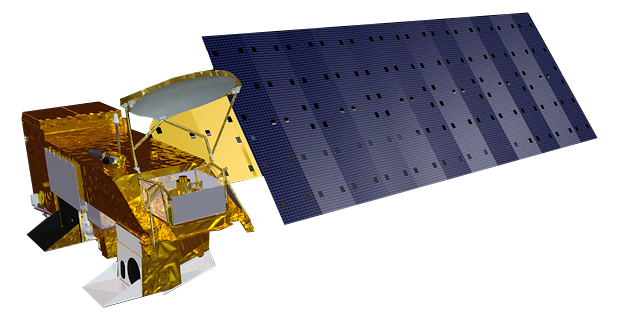
\includegraphics[width = 15cm]{Images/Aqua_spacecraft_model.png}
\end{figure}

\pagebreak

\section*{\Large REVISION HISTORY}

\begin{table}[h!]
\begin{center}
\begin{tabular} [0.9 \textwidth]{cl}
\hline \hline
\multicolumn{1}{c}{VERSION} & \multicolumn{1}{l}{REVISION NOTES} \\
\hline
PS1 & - Created document \\
    & - Added PS1 material \\
\hline
PS2 & - Cleaned up previous references and plots in PS1 material \\
    & - Added euler propagation plots and analysis \\
    & - Added orbit propagation plots and analysis \\
    & - formatted references and added necessary citations \\
\hline
PS3 & - Revised PS2 plots in order to better show numerical integration results\\
    & - Added PS3 material\\
\hline 
PS4 & - Revised PS3 orbital frame animation \\
    & - Added PS4 material\\
\hline
PS5 & - Added PS5 material \\
\hline
PS6 & - Revised PS5 grammar \\
    & - Continued editing disturbance torque models \\
    & - Added PS6 material \\
\hline
PS7 & - Added PS7 material \\
\hline \hline
\end{tabular}
	\caption{Summary of project revisions.}
\end{center}
\end{table}
 
\newpage
\section*{\Large TABLE OF CONTENTS}
\makeatletter
\@starttoc{toc}
\makeatother
\newpage
%%%%%%%%%%%%%%%%%%%%%%%%%%%%%%%%%%%%%%%%%%%%%%%%%%%%%%%%%%%%%%%%%%%%%%%%%%%%%%%%%%%%%%%%%%%%%%%%%%%%%%%%%%%%%%%%%%%%%%%%%%%%%%%%%%%%%%%%%%%%%%%%%%%%%%%%%%%%%%%%%%%%%%%%%%%%%%%%%%%%%%%%%%%%%%%%%%%%%%%%%%%%%%%%%%%%%%%%%%%

\section{\Large INTRODUCTION}

\section{\Large PROBLEM SET 1}
\subsection{PROBLEM 1}

\subsubsection{Select the characteristics of your mission.} \label{sec:char}

For this mission, we have decided to create an attitude determination and control system (ADCS) for a Low Earth Orbit (LEO) satellite that is Earth pointing. We are currently planning to use Euler Angles for our attitude state representation as we do not currently believe that the attitude adjustments needed for this mission will be large enough to lead to gimbal lock, the most typical problem that is faced when working with Euler angles. For the satellite's sensors, we are planning to use a magnetometer due to its reliability and a star tracker due to its high precision. The actuators that we are planning to use are reaction wheels and magnetorquers in order to have both large adjustment and fine tuning attitude maneuver capabilities.

\subsubsection{Conduct survey of satellites which have characteristics similar to selected project.}

Outside of communications satellites, Earth observing satellites are the most common type of satellites orbiting Earth today. Additionally, earth observing satellite missions generally have clear ADCS requirements due to the instrument payloads having resolution requirements that are publicly available. Due to these factors, analysis was done on several Earth observing satellites including the Landsat series of satellites \cite{landsat} and satellites carrying a MODIS (Moderate Resolution Imaging Spectrometer). \cite{mril} In this process, satellite missions that had released a sufficient amount of public information to make accurate conclusions about their ADCS systems, geometry, and mission requirements were favored over those that were withholding large amounts of information from the public.

\subsubsection{Select preferred existing satellite and payload for project.}

Out of the Earth observing satellites that were considered, the Aqua satellite from NASA seemed to closely match the characteristics that we had chosen in Section \ref{sec:char} and had a wealth of public information that we could use for the research and development of this mission.

\subsubsection{Collect basic information on mission, requirements, ADCS sensors and actuators, mechanical layout, mass, mass distribution, and inertia properties.} \label{sec:mission_info}

At the time of its launch in 2004, Aqua's primary mission objective was to collect data on the Earth's water cycle. This included observations related to oceans, atmosphere, land surfaces, and ice. Aqua eventually became a part of NASA's Earth Observing System (EOS) program, which aims to provide long-term data records for studying Earth's climate system and environmental changes over time. For its orbit, Aqua was in a Sun-Synchronous Orbit (SSO). The orbit was almost circular and had an altitude of 705 kilometers and an inclination of 98.2 degrees. \cite{aqua_orbit_info} The primary requirements of Aqua's mission were:

\begin{enumerate}
    \item Provide global coverage of Earth's surface to get the full picture of the Earth's water cycle and related phenomena. \\
    \item Obtain high spacial and temporal resolution to accurately capture changes in Earth's surface. \\
    \item Utilize multisensor and multispectral observations to ensure accurate data. \\
    \item Have a minimum mission lifetime of 6 years to ensure that changes in Earth's water cycle could be recorded over a lengthy amount of time. \\
    \item Have readily accessible data for analysis by the scientific community. 
\end{enumerate}

For its ADCS sensors, Aqua used two charged-couple-device (CCD) star trackers, an inertial reference unit package (IRU) that included a set of gyros, and a magnetometer. For its actuators, Aqua used four reaction wheels, a magnetic torquer assembly, and a set of four primary thrusters and four redundant backups. \cite{aqua_acds}

Like most satellites, the primary components of the Aqua satellite were the satellite structure that provided protection and support for all of the onboard instruments, the payload compartment that contained the suite of sensors for the mission, the power and thermal control subsystems, the ADCS, the communications subsystem, the on board computer (OBC), and the solar array. \cite{aqua_health_summary}

From combining some reference schematics and the known deployed dimensions of the satellite that were 4.81 meters (15.8 ft) x 16.70 meters (54.8 ft) x 8.04 meters (26.4 ft), a rough design of the outer mechanical layout was created and is shown in the following sections. \cite{aqua_mass_sumaries} Additionally, this schematic showing the sensor distribution that was obtained.

\begin{figure}[H]
    \centering
    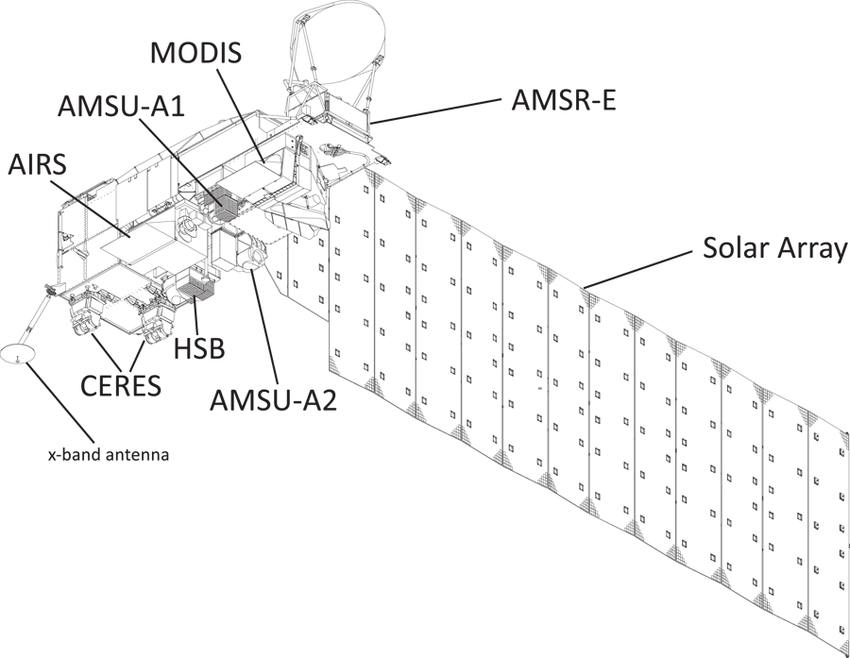
\includegraphics[width = 10cm]{Images/Schematic-of-the-Aqua-spacecraft-its-six-Earth-observing-instruments-12-panel-solar.png}
    \caption{Schematic of Aqua Instruments}
    \label{fig:squa-schematic}
\end{figure}

Additionally, the total mass of the satellite was 2,934 kg at launch. The mass distribution was 1,750 kg for the spacecraft structure, 1,082 kg for the instruments, and 102 kg for the propellant. Going into more detail, the individual mass of each of the instuments shown in Figure \ref{fig:squa-schematic} was also obtained. The MODIS had a mass of 229 kg. The AIRS had a mass of 177 kg. The AMSU-A had a mass of 91 kg. The HSB had a mass of 51 kg. The AMSR-E had a mass of 314 kg. Finally, the CERES had a mass of 50 kg per sensor of which there are two. It can be seen that with these instrument masses, their sum is 962 kg. Therefore, the mass of the overall system after both launch and deployment would have been 2814 kg. \cite{aqua_mass_sumaries} Even though the mass distribution and inertia properties of Aqua are not public information, by combining this information with Figure \ref{fig:squa-schematic}, a rough mass distribution and inertia properties such as the center of mass and moment of inertia can be obtained.

\subsubsection{Simplify spacecraft geometry, make assumptions on mass distribution, e.g. splitting it in its core parts, define body axes (typically related to geometry and payload), compute moments of inertia and full inertia tensor w.r.t. body axes. Show your calculations.}

A model of the satellite was generated with the geometry greatly simplified as shown in Figure \ref{fig:aquacad}. Each instrument listed in the previous section was approximated as a rectangular prism with a uniform mass distrubution corresopnding to the aforementioned instrument masses in Section \ref{sec:mission_info}. 


\begin{figure}[H]
    \centering
    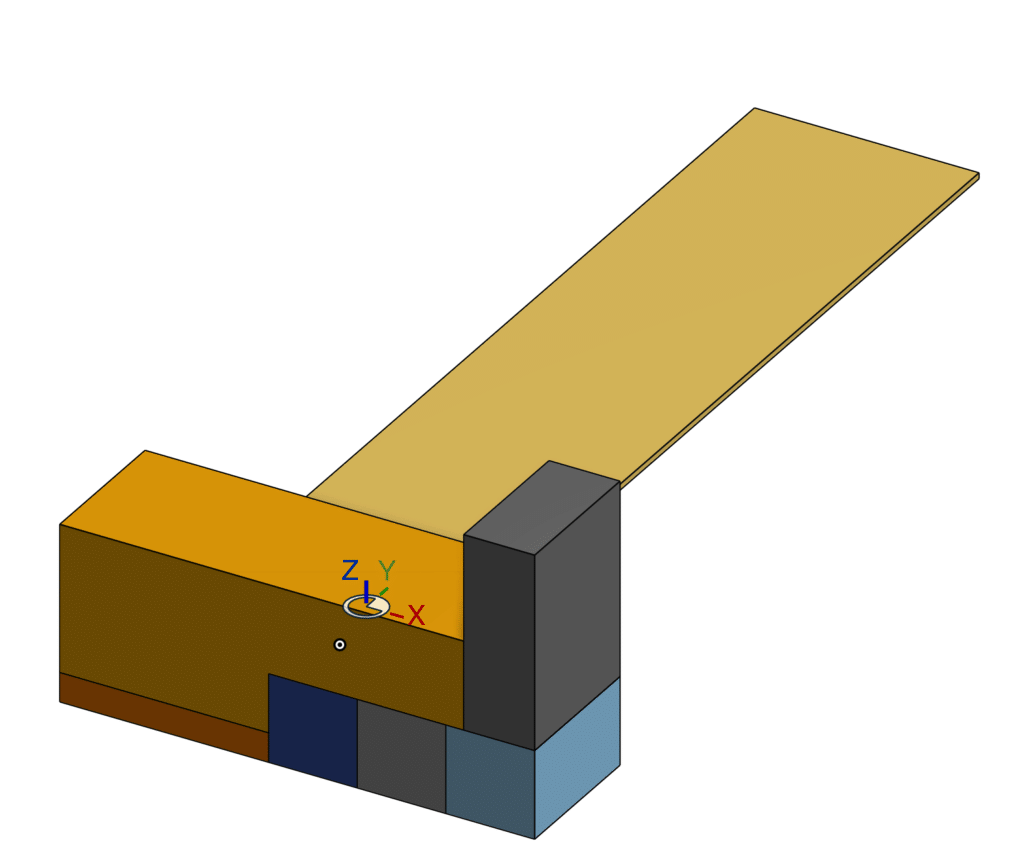
\includegraphics[width = 10cm]{Images/AquaSat-1.png}
    \caption{Simplified Aqua Model}
    \label{fig:aquacad}
\end{figure}

The location of the center of mass was calculated using Equation \ref{eq:center_mass} with distances measured from the lower-most corner oriented with the body coordinate system, whose orientation is  depicted in Figure \ref{fig:aquacad}. 

\begin{equation} \label{eq:center_mass}
    \vec{r} = \begin{bmatrix}
        \bar{x} & \bar{y} & \bar{z}
    \end{bmatrix}^T = \begin{bmatrix}
        \frac{\sum_{i=1}^N{m_i x_i}}{\sum_{i = 1}^N{m_i}} & \frac{\sum_{i=1}^N{m_i y_i}}{\sum_{i = 1}^N{m_i}} & \frac{\sum_{i=1}^N{m_i z_i}}{\sum_{i = 1}^N{m_i}}
    \end{bmatrix}^T
\end{equation}

The vector in this equation represents a position vector of the satellite's center of mass. The mass of each component in the satellite is denoted by $m_i$ where the position vector of each components center of mass has coordinates described as $\vec{r_i} = \begin{bmatrix}
    x_i & y_i & z_i
\end{bmatrix}^T$. The calculations were done using the component masses and locations tabulated below, which were pulled from the CAD model. The total mass along with the location of the satellite's center of mass is presented in the bottom row of Table \ref{tab:mass_props}. The mass of the chassis and solar panel were approximated by summing the non-instrument mass and propellant mass and uniformly distributing it between the two components.

\begin{table}[H]
    \centering
    \begin{tabular}{c|cccc}
    Component & $m_i$ [kg] & $x_i$ [m] & $y_i$ [m] & $z_i$ [m] \\ \hline
    MODIS     &    229   &    7.29   &   1.25    &   0.75    \\
    AMSU-A1   &     49  &    5.79   &    1.25   &   0.75    \\
    AMSU-A2    &    42   &    4.665   &   1.875    &  0.75   \\
    AIRS        &    177   &    4.29   &   0.625    &   0.75    \\
    HSB         &    51   &     3.915  &    1.875   &    0.75   \\
    CERES       &   100    &    1.77   &   1.25    &   0.25    \\
    AMSR-E      &    314   &    7.44   &    1.25   &   3.15    \\
    Chassis     &     1607  &    2.997   &   1.25    &    1.929   \\
    Solar Panel     &   245    &   4.02    &   9.6    &    2.25   \\ \hline
    Total       & 2184      & 4.059     & 1.958     & 1.804
    \end{tabular}
    \caption{Mass Properties and Distribution for Satellite Components}
    \label{tab:mass_props}
\end{table}

Following this, the moment of inertia for the satellite was computed. To compute this, first the moments of inertia of each component were taken about their own centers of mass. In general, the moment of inertia of a body is calculated using Equation \ref{eq:general_inertia}. Approximating each of the components as a rectangular prism, the moment of inertia about the centers of mass is found through using Equation \ref{eq:rect_inertia}, where $\rho$ is the mass density and $l_x$, $l_y$, and $l_z$ represent the lengths of each prism along the coordinate directions.

\begin{equation} \label{eq:general_inertia}
    \boldsymbol{I_{CM}} = \left[ \begin{array}{ccc}
     \int{(y^2 + z^2)}dm & \int{-  xy}dm & \int{-  xz}dm \\
\int{-  xy}dm &   \int{(x^2 + z^2)}dm & \int{-  yz}dm \\
\int{-  xz}dm & \int{-  yz}dm &  \int{(x^2 + y^2)}dm \\
    \end{array} \right]
\end{equation}

\begin{equation} \label{eq:rect_inertia}
    \boldsymbol{I_{CM}} = \left[ \begin{array}{ccc}
       \frac{1}{12}\rho l_x \left( l_y^3 l_z + l_z^3 l_y \right)  & 0 & 0 \\
         0  & \frac{1}{12}\rho l_y \left( l_x^3 l_z + l_z^3 l_x \right) & 0 \\
         0  & 0 &  \frac{1}{12}\rho l_z \left( l_x^3 l_y + l_y^3 l_x \right)
         \end{array} \right]
\end{equation}

Table \ref{tab:mass_props} shows the properties that were used to calculate the moment of inertias as well as the component-wise results. 

\begin{table}[H]
    \centering
    \begin{tabular}{c|ccccccc}
    Component & $\rho$ [kg/m\textsuperscript{3}] & $l_x$ [m] & $l_y$ [m] & $l_z$ [m] & $I_{xx}$ [kg m\textsuperscript{2}] & $I_{yy}$ [kg m\textsuperscript{2}] & $I_{zz}$ [kg m\textsuperscript{2}] \\ \hline
    MODIS       &    40.711    &   1.50    &   2.50     &  1.50     &  612.21      &  85.875      &   162.21     \\
    AMSU-A1     &    8.7111    &   1.50    &   2.50     &  1.50     &  34.708     &   18.375     &    34.708    \\
    AMSU-A2     &    29.867    &   0.75    &   1.25     &  1.50     &  13.344     &   9.814     &   7.438     \\
    AIRS        &    62.933    &   1.50    &   1.25     &  1.50     &  56.234     &   66.375     &  56.234      \\
    HSB         &    36.267    &   0.75    &   1.25     &  1.50     &  16.203     &   11.953     &  9.0310      \\
    CERES       &    22.599    &   3.54    &   2.50     &  0.50     &  54.167     &   106.51     &  156.51      \\
    AMSR-E      &    31.717    &   1.20    &   2.50     &  3.30     &  448.50     &   322.64     &  201.222      \\
    Solar Panel &    45.404    &   3.80    &   14.2    &   0.1    &    4117.0    &    295.00    &   4411.6     \\
    \end{tabular}
    \caption{Mass Properties and Distribution for Satellite Components}
    \label{tab:mass_props}
\end{table}

The chassis inertia had to be computed in a different manner using a composition of rectangles. The approach taken in this paper was to first take the inertia about a geometrically convenient point, then use the parallel axis theorem to determine the inertia about the center of mass of the chassis. The composition chosen was one where a larger rectangle of uniform density has from it a component of equivalent density subtracted. This composition is described in Table \ref{tab:composite_chassis}.

\begin{table}[H]
    \centering
    \begin{tabular}{c|ccccccc}
    Member  & $\rho$ & $l_x$ & $l_y$ & $l_z$ & $I_{xx}$ & $I_{yy}$ & $I_{zz}$ \\ \hline
    Prism 1 &   46.580     &   6.84    &   2.5    &   2.5    &  2074.3      &   8800.7     &   8800.7     \\
    Prism 2 &   -46.580     &  3.3     &   2.5    &   1.0    &  232.17      &   380.76     &   548.88     \\  
    \end{tabular}
    \caption{Mass Properties for Composite Chassis}
    \label{tab:composite_chassis}
\end{table}

Using the parallel axis theorem, seen in Equation \ref{eq:par_axis}, the moment of inertia of the composite shape about the center of mass of prism 1 along with the inertia about the center of mass of the object is shown in Table \ref{tab:chass_inertia}. In Equation \ref{eq:par_axis}, $\boldsymbol{I_P}$ is the inertia tensor about an arbitrary point P whose position relative to the center of mass is $\vec{r} = \begin{bmatrix} x & y & z \end{bmatrix}^T$.

\begin{equation} \label{eq:par_axis}
    \boldsymbol{I_{P}} = \boldsymbol{I_{CM}} + m \left[ \begin{array}{ccc}  (y^2 + z^2) & -  xy & -  xz \\ 
    -  xy &   (x^2 + z^2) & -  yz \\
-  xz & -  yz &  (x^2 + y^2) \\ \end{array} \right]
\end{equation}


\begin{table}[H]
    \centering
    \begin{tabular}{c|cccccc}
    Reference Point   & $I_{xx}$ & $I_{yy}$ & $I_{zz}$ & $I_{xy}$ & $I_{xz}$ & $I_{yz}$ \\ \hline
    Center of Prism 1 & 1625.9   & 7000     & 7047.9   & 0        & -510.10  & 0        \\
    Center of Mass    & 1574.2   & 6660.3   & 6760.0   & 0        & -632.12  & 0       
    \end{tabular}
    \caption{Inertia Tensors of Chassis about Intermediate Reference and Center of Mass}
    \label{tab:chass_inertia}
\end{table}

Now applying parallel axis theorem to each component, Aqua's inertia tensor about its own center of mass is shown in Table \ref{tab:total_ineretia}.

\begin{table}[H]
\centering
\begin{tabular}{c|cccccc}
                     & $I_{xx}$ & $I_{yy}$ & $I_{zz}$ & $I_{xy}$ & $I_{xz}$ & $I_{yz}$ \\ \hline
Total Inertia Tensor & 23745    & 17560    & 36065    & 93.907   & -1267.1  & -967.50 
\end{tabular}
\caption{Total Inertial Tensor about Satellite Center of Mass Directed along Body Axes}
\label{tab:total_ineretia}
\end{table}

Below is the script written to perform all of the above calculations.

\begin{lstlisting}
clc, clear 
close all

%% Instrument Moments of Inertia

instruments = {'MODIS', 'AMSU-A1', 'AMSU-A2', 'AIRS', 'HSB', 'CERES', 'AMSR-E'};
lxs = [1.5, 1.5, 0.75, 1.5, 0.75, 3.54, 1.2];
lys = [2.5, 2.5, 1.25, 1.25,1.25, 2.5, 2.5];
lzs = [1.5, 1.5, 1.5, 1.5, 1.5, 0.5, 3.3];
ms = [229, 49, 42, 177, 51, 100, 314];
Vs = lxs.*lys.*lzs;
rhos = ms./Vs;
Icms = zeros([3 3 7]);

for i = 1:7
    Icms(:,:,i) = rectInertia(lxs(i),lys(i),lzs(i),rhos(i));
end
%% Chassis

V = 34.5;
Vsub = 3.3*2.5*1;
Vt = V + Vsub;
m = 1607;
rho = m/V;

It = rectInertia(6.84, 2.5, 2.5, rho);

Is = rectInertia(3.3,2.5,1,rho);

xbar = 1.77;
ybar = 0;
zbar = -0.75;

Is = parallelAxis(Is,xbar,ybar,zbar,rho,Vsub);

Ichassis = It - Is;

xbart = 3.42;
ybart = 1.25;
zbart = 1.75;

xbars = xbart + xbar;
ybars = ybart + ybar;
zbars = zbart + zbar;

xbarc = (Vt*xbart - Vsub*xbars)/V
ybarc = (Vt*ybart - Vsub*ybars)/V
zbarc = (Vt*zbart - Vsub*zbars)/V

xtild = xbart - xbarc;
ytild = ybart - ybarc;
ztild = zbart - zbarc;

Ichassis = parallelAxis(Ichassis, xtild, ytild, ztild, -rho, V)

%% Solar Panel

lx = 3.8;
ly = 14.2;
lz = 0.1;
V = lx*ly*lz;
m = 245;
rho = m/V;

Isolar = rectInertia(lx,ly,lz,rho);

%% COM

ms = [ms, 1607, 245];
Vs = [Vs, 34.5, 5.396];
rhos = ms./Vs;
Icms = cat(3, Icms, Ichassis, Isolar);

xis = [7.29, 5.79, 4.665, 4.29, 3.915, 1.77, 7.44, xbarc, 8.04/2];
yis = [1.25, 1.25, 1.875, 0.625, 1.875, 1.25, 1.25, ybarc, 9.6];
zis = [0.75, 0.75, 0.75, 0.75, 0.75, 0.25, 3.15, zbarc, 2.25];

xyzBar = centerMass(ms, xis, yis, zis);

%% Total Moment of Inertia

% xis(8) = 6.84/2;
% zis(8) = 1.75;

x0s = xis - xyzBar(1);
y0s = yis - xyzBar(2);
z0s = zis - xyzBar(3);

Itotal = zeros([3 3]);

for i=1:9
    Itotal = Itotal + parallelAxis(Icms(:,:,i), x0s(i), y0s(i), z0s(i), rhos(i), Vs(i));
end

%% Functions

function I = rectInertia(lx, ly, lz, rho)

% rho = m/V;

I = zeros([3 3]);

% Ixy = 0, Iyz = 0, Ixz = 0;

Ixx = (1/12).*rho.*lx.*(ly.^3.*lz + lz.^3.*ly);
Iyy = (1/12).*rho.*ly.*(lx.^3.*lz + lz.^3.*lx);
Izz = (1/12).*rho.*lz.*(lx.^3.*ly + ly.^3.*lx);

I(1,1) = Ixx;
I(2,2) = Iyy;
I(3,3) = Izz;

end

function I = parallelAxis(Icm, x, y, z, rho, V)

Iplus = rho*V*[y^2 + z^2, -x*y, -x*z;
            -x*y, x^2 + z^2, -y*z;
            -x*z, -y*z, x^2 + y^2];

I = Icm + Iplus;

end

function xyzBar = centerMass(ms, xs, ys, zs)

xbar = sum(xs.*ms)/sum(ms);
ybar = sum(ys.*ms)/sum(ms);
zbar = sum(zs.*ms)/sum(ms);

xyzBar = [xbar, ybar, zbar];

end
\end{lstlisting}

\subsubsection{Discretize your spacecraft through its outer surfaces (geometry). Develop a Matlab/Simulink function to handle barycenter (geometry, no mass distribution) coordinates, size, and unit vectors normal to each outer surface of the spacecraft in body frame. You can list all this information in a Matrix. }

Descriptions of all surfaces through barycenter coordinates, surfaces normal vectors, and surface areas are recorded below in Table \ref{tab:surface_data} with the corresponding surfaces labeled in Figure \ref{fig:surface_labels}. 

% Please add the following required packages to your document preamble:
% \usepackage{multirow}
\begin{table}[H]
\centering
\begin{tabular}{c|ccc|ccc|c}
        & \multicolumn{3}{c|}{Surface Normal Vector} & \multicolumn{3}{c|}{Centroid Coordinates} & \multirow{2}{*}{Area [m\textsuperscript{2}]} \\ \cline{2-7}
Surface & $n_x$        & $n_y$        & $n_z$        & $x$ [m]  & $y$ [m]  & $z$ [m] &                                                                   \\ \hline
1       & 0            & -1           & 0            & 4.30         & 0            & 1.70        & 26.28                                                             \\
2       & 1            & 0            & 0            & 8.04         & 1.25         & 2.40        & 12.00                                                             \\
3       & 0            & 0            & 1            & 7.44         & 1.25         & 4.80        & 3.000                                                             \\
4       & -1           & 0            & 0            & 0            & 1.25         & 1.5         & 7.500                                                             \\
5       & 0            & 0            & 1            & 3.42         & 1.25         & 3.00        & 17.10                                                             \\
6       & 0            & 0            & 1            & 4.02         & 9.60         & 2.30        & 53.96                                                             \\
7       & 0            & 0            & -1           & 4.02         & 9.60         & 2.30        & 53.96                                                             \\
8       & -1           & 0            & 0            & 6.84         & 1.25         & 3.90        & 4.500                                                             \\
9       & 0            & 1            & 0            & 4.30         & 0            & 1.70        & 26.28                                                             \\
10      & 0            & 0            & -1           & 4.02         & 1.25         & 0           & 20.10                                                            
\end{tabular}
\caption{Normal Vectors, Barycenter Coordinates, and Surface Area for All Outer Surfaces}
\label{tab:surface_data}
\end{table}

\begin{figure}[H]
    \centering
    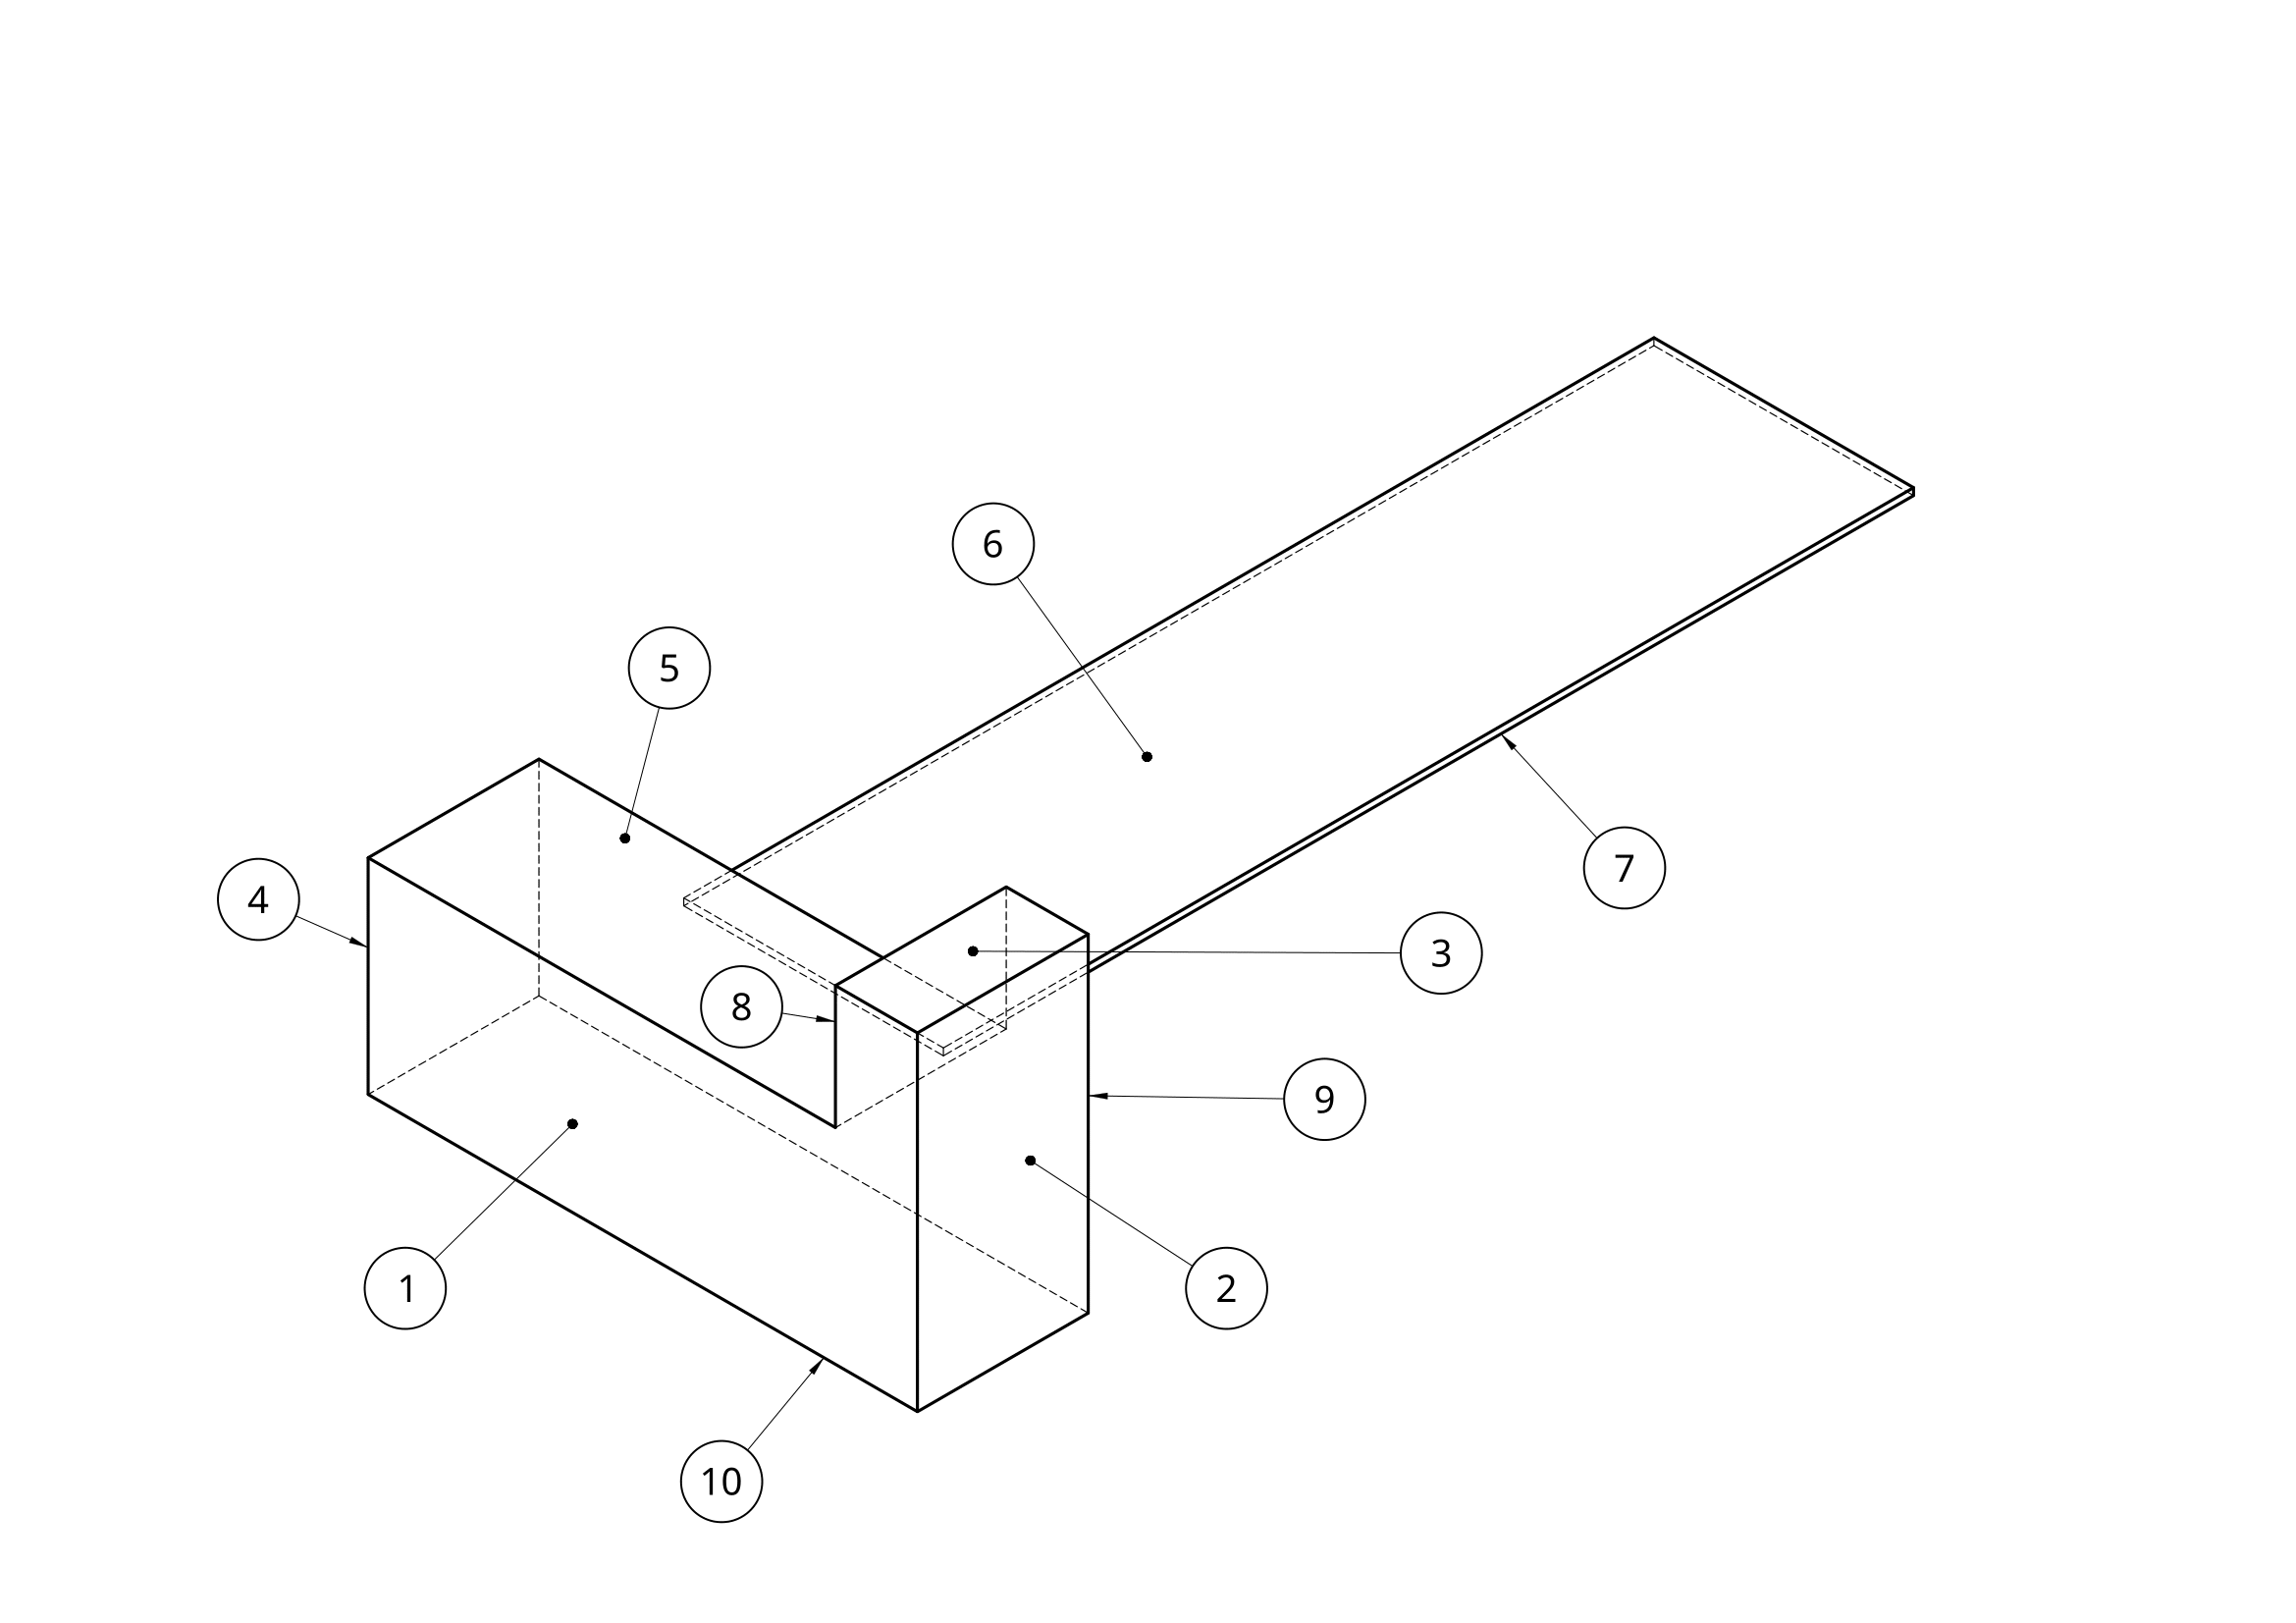
\includegraphics[width = 14cm]{Images/AquaSurfaces.png}
    \caption{Schematic of Aqua's Outer Surfaces Discretized and Labeled}
    \label{fig:surface_labels}
\end{figure}

The script that was used to store this data is seen below:


\begin{lstlisting}
clc, clear
close all

A1s = [6.84*3, 1.2*4.8].';
P1s = [6.84/2, 0, 3/2;
        6.84 + 1.2/2, 0, 4.8/2];
[A1, P1] = cent(A1s, P1s);
A9 = A1; P9 = P1;
N1 = [0 -1 0]; N9 = -N1;

A2 = 4.8*2.5;
P2 = [8.04, 2.5/2, 4.8/2];
N2 = [1 0 0];

A3 = 1.2*2.5;
P3 = [6.84 + 1.2/2, 2.5/2, 4.8];
N3 = [0 0 1];

A4 = 2.5*3;
P4 = [0 2.5/2, 3/2];
N4 = [-1 0 0];

A5 = 2.5*6.84;
P5 = [6.84/2, 2.5/2, 3];
N5 = [0 0 1];

A6 = 14.2*3.8; A7 = A6;
P6 = [4.02, 9.6, 2.3]; P7 = P6;
N6 = [0 0 1]; N7 = -N6;

A8 = 2.5*1.8;
P8 = [6.84, 2.5/2, 3 + 1.8/2];
N8 = [-1 0 0];

A10 = 8.04*2.5;
P10 = [8.04/2, 2.5/2, 0];
N10 = [0 0 -1];

N = [N1;N2;N3;N4;N5;N6;N7;N8;N9;N10];
A = [A1;A2;A3;A4;A5;A6;A7;A8;A9;A10];
P = [P1;P2;P3;P4;P5;P6;P7;P8;P9;P10];

%% Centroid Function
function [Ai, Pi] = cent(As, Ps)

Ai = sum(As);

x = sum(Ps(:,1).*As)./Ai;
y = sum(Ps(:,2).*As)./Ai;
z = sum(Ps(:,3).*As)./Ai;

Pi = [x, y, z];

end
\end{lstlisting}
\section{\Large PROBLEM SET 2}
\subsection{Problem 2}

\subsubsection{Define orbit initial conditions and make sure you can propagate the orbit of the satellite over multiple orbits using either a Keplerian propagator or a numerical integration scheme.}

The orbit initial conditions were chosen to closely replicate those of the Aqua satellite. The orbit is sun-synchronous, has an eccentricity of almost zero, and has an altitude similar to that of Aqua.

\begin{center}
    a = 7080.6 km \\
    e = 0.0000979 \\
    i = 98.2\degree \\
    $\omega$ = 120.4799\degree \\
    $\Omega$ = 95.2063\degree \\
    $\nu$ = 0\degree
\end{center}

To propagate the orbit, these orbital elements were first converted to the initial position and velocity in the Earth centered Inertial (ECI) frame. The ECI frame is defined such that it doesn't rotate with Earth's surface. The x-axis points in the direction of the vernal equinox (the ascending node of the sun), the z-axis points towards the north pole, and the y-axis completes the triad. To initially propagate the orbit and serve as a point of reference, Simulink was used to sweep the mean anomaly over a given time span and time steps and calculate the position in the ECI frame at each time step. The Simulink model is shown below in Figure \ref{fig:simulink-prop}.

\begin{figure}[H]
    \centering
    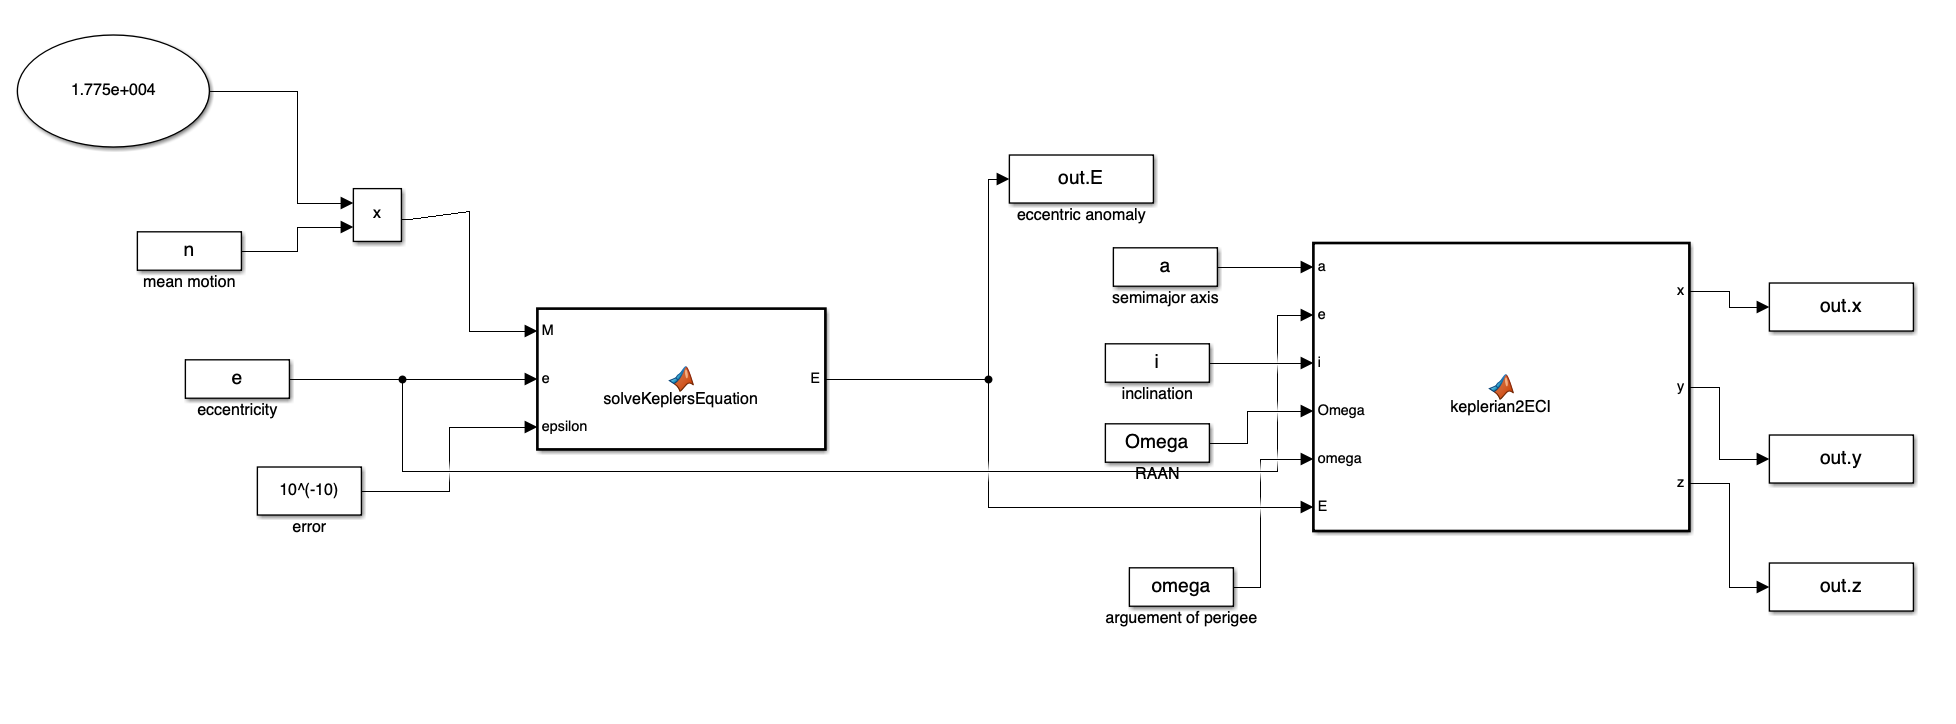
\includegraphics[width = 15.5cm]{Images/simulink_prop.png}
    \caption{Simulink Model for Keplerian Propagator}
    \label{fig:simulink-prop}
\end{figure}

The Keplerian propagator was then used to plot the orbit for a time span roughly equal to three orbital periods. The resulting orbit along with a spherical model of Earth is shown below in Figure \ref{fig:kep_orbit}.

\begin{figure}[H]
    \centering
    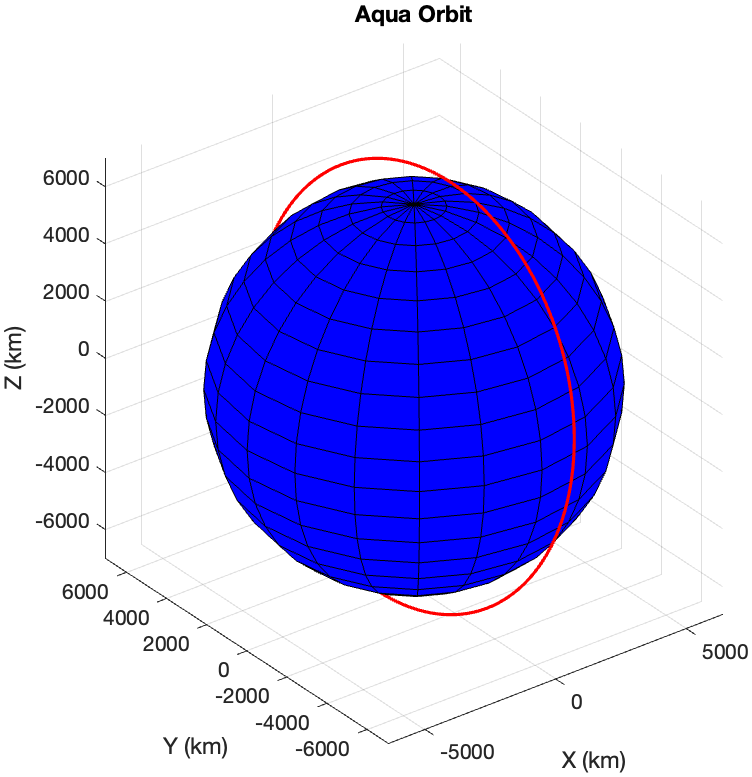
\includegraphics[width = 8.5cm]{Images/aqua_orbit_kepler.png}
    \caption{Aqua Orbit for Keplerian Propagator}
    \label{fig:kep_orbit}
\end{figure}

The Matlab function that was used for the Keplerian propagator can also be seen here.

\lstinputlisting{code}


\subsubsection{In general the body axes are not the principal axes. Identify principal axes through the eigenvector/eigenvalue problem discussed in class and compute the rotation matrix from body to principal axes.} \label{sec:principal_inertia_def_and_calc}

To resolve an inertia tensor $\boldsymbol{I_{CM}}$ to a diagonal matrix of principal moments of inertia, there must exist a matrix, $\boldsymbol{A}$ such that the Equation \ref{eq:principal_moments} holds, where $\boldsymbol{I_{CM}'}$ is the principal moment of inertia tensor about the center of mass.

\begin{equation} \label{eq:principal_moments}
    \boldsymbol{I_{cm} A} = \boldsymbol{A I_{CM}'} 
\end{equation}

It can be seen that the principal moments of inertia are the eigenvalues of the inertia tensor and that the matrix $\boldsymbol{A}$ is a matrix whose columns are the right eigenvectors or the inertia tensor. For the AQUA spacecraft, the results that follow are shown below.

\begin{equation*}
    \boldsymbol{I_{CM}'} = \begin{bmatrix}
        17510 & 0 & 0 \\
        0 & 23616 & 0 \\
        0 & 0 & 36245
    \end{bmatrix} \text{kg} \cdot \text{m}^2
\end{equation*}

\begin{equation*}
    \boldsymbol{A} = \begin{bmatrix}
            0.0045  &  0.9949 &  -0.1011 \\
            -0.9986  & -0.0007  & -0.0520 \\
            -0.0518  &  0.1012  &  0.9935
    \end{bmatrix}
\end{equation*}

\subsubsection{At this stage you should have a simple 3D model of your spacecraft including geometry and mass properties of each element. This includes at least two coordinate systems, body and principal axes respectively, and the direction cosine matrix between them. Plot axes of triads in 3D superimposed to spacecraft 3D mode}

The body axes of the spacecraft are seen plotted in Figure \ref{fig:aquacad}. The principal inertia axes are seen plotted in Figure \ref{fig:aquacad_principal}.

\begin{figure}[H]
    \centering
    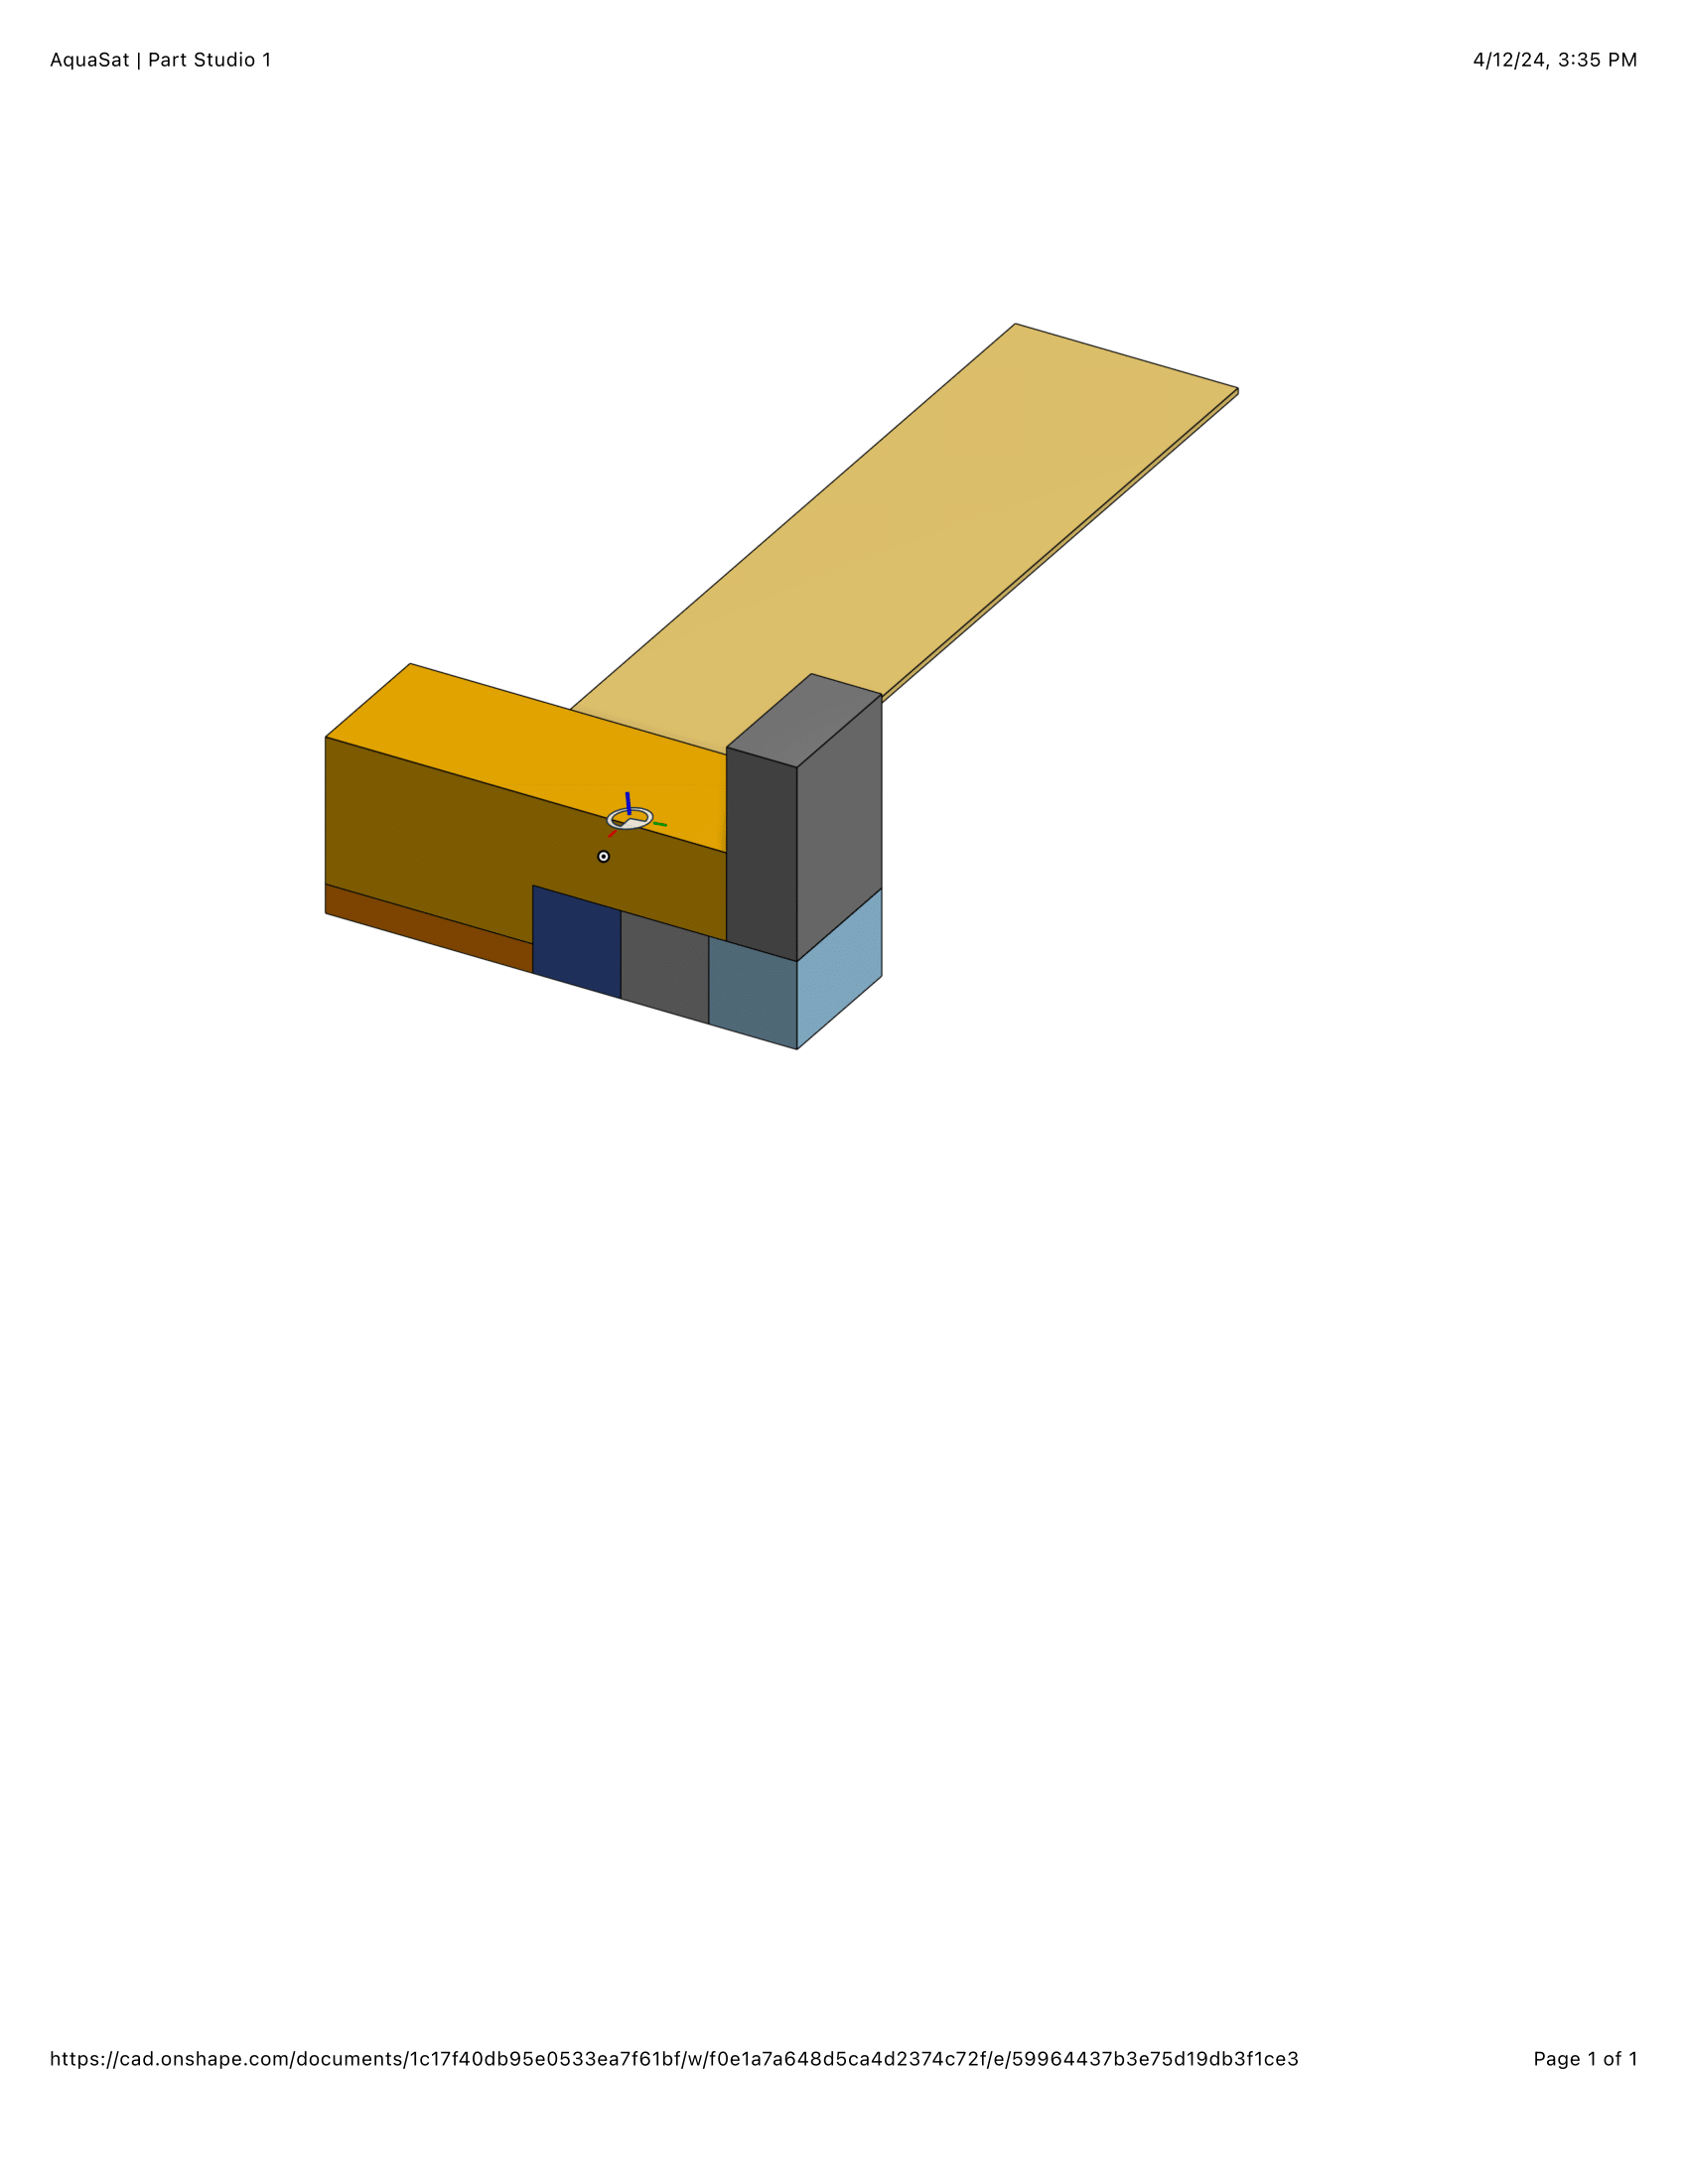
\includegraphics[width = 10cm]{Images/AquaSat_PrincipalAxes.png}
    \caption{Simplified Aqua Model with Principal Axes}
    \label{fig:aquacad_principal}
\end{figure}

\subsubsection{Program Euler equations in principal axes (e.g. in Matlab/Simulink). No external torques.}

The following Simulink model utilizing a MATLAB function (both in Figure \ref{fig:euler_prop_model}) takes in an initial rotational velocity vector and simulates the physics of the current AQUA model about the principal axes of inertia.

\begin{figure}[H]
    \centering
    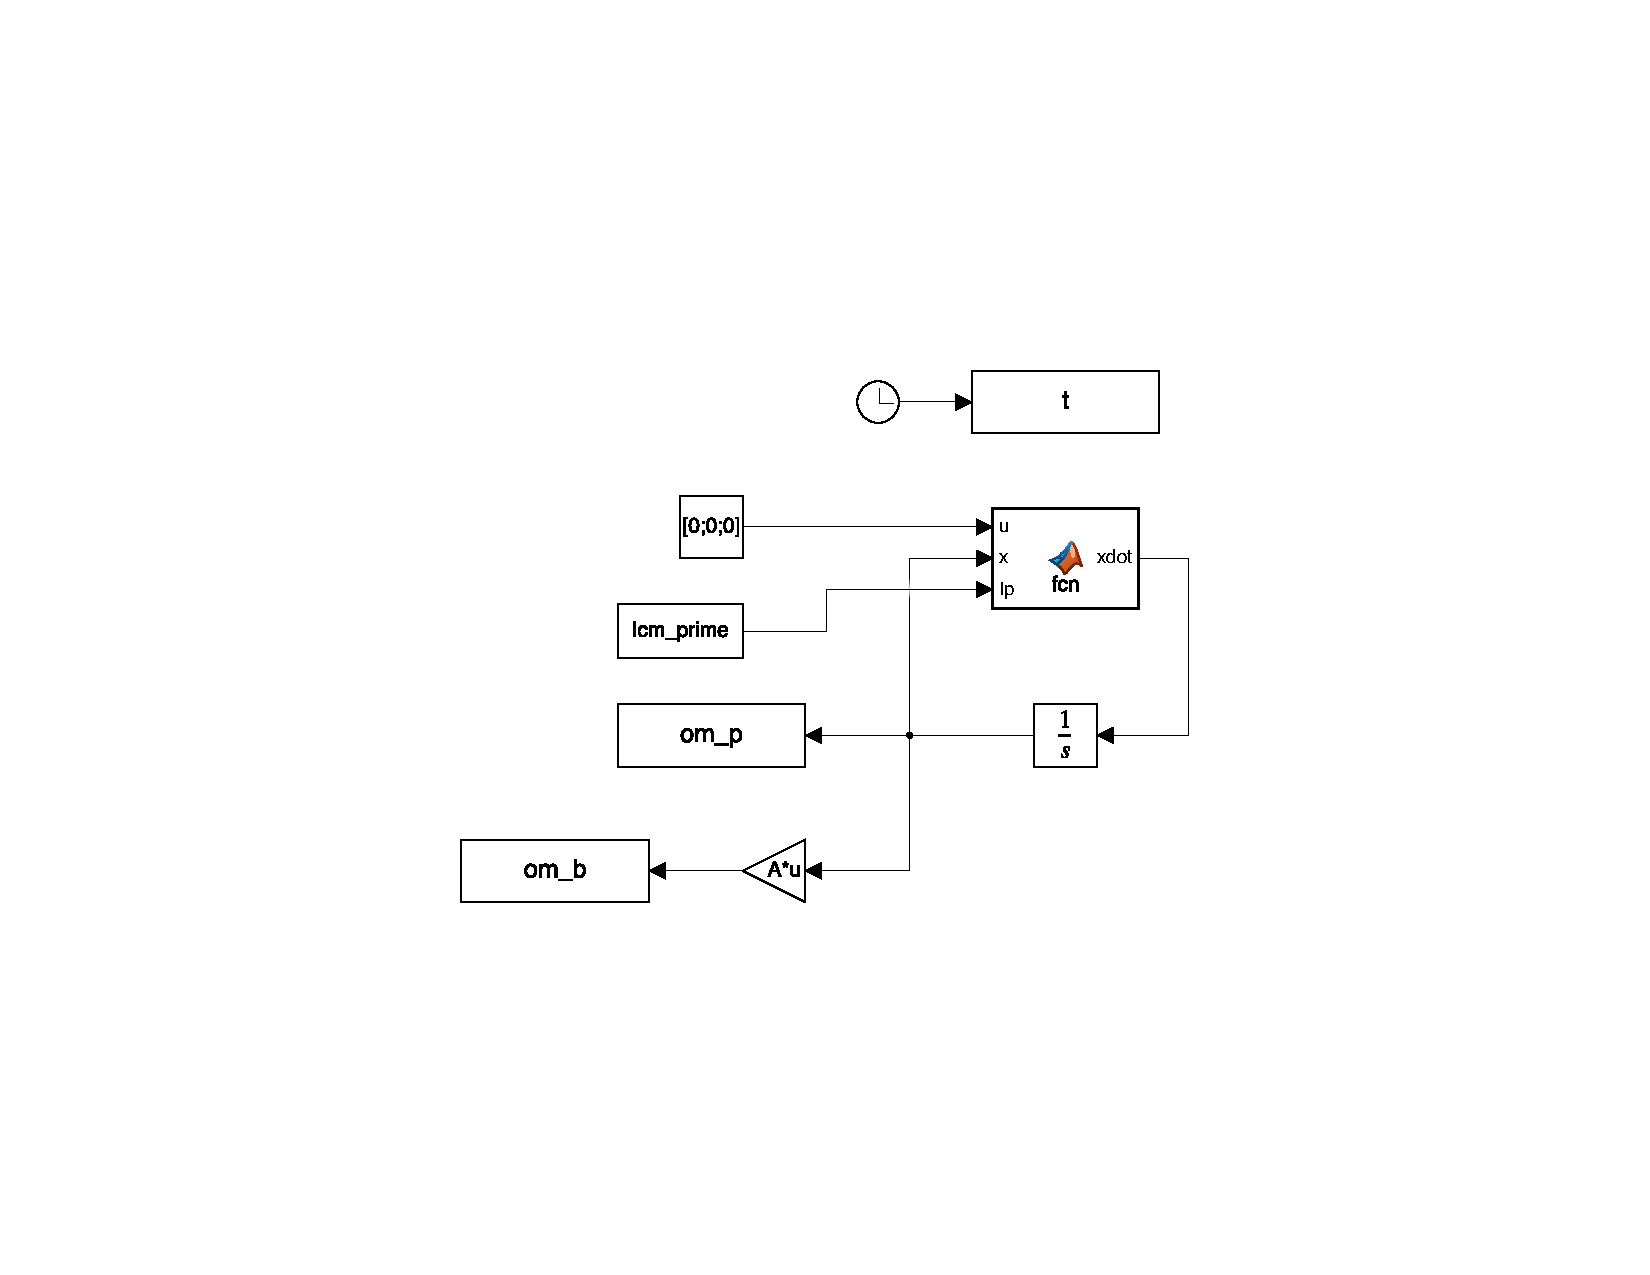
\includegraphics[trim={5cm 5cm 5cm 5cm},clip,width = 15cm]{Images/eulerPropagate.pdf}
\end{figure}

\begin{figure} [H]
    \centering
    \begin{lstlisting}
function xdot = fcn(u,x,Ip)

xdot = zeros(size(x));


Mx = u(1);
My = u(2);
Mz = u(3);

omx = x(1);
omy = x(2);
omz = x(3);

Ix = Ip(1,1);
Iy = Ip(2,2);
Iz = Ip(3,3);

wxdot = (1/Ix)*(Mx - (Iz - Iy)*omy*omz);
wydot = (1/Iy)*(My - (Ix - Iz)*omz*omx);
wzdot = (1/Iz)*(Mz - (Iy - Ix)*omx*omy);

xdot(1) = wxdot;
xdot(2) = wydot;
xdot(3) = wzdot;

end
    \end{lstlisting}
    \caption{Euler Propagation Simulink Model}
    \label{fig:euler_prop_model}
\end{figure}


\subsubsection{Numerically integrate Euler equations from arbitrary initial conditions ($\boldsymbol{\omega < 10^{\circ}/s}$, $\boldsymbol{\omega_i \neq 0}$). Multiple attitude revolutions.}

Given an initial condition of $\vec{\omega}_0 = \begin{bmatrix}
    -7 & 2 & 5
\end{bmatrix}^T {}^{\circ}/s$, gyroscopic coupling causes a periodic oscillation in the angular velocity vector represented in a body fixed axis frame. In this instance in particular, the simulation results shown in \ref{fig:sim_omegas} follows this evolution in the principal frame.

\begin{figure}[H]
    \centering
    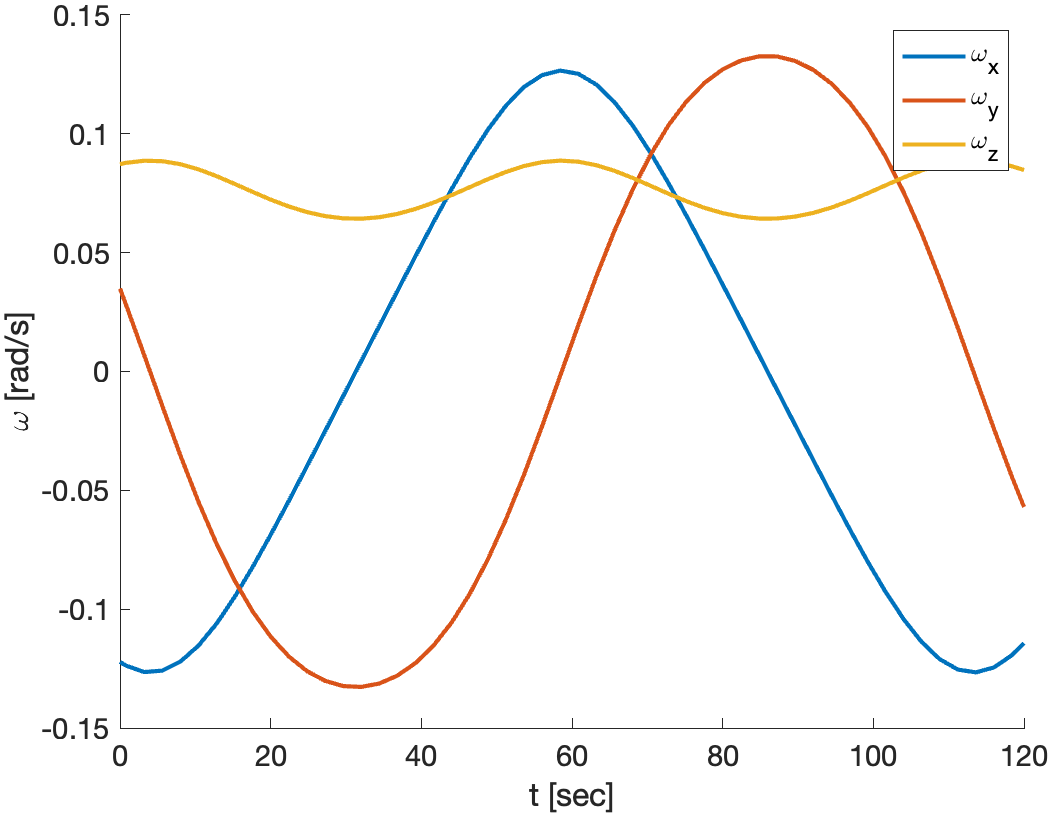
\includegraphics[width = 10cm] {Images/omega_prop_random.png}
    \caption{Angular Velocity Vector Components Evolving in the Body Fixed Principally Oriented Frame}
    \label{fig:sim_omegas}
\end{figure}

\subsubsection{Plot rotational kinetic energy and momentum ellipsoids in 3D (axis equal) corresponding to chosen initial conditions. Verify that semi-axis of ellipsoids corresponds to theoretical values} \label{sec:ellipsoid_definitions}

The angular momentum and rotational kinetic energy of a rigid body is computed using Equations \ref{eq:ang_mom} and \ref{eq:rot_KE} respectively, where $\vec{L}$ and $T$ are the momentum vector and energy, and the angular velocity vector in the principally oriented frame is described as $\vec{\omega} = \begin{bmatrix} \omega_x & \omega_y & \omega_z \end{bmatrix}^T$. 

\begin{equation} \label{eq:ang_mom}
    \vec{L} = \boldsymbol{I_{CM}'}\vec{\omega} = I_x \omega_x + I_y \omega_y + I_z \omega_z
\end{equation}

\begin{equation} \label{eq:rot_KE}
    T = \vec{\omega} \cdot \vec{L} = I_x \omega_x^2 + I_y \omega_y + I_z \omega_z^2
\end{equation}

These quantities are both conserved, so the satellite's angular velocity must always take on a vector value that yields the same momentum magnitude and kinetic energy as the initial conditions. With the initial conditions given above, the magnitude of angular momentum is 3906.4 kg m/s and the kinetic energy is 283.08 J. With not much manipulation, these relations can be shown to be equivalent to Equations \ref{eq:mom_ellipse} and \ref{eq:energy_ellipse} respectively, where L is the magnitude of the angular momentum vector.  

\begin{equation} \label{eq:mom_ellipse}
    \frac{\omega_x^2}{(L/I_x)^2} + \frac{\omega_y^2}{(L/I_y)^2} + \frac{\omega_z^2}{(L/I_z)^2} = 1
\end{equation}

\begin{equation} \label{eq:energy_ellipse}
    \frac{\omega_x^2}{2T/I_x} + \frac{\omega_y^2}{2T/I_y} + \frac{\omega_z^2}{2T/I_z} = 1
\end{equation}

By inspection, the form of these equations is that of an ellipsoid. Therefore, if the Cartesian coordinates are chosen such that the x,y, and z components of the angular velocity lie along the x,y, and z axes, the tip of the angular velocity vector plotted on these axes will lie on the surface of these ellipsoids. The momentum ellipsoid is plotted along with its semi-axis lengths is plotted in Figure \ref{fig:momentum_axis_verification}. The same is done for the energy ellipsoid in Figure \ref{fig:energy_axis_verification}

\begin{figure}[H]
    \centering
    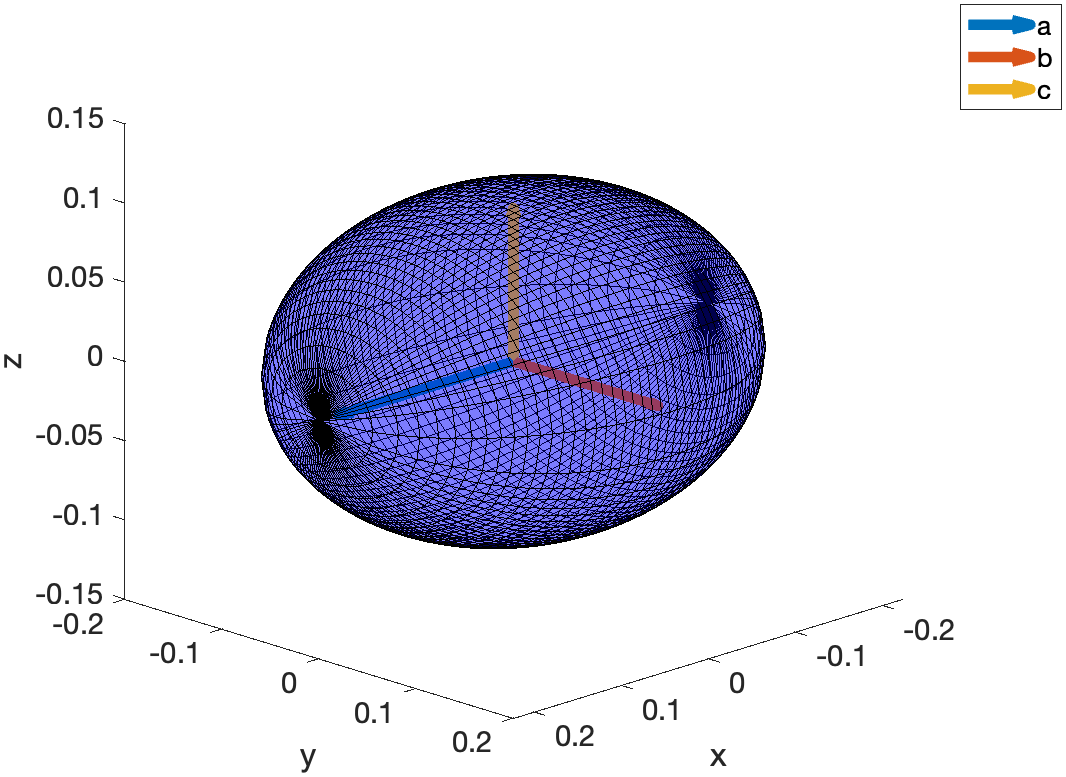
\includegraphics[width = 10cm]{Images/momentum_axes_random.png}
    \caption{Momentum Ellipsoid and Semi-Axis Lengths}
    \label{fig:momentum_axis_verification}
\end{figure}

\begin{figure}[H]
    \centering
    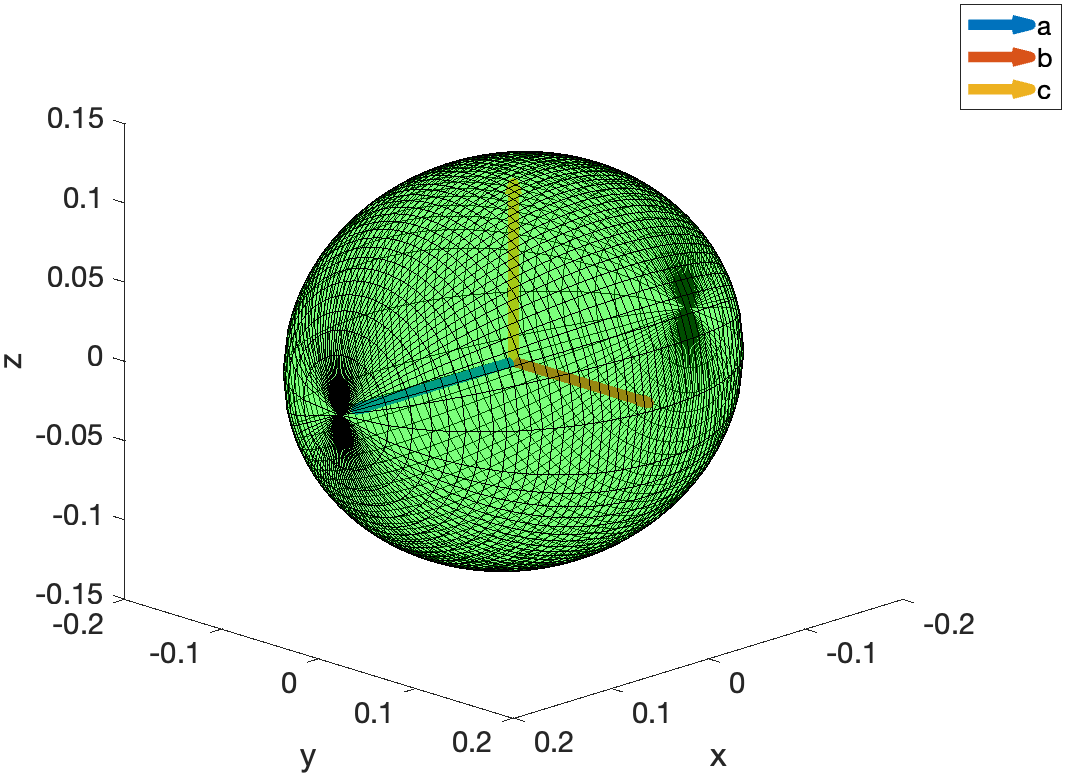
\includegraphics[width = 10cm]{Images/energy_axes_random.png}
    \caption{Energy Ellipsoid and Semi-Axis Lengths}
    \label{fig:energy_axis_verification}
\end{figure}

\subsubsection{Plot polhode in same 3D plot. Verify that it is the intersection between the ellipsoid}

Following that the angular velocity in a Cartesian plot must lie along the surface of both ellipsoids described in Section \ref{sec:ellipsoid_definitions}, it follows that the vector would be restricted to the intersection of the two ellipsoids. The curve that this vector traces is called the polhode, and the simulated results of this curve can be seen in Figure \ref{fig:ellipsoid_super_plot}, over-plotted with the momentum and energy ellipsoids. This curve matches the expected behavior in that it clearly traces the intersection between the momentum and energy ellipsoids. 

\begin{figure}[H]
    \centering
    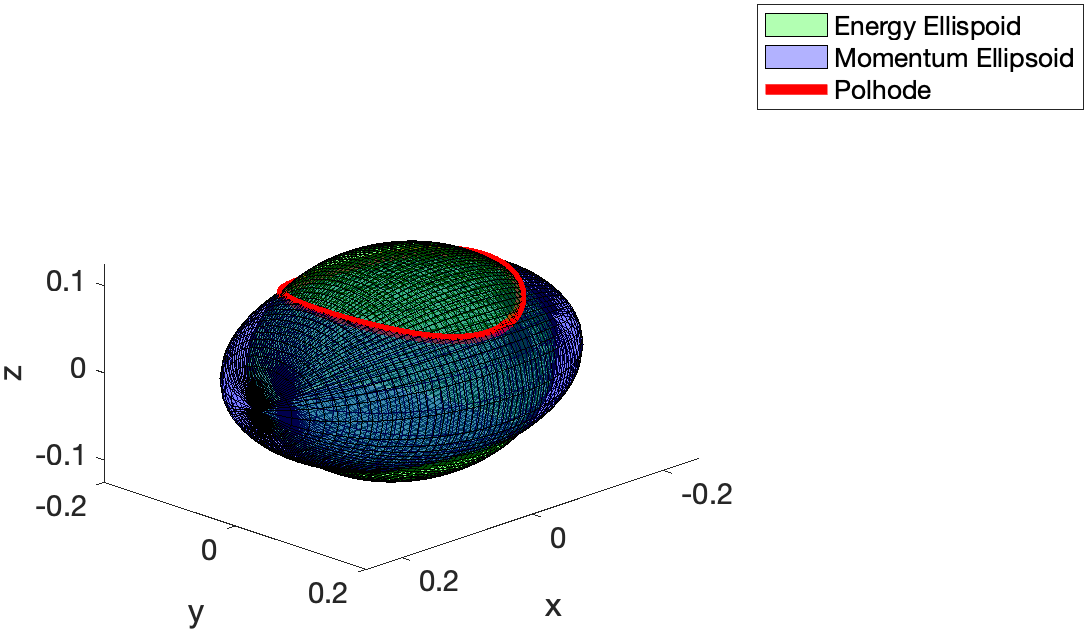
\includegraphics[width = 12cm] {Images/ellipsoid_polhode_random.png}
    \caption{Momentum and Energy Ellipsoids and Polhode Curve Plotted in 3D on Principally Aligned Coordinate Axes}
    \label{fig:ellipsoid_super_plot}
\end{figure}

\subsubsection{Plot polhode in three 2D planes identified by principal axes (axis equal). Verify that shapes of resulting conic sections correspond to theory.}

Figure \ref{fig:2d_polhode} shows the planar projections of the polhode curve along the labeled axes. In theory, these curves should be described by Equations \ref{eq:polhode1}, \ref{eq:polhode2}, and \ref{eq:polhode3}. 

\begin{equation} \label{eq:polhode1}
    (I_y - I_x)I_y \omega_y^2 + (I_z - I_x)I_z \omega_z^2 = L^2 - 2TI_x
\end{equation}

\begin{equation} \label{eq:polhode2}
    (I_x - I_y)I_x \omega_x^2 + (I_z - I_y)I_z \omega_z^2 = L^2 - 2TI_y
\end{equation}

\begin{equation} \label{eq:polhode3}
    (I_x - I_z)I_x \omega_x^2 + (I_y - I_z)I_y \omega_y^2 = L^2 - 2TI_z
\end{equation}

Due to the fact that $I_x < I_y < I_z$, Equation \ref{eq:polhode1} describes an ellipse in the yz plane, Equation \ref{eq:polhode2} a hyperbola in the xz plane, and Equation \ref{eq:polhode3} another ellipse in the xy plane. The theoretical values obtained from these equations were plotted over the polhode that resulted from simulations in Figure \ref{fig:2d_polhode}, establishing that the simulated dynamics followed the expected behavior. Additionally, these equations imply that $I_x < L^2/2T < I_y$. With these initial conditions, this quantity evaluates to 26954 kg m\textsuperscript{2} which lies within the specified bounds described in \ref{sec:principal_inertia_def_and_calc}.

\begin{figure}[H]
    \centering
    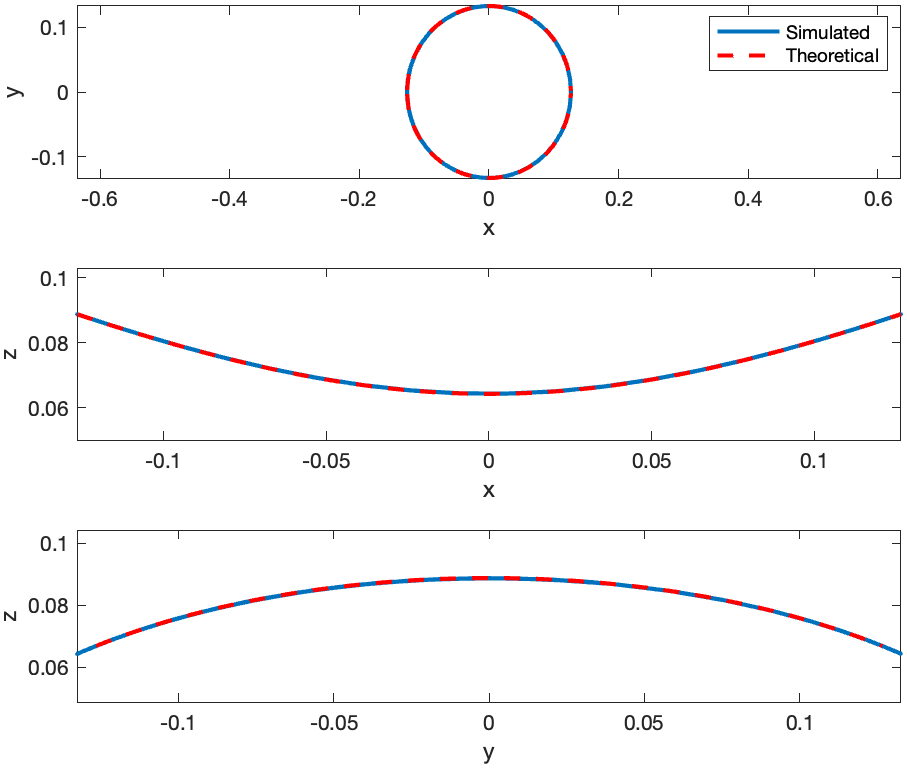
\includegraphics[width = 10cm]{Images/planar_polhode_random.png}
    \caption{Polhode Curve Projected onto Principally Aligned Cartesian Coordinate Planes}
    \label{fig:2d_polhode}
\end{figure}

\subsubsection{Repeat above steps changing initial conditions, e.g. setting angular velocity vector parallel to principal axis. Is the behavior according to expectations?} \label{sec:principally_aligned_omega}

Now with an initial condition of $\vec{\omega}_0 = \begin{bmatrix}
    10 & 0 & 0
\end{bmatrix}^T {}^{\circ}/s$ the magnitude of momentum and kinetic energy are 3056.1 kg m/s and 266.69 J respectively. With the angular velocity vector strictly aligned with one of the principal axes, the vector does not evolve in the principally oriented frame. That is, there is no gyroscopic coupling that causes the zero components of the angular velocity to increase or decrease. The vector components plotted over time are seen in Figure \ref{fig:sim_omegas_principal} 

\begin{figure}[H]
    \centering
    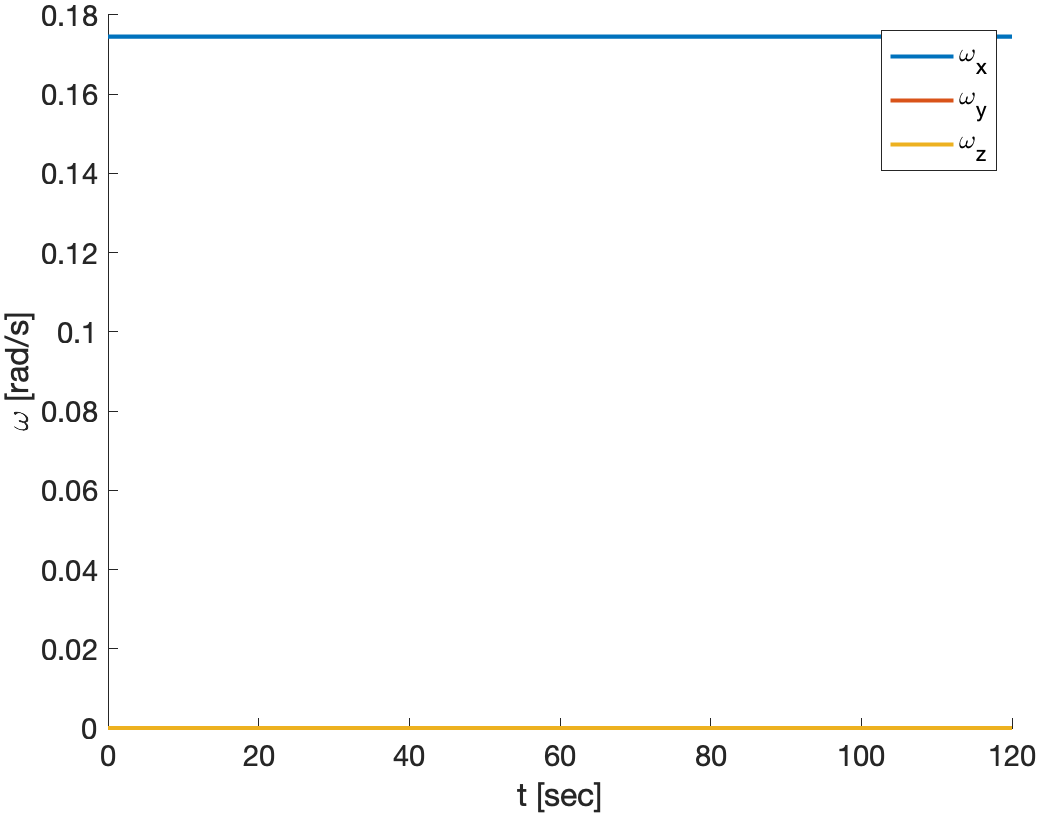
\includegraphics[width = 10cm]{Images/omega_prop_principal.png}
    \caption{Angular Velocity Vector Components for Principally Aligned Initical Conditions}
    \label{fig:sim_omegas_principal}
\end{figure}

The momentum and energy ellipsoids along with their semi-axis lengths can be seen plotted in Figures \ref{fig:momentum_axis_verification_princ} and \ref{fig:energy_axis_verification_princ} respectively.

\begin{figure}[H]
    \centering
    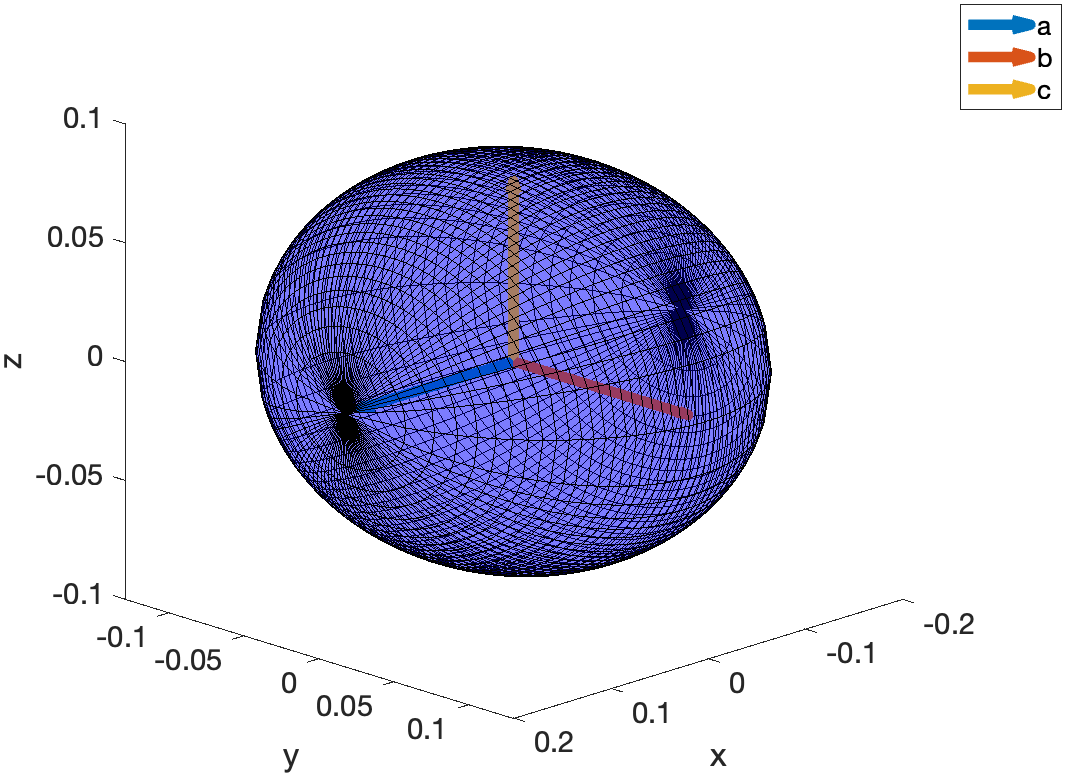
\includegraphics[width = 10cm]{Images/momentum_axes_principal.png}
    \caption{Momentum Ellipsoid and Semi-Axis Lengths for Principally Aligned Velocity Vector}
    \label{fig:momentum_axis_verification_princ}
\end{figure}

\begin{figure}[H]
    \centering
    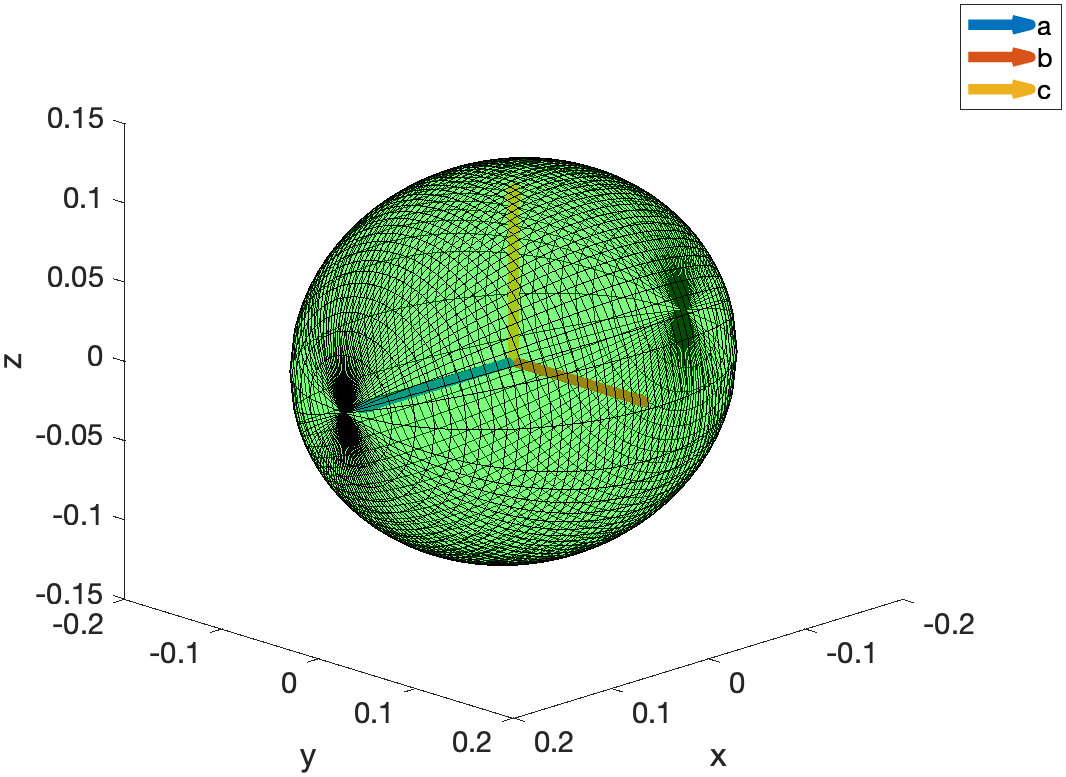
\includegraphics[width = 10cm]{Images/energy_axes_principal.png}
    \caption{Energy Ellipsoid and Semi-Axis Lengths for Principally Aligned Velocity Vector}
    \label{fig:energy_axis_verification_princ}
\end{figure}

This manifests in the polhode graph being a single point. Figure \ref{fig:ellipsoid_super_plot_principal} shows this point plotted at the intersection of the energy and momentum ellipsoids. The intersection in this case is strictly a point as the momentum ellipsoid is fully contained within the energy ellipsoid with two tangent points at  $10^{\circ}/s$ and $-10{}^{\circ}/s$ along the x-axis. 

\begin{figure}[H]
    \centering
    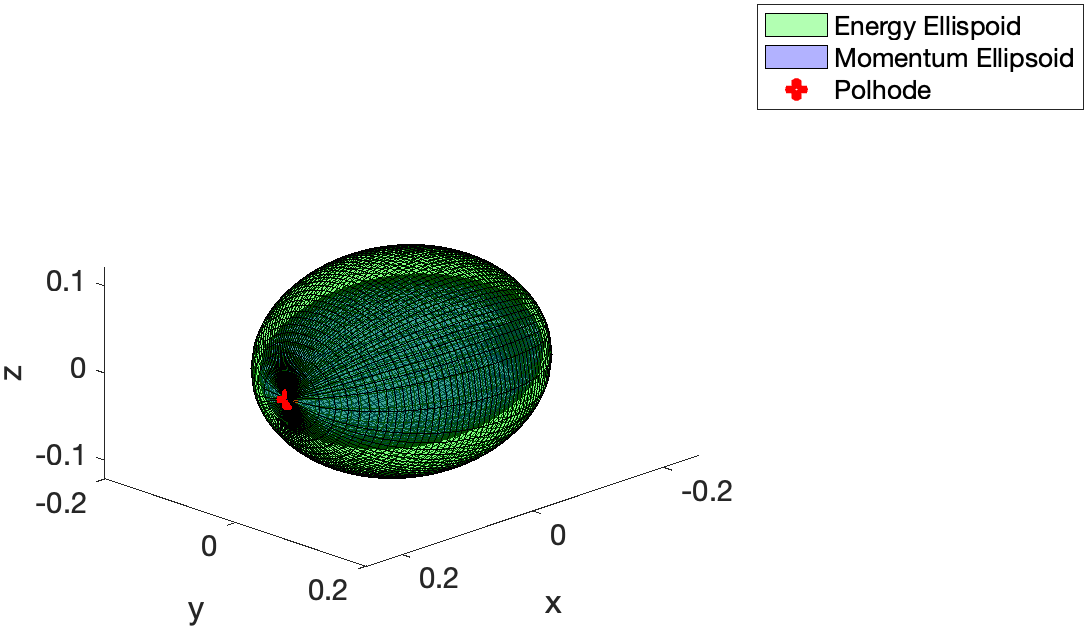
\includegraphics[width = 12cm] {Images/ellipsoid_polhode_principal.png}
    \caption{Momentum and Energy Ellipsoids and Polhode for Angular Velocity Aligned with a Principal Axis}
    \label{fig:ellipsoid_super_plot_principal}
\end{figure}

The polhode projected onto 2D axes is a single point that should lie along the theoretical curve described in Equations \ref{eq:polhode1}, \ref{eq:polhode2}, and \ref{eq:polhode3}. This is shown to hold true in Figure \ref{fig:2d_polhode_principal}. The points from simulation are seen to coincide with the theoretical expectation within an error on the order of magnitude of $10^{-8}$. Additionally, with these initial conditions, the quantity $L^2/2T$ evaluates to 17510 kg m\textsuperscript{2} which lies within the specified bounds described in \ref{sec:principal_inertia_def_and_calc}..

\begin{figure}[H]
    \centering
    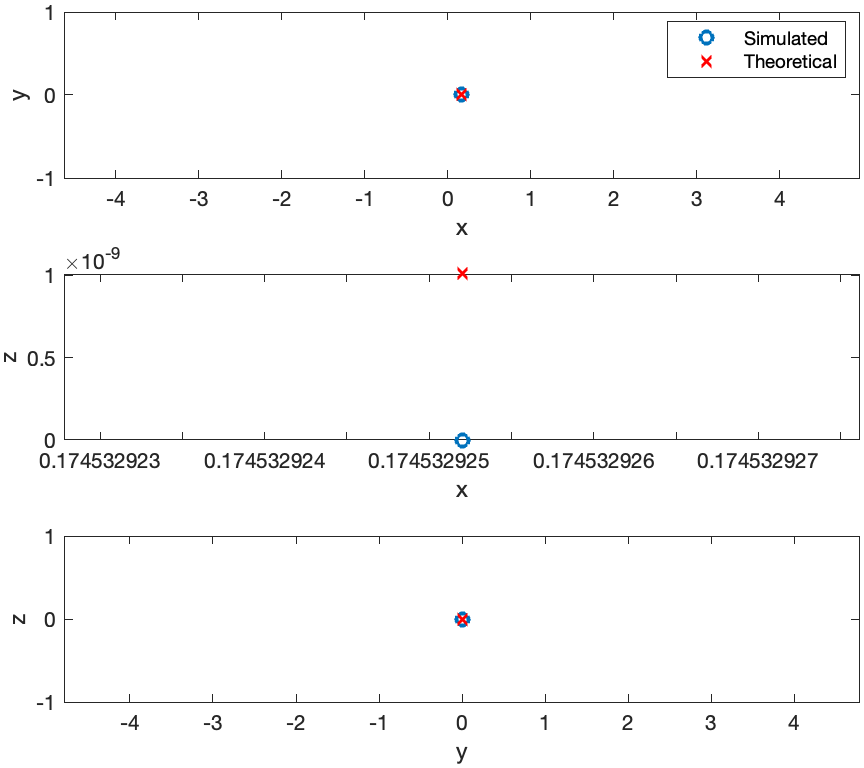
\includegraphics[width = 10cm]{Images/planar_polhode_principal.png}
    \caption{Projected Polhode Curve for Principally Aligned Angular Velocity Vector}
    \label{fig:2d_polhode_principal}
\end{figure}

The code used to perform all calculations and plots for Sections \ref{sec:principal_inertia_def_and_calc} -- \ref{sec:principally_aligned_omega} is listed below.

\lstinputlisting{Code/HW2main.m}
\section{\Large PROBLEM SET 3}
\subsection{Problem 3}

\subsubsection{Impose that satellite is axial-symmetric (i.e., impose $I_x=I_y\neq I_z$). Repeat numerical simulation from previous pset using initial condition 4) from previous pset.}

The principal inertia of the Aqua satellite is listed in \ref{sec:principal_inertia_def_and_calc}. Imposing that $I_y=I_x$, the axis-symmetric representation of the satellite is seen below.



\subsubsection{Program analytical solution for axial-symmetric satellite. Compute it at same time steps and from same initial conditions.}

\subsubsection{Compare numerical and analytical solutions. Plot differences (errors), do not only superimpose absolute values. Tune numerical integrator for large discrepancies. Are angular velocity vector and angular momentum vector changing according to theory in principal axes?}

\subsubsection{Program Kinematic equations of motion correspondent to a nominal attitude parameterization of your choice.}

\subsubsection{Program Kinematic equations of motion correspondent to a different attitude parameterization from the previous step. This is used for comparison, to get familiar with different approaches, and as fall back solution in the case of singularities.}

\subsubsection{Go back to your original satellite inertia tensor. Numerically integrate Euler AND Kinematic equations from arbitrary initial conditions (warning: stay far from singularity of adopted parameterization). Multiple revolutions. The output is the evolution of the attitude parameters over time. These attitude parameters describe orientation of principal axes relative to inertial axes.}

\subsubsection{Since inertial position, velocity, and attitude, are known at the same time throughout the simulation, it is now possible to express vectors in the reference systems of interest}
\section{\Large PROBLEM SET 4}

\subsection{Problem 1 - Equilibrium Tests}

\subsubsection{Assume that 2 components of the initial angular velocities are zero, and that the principal axes are
aligned with the inertial frame (e.g., zero Euler angles). Verify that during the simulation the 2
components of angular velocity remain zero, and that the attitude represents a pure rotation about
the rotation axis (e.g., linearly increasing Euler angle). Plot velocities and angles.}

\subsubsection{Repeat a. by setting the initial attitude to match the RTN frame. Set the initial angular velocity to
be non-zero only about N. Show the evolution of attitude motion in the RTN frame and give an
interpretation of the results (recall that you might have J2 effects in orbit propagation, consider
removing them for verification).}

\subsection{Problem 2 - Stability Tests}

\subsubsection{Pretend you have a single-spin satellite. Set initial conditions to correspond alternatively to the 3
possible equilibrium configurations (rotation about principal axes of inertia). Slightly perturb initial
condition. Is the attitude stable or unstable? In angles and velocities? If stable, periodically or
asymptotically? Show it.}

\subsection{Problem 3 - Adding a Momentum Wheel or Rotor (Dual-Spin Satellite)}

\subsubsection{Re-program Euler equations to include a generic momentum wheel or rotor with rotation axis
aligned with one of the principal axes of inertia. Ideally the wheel or rotor has specs representative
of commercial products (inertia, rotational speed).}

\subsubsection{Numerically integrate Euler AND Kinematic equations from equilibrium initial condition. Verify
that integration is correct as from previous tests (conservation laws, rotations, etc.).}

\subsubsection{Verify equilibrium and its stability similar to previous pset.}

\subsubsection{Use the stability condition to make attitude motion stable for rotation about intermediate moment
of inertia by changing moment of inertia and/or angular velocity of the momentum wheel or rotor.}

\subsubsection{Try to make rotation about another arbitrary axis (potentially relevant to your project) stable
through a generic momentum wheel or rotor.}

\subsection{Problem 4 - Gravity Gradient Torque (Modeling)}

\subsubsection{Remove rotor.}

\subsubsection{Program gravity gradient torque. Feed torque to Euler equations. This is the first perturbation you
model resulting from the interaction of the spacecraft with the environment. Hint: change your orbit
to make gravity gradient significant if that’s not the case.}

\subsubsection{Verify that the magnitude of the modelled torque is consistent with the orbit and inertia tensor of
your satellite. Hint: use simplified formulas from class on modelling of gravity gradient torque.}

\subsubsection{Numerically integrate Euler and Kinematic equations including gravity gradient from initial
conditions corresponding to body axes aligned with the orbital frame (RTN). Verify that gravity
gradient torque is zero, besides numerical errors. Hint: you may need to simplify the orbit to
unperturbed circular to achieve this. Check that initial angular velocity matches mean motion.}

\subsubsection{Numerically integrate Euler and Kinematic equations including gravity gradient from arbitrary
initial conditions (e.g., relevant to your project). Plot external torque (3 components w.r.t. time)
and resulting attitude motion (depends on attitude parameterization, add Euler angles for better
geometrical interpretation) over multiple orbits. Comment on results.}



\section{\Large PROBLEM SET 5}

\subsection{Problem 1 - Gravity Gradient Torque (Stability)}

\subsubsection{Calculate the coefficients Ki of the moments of inertia which drive stability under gravity gradient. Compute and plot regions of stable and unstable motion.}

Using Demos, an online graphing calculator tool, the plot shown in Figure \ref{fig:grav_gradient_stability} was produced. As shown in annotations on the figure, this plot represents regions in the $k_Tk_R$ plane for which stability is achieved. The equilibrium point about which this stability is described is one in which the principal axes of the spacecraft are aligned with the RTN frame, and the angular velocity of the spacecraft expressed in the principal frame is $\vec{\omega} = \begin{bmatrix} 0 & 0 & n \end{bmatrix}^T$, where $n$ is the mean motion of the spacecraft in its orbit. 

\begin{figure}[H]
    \centering
    \captionsetup{ justification = centering}
    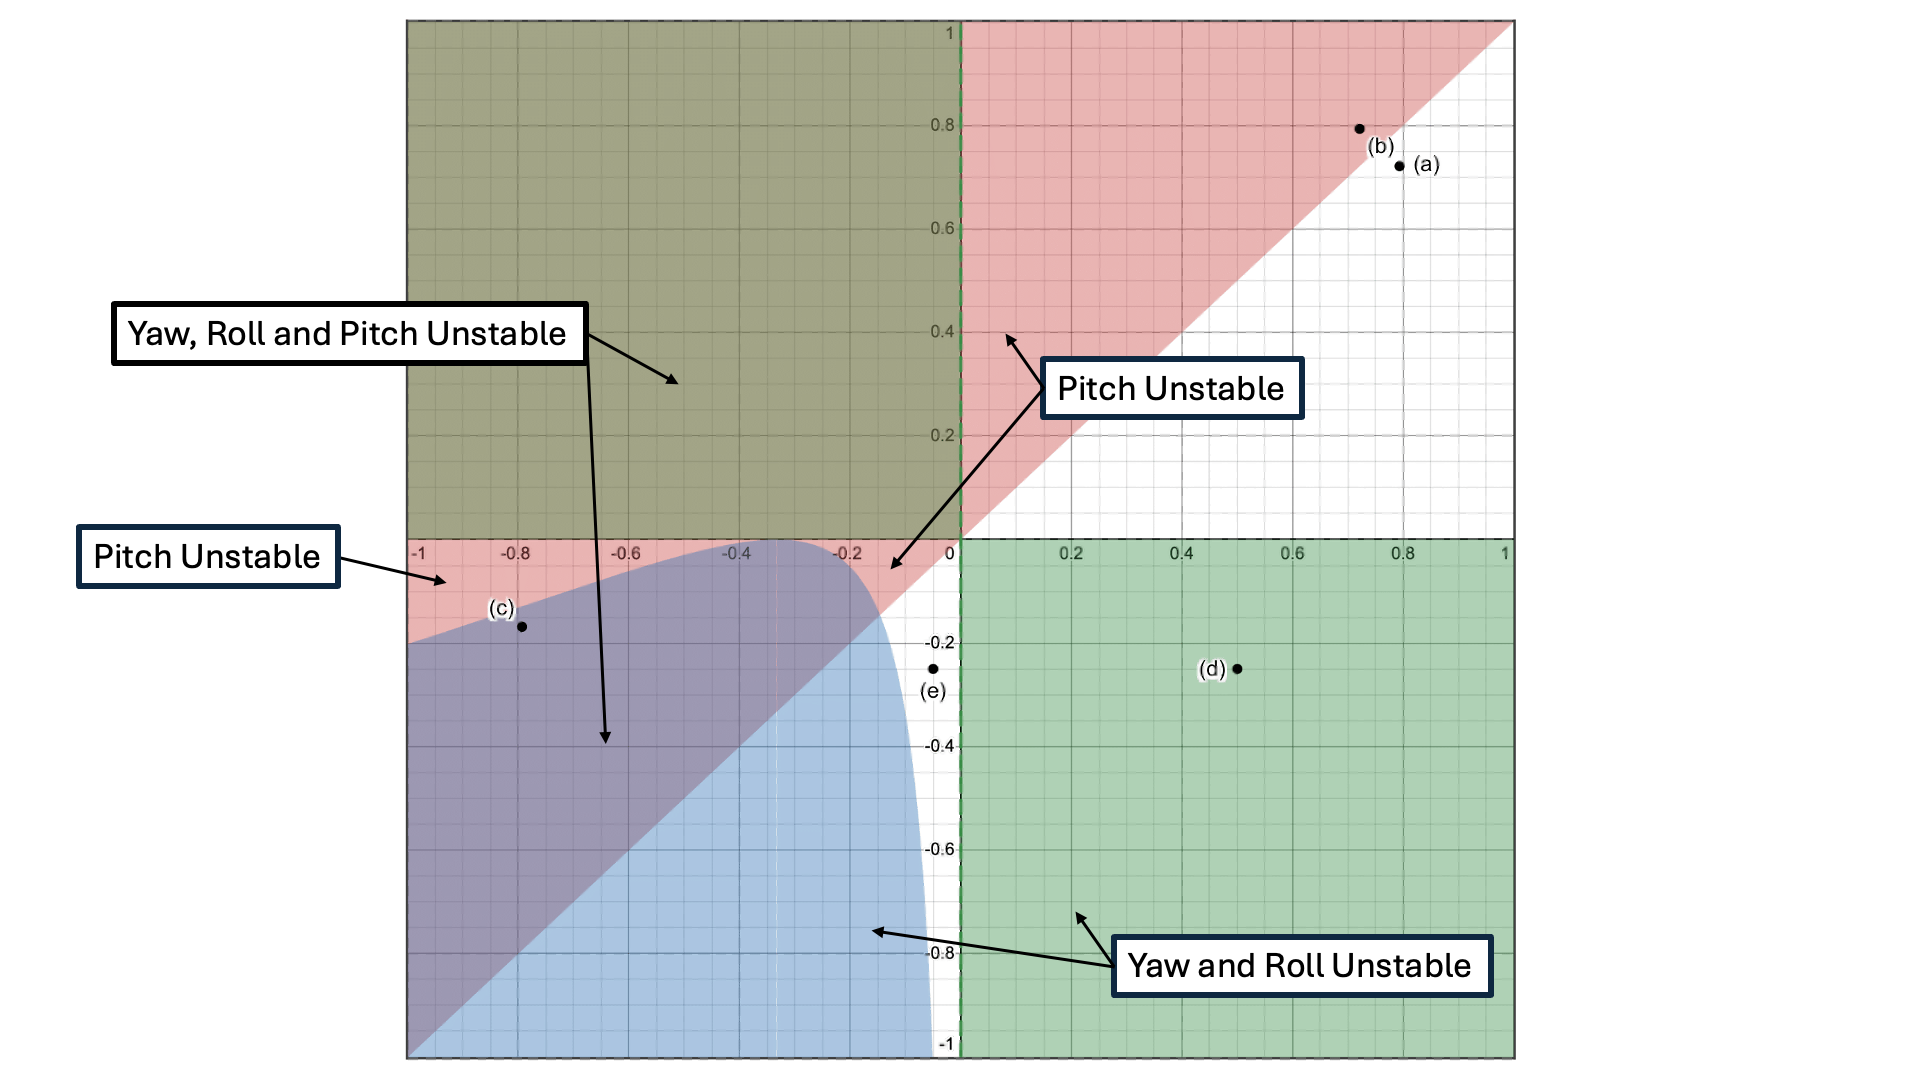
\includegraphics[width = 15cm]{Images/PS5/gravityGradientStabilityPlot.png}
    \caption{Plot of Stability Regions in the $k_Tk_R$ Plane with Various Simulated Test Points which Describe Several States of Stability and Instability}
    \label{fig:grav_gradient_stability}
\end{figure}

The definitions of $k_N$, $k_T$, and $k_R$ are seen in Equations \ref{eq:k_N}, \ref{eq:k_T}, and \ref{eq:k_R} respectively. 

\begin{eqnarray}
    k_N &= \frac{I_y - I_x}{I_z} \label{eq:k_N} \\
    k_T &= \frac{I_z - I_x}{I_y} \label{eq:k_T} \\
    k_R &= \frac{I_z - I_y}{I_x} \label{eq:k_R}
\end{eqnarray}

\subsubsection{Considering the results from 1a, comments on the expected stability of the attitude motion of your satellite about equilibrium. Try to reproduce stable and unstable motion by setting proper initial conditions and perturbing those conditions slightly (e.g., by 1\%). Plot attitude parameters (e.g., Euler angles) to show stability or instability}

There are five points indicated in Figure \ref{fig:grav_gradient_stability}, the coordinates of which are shown in Table \ref{tab:k_plane_points} along with the respective principal inertia values that yield the listed configurations.

\begin{table}[H]
    \centering
    \captionsetup{justification = centering}
    \begin{tabular}{c|ccccc}
    Point  & $k_T$ & $k_R$ & $I_{xx}$ [kg m\textsuperscript{2}] & $I_{yy}$ [kg m\textsuperscript{2}] & $I_{zz}$ [kg m\textsuperscript{2}] \\ \hline
    a &   0.7933     &   0.7212    &   17510    &   23616    &  36245 \\
    b &   0.7212     &  0.7993     &   23616    &   17510    &  36245  \\  
    c &   -0.7933     &  -0.1685     &   36245    &   23616    &  17510  \\ 
    d &   0.5000     &  -0.2500     &   16109    &   40272    &  36245  \\ 
    e &   -0.0500     &  -0.2500     &   38539    &   45879    &  36245  \\ 
    \end{tabular}
    \caption{Test Points in $k_Tk_R$ Plane for Various Stability and Instability Conditions}
    \label{tab:k_plane_points}
\end{table}

The point that corresponds to Aqua's nominal configuration is Point (a). It can be seen that this lies in a stable (unshaded) region in the first quadrant of Figure \ref{fig:grav_gradient_stability}. Initializing the simulation with the the velocities and Euler angles slightly perturbed from the equilibrium state described above, the stability can be verified in simulation. Figure \ref{fig:point_a_grav_stability} shows a time history of the velocities, the Euler angles describing rotation between the principal and RTN frames, and lastly the components of the gravity gradient induced moment expressed in the principal frame. 

\begin{figure}[H]
    \centering
    \captionsetup{justification = centering}
    \includegraphics[width = 12cm]{Images/PS5/}
    \caption{Time History of Perturbed Equilibrium for Point (a)}
    \label{fig:point_a_grav_stability}
\end{figure}

Points (b)--(d) describe unstable conditions along various axes. The following plots (Figures \ref{point_b_grav_stability}--\ref{point_d_grav_stability} shows the same stability analysis performed for these points.

\begin{figure}[H]
    \centering
    \captionsetup{justification = centering}
    \includegraphics[width = 12cm]{Images/PS5/}
    \caption{Time History of Perturbed Equilibrium for Point (b)}
    \label{fig:point_b_grav_stability}
\end{figure}

\begin{figure}[H]
    \centering
    \captionsetup{justification = centering}
    \includegraphics[width = 12cm]{Images/PS5/}
    \caption{Time History of Perturbed Equilibrium for Point (c)}
    \label{fig:point_c_grav_stability}
\end{figure}

\begin{figure}[H]
    \centering
    \captionsetup{justification = centering}
    \includegraphics[width = 12cm]{Images/PS5/}
    \caption{Time History of Perturbed Equilibrium for Point (d)}
    \label{fig:point_d_grav_stability}
\end{figure}

Through the analysis of Figure \ref{fig:grav_gradient_stability}, Point (b) is predicted to be unstable strictly in pitch. 

Point (c), however, is predicted to be unstable in yaw, pitch, and roll.

Lastly, Point (d) is expected to be yaw and roll unstable while still stable in pitch.

Another stable condition where the spacecraft is spinning about the minimum inertia is corresponds to Point (e). The stability behavior of this satellite is seen in Figure \ref{fig:point_e_grav_stability}.

\begin{figure}[H]
    \centering
    \captionsetup{justification = centering}
    \includegraphics[width = 12cm]{Images/PS5/}
    \caption{Time History of Perturbed Equilibrium for Point (e)}
    \label{fig:point_e_grav_stability}
\end{figure}

\subsubsection{How would you need to change the mass distribution and/or nominal attitude of your satellite to obtain stable motion from the gravity gradient torque? Would it make sense for your project? Show a couple of potential configurations in the Ki plane and resulting stability of attitude motion at the equilibrium. This is done by changing your inertia tensor and simulating numerically}

The spacecraft is already stable about the equilibrium described above, however it might make sense to find an equilibrium such that the spacecraft is spinning about its minimum inertia. This would ensure that the craft was already in its lowest energy state, so any unmodeled dissipation would not result in the orientation of the spacecraft changing. Very fortunately, the minimum axis of inertia for the nominal Aqua model (i.e. the x-axis in the current principal frame) is closely aligned with the y-axis in the body frame. An Earth pointing orientation for this mission is synonymous with this axis being aligned with the N-axis in the RTN frame. Therefore, it would make sense to achieve stable equilibrium about this axis. The stability of the spacecraft in this orientation will be investigated in the future.

\subsection{In addition to gravity gradient, start programming perturbation torques due to magnetic field, solar radiation pressure, and atmospheric drag.}

To create a simple, early use model for the magnetic disturbance torques, the Earth is modeled as a magnetic dipole. This assumption is not accurate for LEO, but will give helpful insight to how the spacecraft motion will be affected by this disturbance along with the ability to size actuators. A more accurate model will be investigated in the future. 
When modeling the magnetic dipole of the spacecraft, a major simplification was made. The spacecraft was split into two main components---the chassis along and instruments as one component with the solar panel as another. Each component is modeled as a insulating cylinder with an electromagnetic coil wrapped around it. The model for the dipole moment created by each of these components is described in Equation \ref{eq:spacecraft_dipole}, where $\mu_0$ is the permeability of vacuum, $S$ is the surface area between each coil, $n$ is the number of coils, and $\Delta I$ is the variable current passing through the coil. For the current state of the model, these numbers were chosen very arbitrarily. They are reported in Table \ref{tab:spacecraft_dipole_data} along with the direction and magnitude of the resulting dipole moment.

This approximation of the disturbance was implemented using the Simulink model depicted in Figure \ref{fig:simulink_mag}.
\section{\Large PROBLEM SET 6}

\subsection{Problem 1 - Complete the modeling and verification of perturbation torques as described in the previous pset} \label{sec:pertTorques}

In the previous problem set, the magnetic torque was implemented successfully, but the aerodynamic and solar radiation torques still needed improvement. For the solar radiation torque, the unit vector pointing towards the sun needed to be implemented. To accomplish this, the orbit propagator used for the satellite was leveraged. The propagator was modified to take in the orbital elements of the desired orbit at the beginning of the simulation such that it could be called separately for the satellite and the sun. The new resultant layout of the simulink file is shown below in Figure \ref{fig:sun_orbit_sim}.

\begin{figure}[H]
    \centering
    \captionsetup{ justification = centering }
    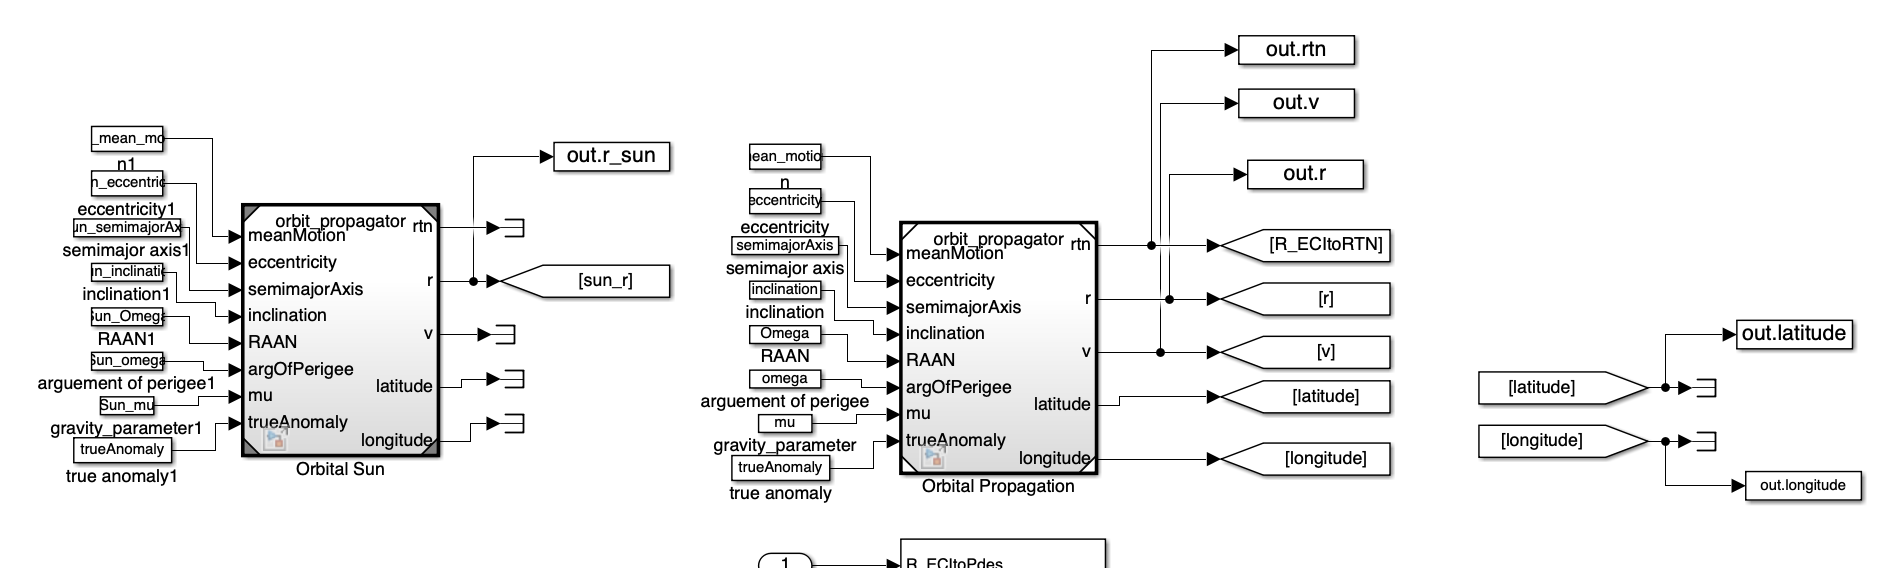
\includegraphics[width = 12cm]{Images/PS6/updatedOrbitPropagatorSim.png}
    \caption{Updated Orbit Propagator to include Sun Orbit Propagation}
    \label{fig:sun_orbit_sim}
\end{figure}

In the above simulink model, the orbital elements of Earth's orbit around the sun were used to simulate the 'orbit' of the sun around the Earth in the ECI frame. The semimajor axis and eccentricity were left untouched as they are independent of coordinate frames. It is important to note, however, that the angular values including the inclination were adjusted to be in Earth's equatorial plane that is offset by the ecliptic plane by 23.5$\degree$. The orbital parameters that were used are shown below.

\begin{center}
    a = 7080.6 km \\
    e = 0.0000979 \\
    i = 98.2$\degree$ \\
    $\Omega$ = 95.2063$\degree$ \\
    $\omega$ = 120.4799$\degree$ \\
\end{center}

A plot showing the resultant orbit of the sun 'around' the Earth is shown below in Figure \ref{fig:sun_orbit}.

\begin{figure}[H]
    \centering
    \captionsetup{ justification = centering }
    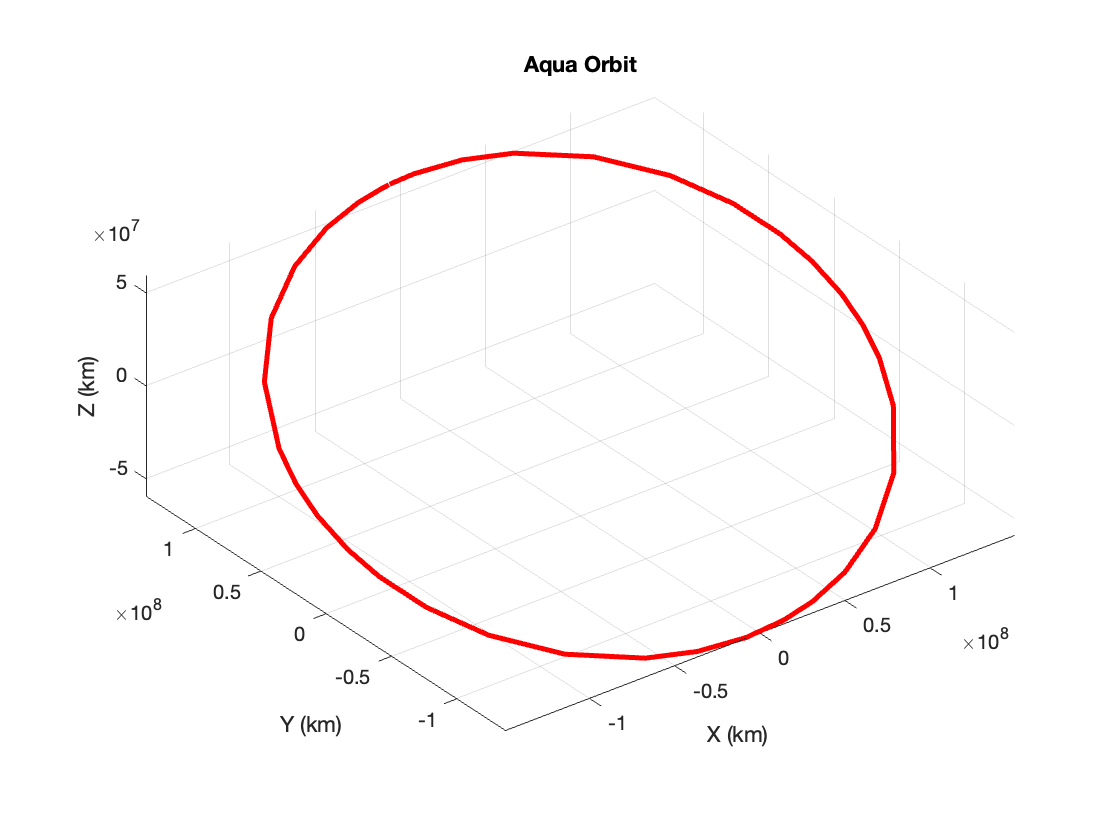
\includegraphics[width = 12cm]{Images/PS6/sunOrbit.png}
    \caption{Orbit of the Sun Around Earth in ECI Frame}
    \label{fig:sun_orbit}
\end{figure}

One it was verified that the unit vector pointing towards the sun was correct, the remaining tasks for the solar radiation torque were finding values for $c_d$ and $c_s$ that aligned with the theory and approximating the center of pressure of the satellite. While the exact materials used for the Aqua satellite are unknown, it is safe to assume that the solar array had a lower $c_d$ value than the encasing of the sensors and electronics in the satellite. This is because the encasing is typically covered in an opaque white paint to protect the electronics from environmental dangers. Therefore, $c_d$ was adjusted to be high for every surface except the two designated to the solar array and $c_1$ followed the opposite relationship to ensure that $c_d + c_s < 1$. Finally, the center of pressure was calculated through the following approximation.

\begin{equation}
    \frac{\sum^n_{i=1} A_i c_i}{\sum^n_{i=1} A_i}
\end{equation}

In this equation A represents the area of each surface and c represents the centroid location in the principle frames. Through making these corrections and debugging small issues in the simulink model shown in Figure \ref{fig:simulink_sol}. The resultant torques plotted versus time are shown in Figure \ref{fig:solar_torque}.

\begin{figure}[H]
    \centering
    \captionsetup{ justification = centering }
    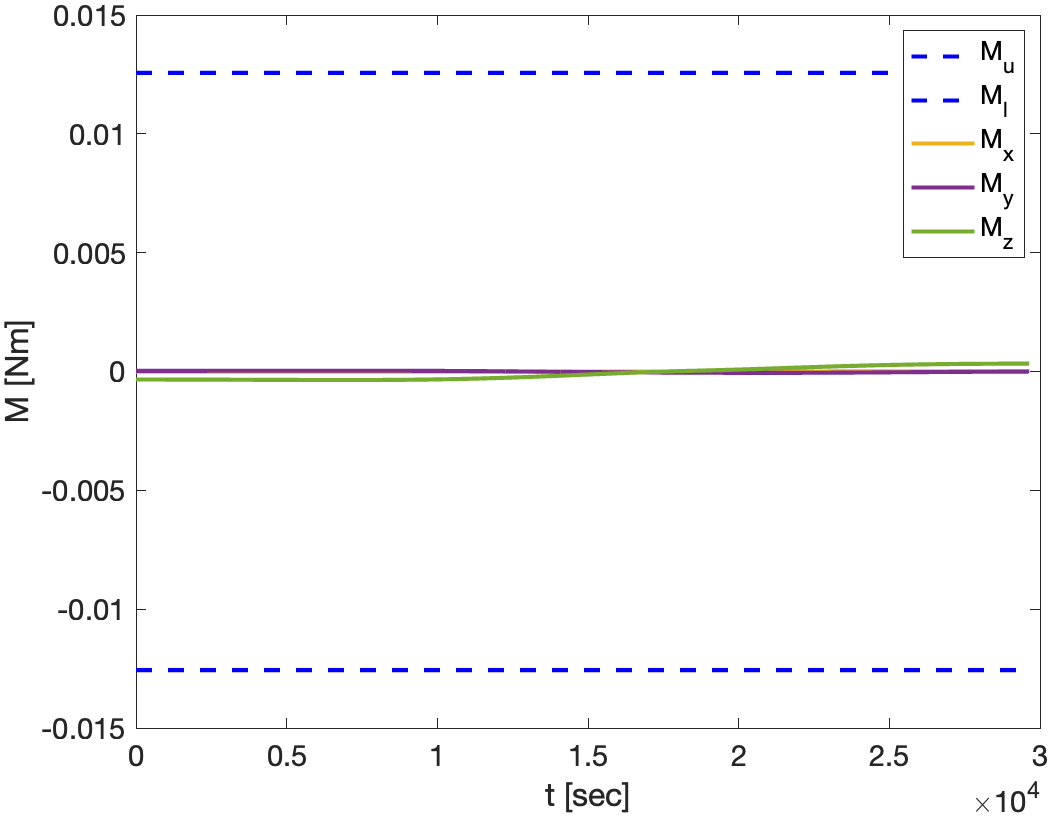
\includegraphics[width = 12cm]{Images/PS6/solar_torque.png}
    \caption{Solar Torque}
    \label{fig:solar_torque}
\end{figure}

The small oscillations shown in Figure \ref{fig:solar_torque} confirm that the torque is periodic for the Earth pointing satellite as predicted in theory. Furthermore, the torque is well within the bounds. 

For the aerodynamic drag, the theory shown in last weeks problem set was correct, but small issues needed to be debugged with the model. Once these bugs were resolved, the resultant torques were obtained and are shown below in Figure \ref{fig:aero_torque}.

\begin{figure}[H]
    \centering
    \captionsetup{ justification = centering }
    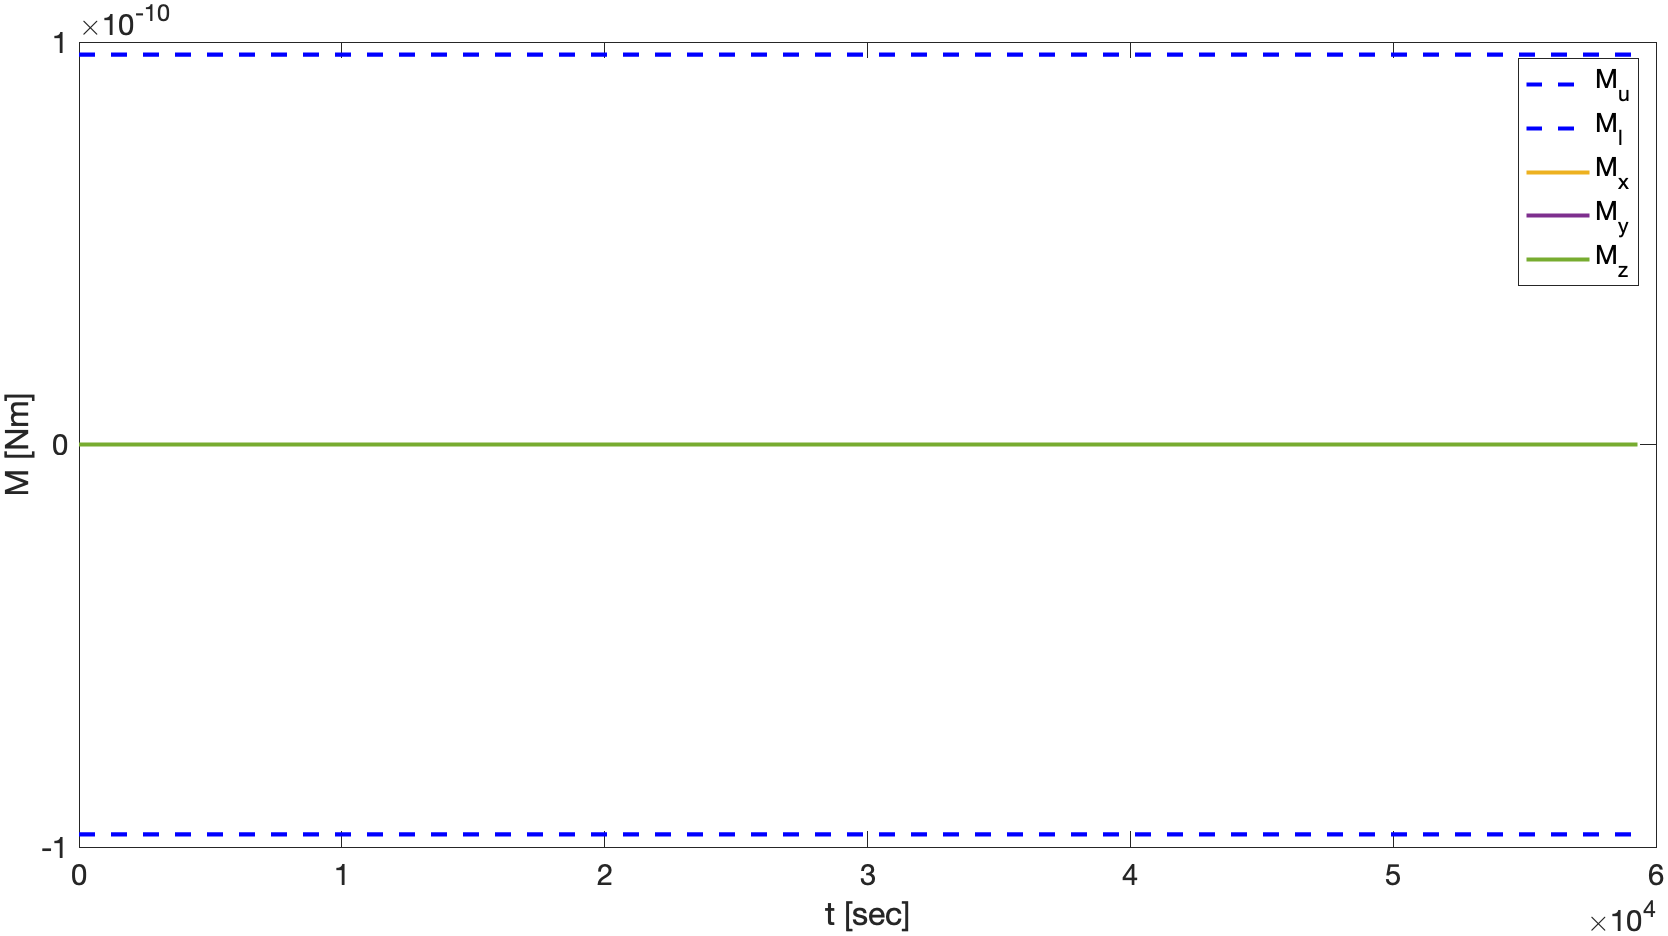
\includegraphics[width = 12cm]{Images/PS6/aero_torque.png}
    \caption{Aerodynamic Torque}
    \label{fig:aero_torque}
\end{figure}


As predicted in the theory, the drag is constant for the earth pointing satellite, and stays well within the bounds thus validating the simulation. Finally, once all of the disturbances were obtained, they were combined to obtain the total torque from aerodynamic drag, solar radiation, gravity, and magnetic disturbances. The total torque is shown below in Figure \ref{fig:all_torque}.

\begin{figure}[H]
    \centering
    \captionsetup{ justification = centering }
    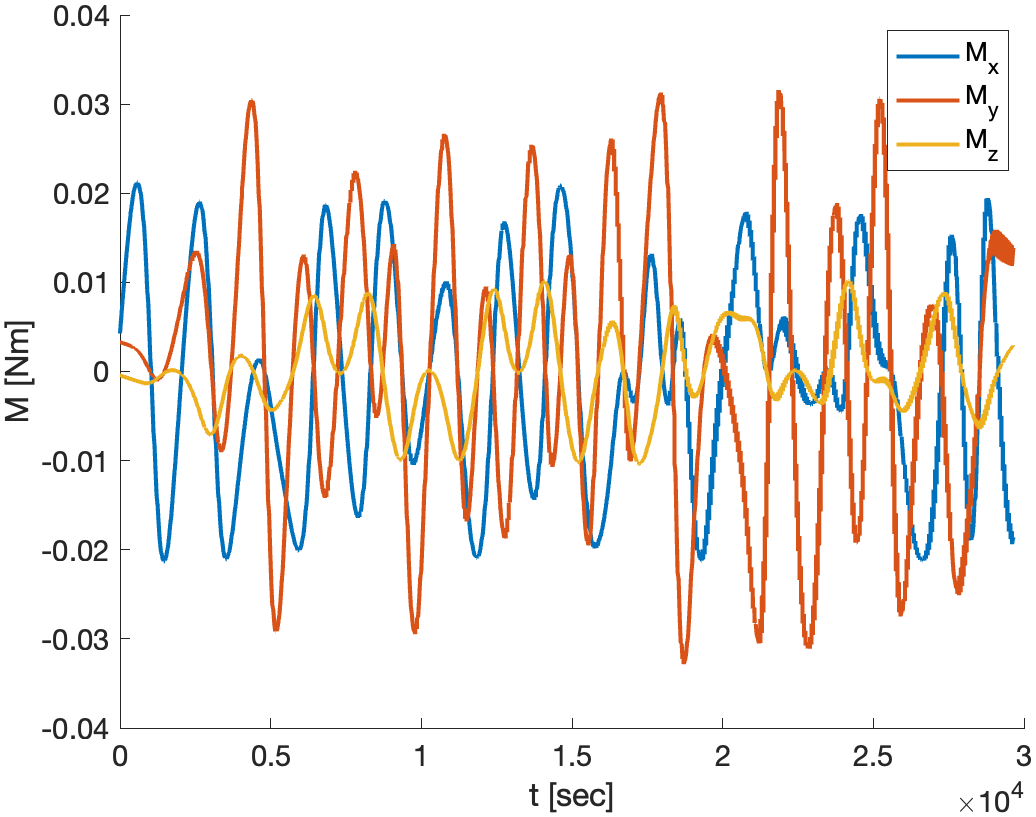
\includegraphics[width = 12cm]{Images/PS6/all_torque.png}
    \caption{Total Torque}
    \label{fig:all_torque}
\end{figure}

The total torque shows that the primary disturbance contributors are gravity and solar radiation for our satellite and its mission. 

\subsection{Problem 2 - Compute the attitude control error even if a controller is not implemented yet. The attitude control error represents the rotation between the desired and actual attitude. Plot the attitude control error and give its interpretation. Note that this step requires the definition and computation of the desired or nominal or target attitude of the spacecraft. In general, this can be expressed in body or principal axes.}

Recall that the mission for the Aqua satellite requires the instruments on the bottom of the spacecraft to be Earth-pointing. With the selected body axes, this means that the desired attitude expressed as a rotation matrix from the RTN frame to the body frame is described as follows.

\begin{equation*}
    \boldsymbol{\bar{R}}_{RTN \rightarrow x'y'z'} = \begin{bmatrix}
        0 & 1 & 0 \\ 0 & 0 & 1 \\ 1 & 0 & 0
    \end{bmatrix}
\end{equation*}

To get the desired orientation of the principal frame we use the rotation described in Section \ref{sec:principal_inertia_def_and_calc}. Using Equation \ref{eq:desired_principal_RTN}, the desired attitude of the principal frame with respect to the RTN frame can computed, where $\boldsymbol{A}$ is represented by $\boldsymbol{R}_{xyz \rightarrow x'y'z'}$.

\begin{equation} \label{eq:desired_principal_RTN}
    \boldsymbol{\bar{R}}_{RTN \rightarrow xyz} = \boldsymbol{R}_{xyz \rightarrow x'y'z'}^T \boldsymbol{\bar{R}}_{RTN \rightarrow x'y'z'}
\end{equation}

Therefore, at each step in the simulation, the desired attitude with respect to the ECI frame is computed using Equation \ref{eq:desired_principal_ECI}.

\begin{equation} \label{eq:desired_principal_ECI}
    \boldsymbol{\bar{R}}_{ECI \rightarrow xyz} = \boldsymbol{\bar{R}}_{RTN \rightarrow xyz} \boldsymbol{R}_{ECI \rightarrow RTN}
\end{equation}

The error between the current and desired attitude can be represented by a rotation from the current attitude to the desired attitude. This rotation can be computed using Equation \ref{eq:error_rotation}

\begin{equation} \label{eq:error_rotation}
    \boldsymbol{R}_{\text{error}} = \boldsymbol{R}_{xyz \rightarrow \overline{xyz}} = \boldsymbol{\bar{R}}_{ECI \rightarrow xyz} \boldsymbol{R}_{ECI \rightarrow xyz}^T
\end{equation}

Aligning the satellite initially with this initial condition but giving it no initial angular velocity should yield an evolution of the error that mostly resembles a linear increase in the angle $\theta$. This is because this angle represents the error about the desired 2-axis, which in our desired alignment corresponds to the N-axis in the RTN frame. In the absence of disturbances the only apparent rotation should be that of the RTN frame as the satellite moves in its orbit. Figure \ref{fig:attitude_error_no_dist} corroborates this interpretation. An issue occurs with a singularity at $\theta = 90^\circ$, causing the signs of the other two angles to flip. The general behavior, however, remains the same under this consideration.

\begin{figure}[H]
    \centering
    \captionsetup{ justification = centering }
    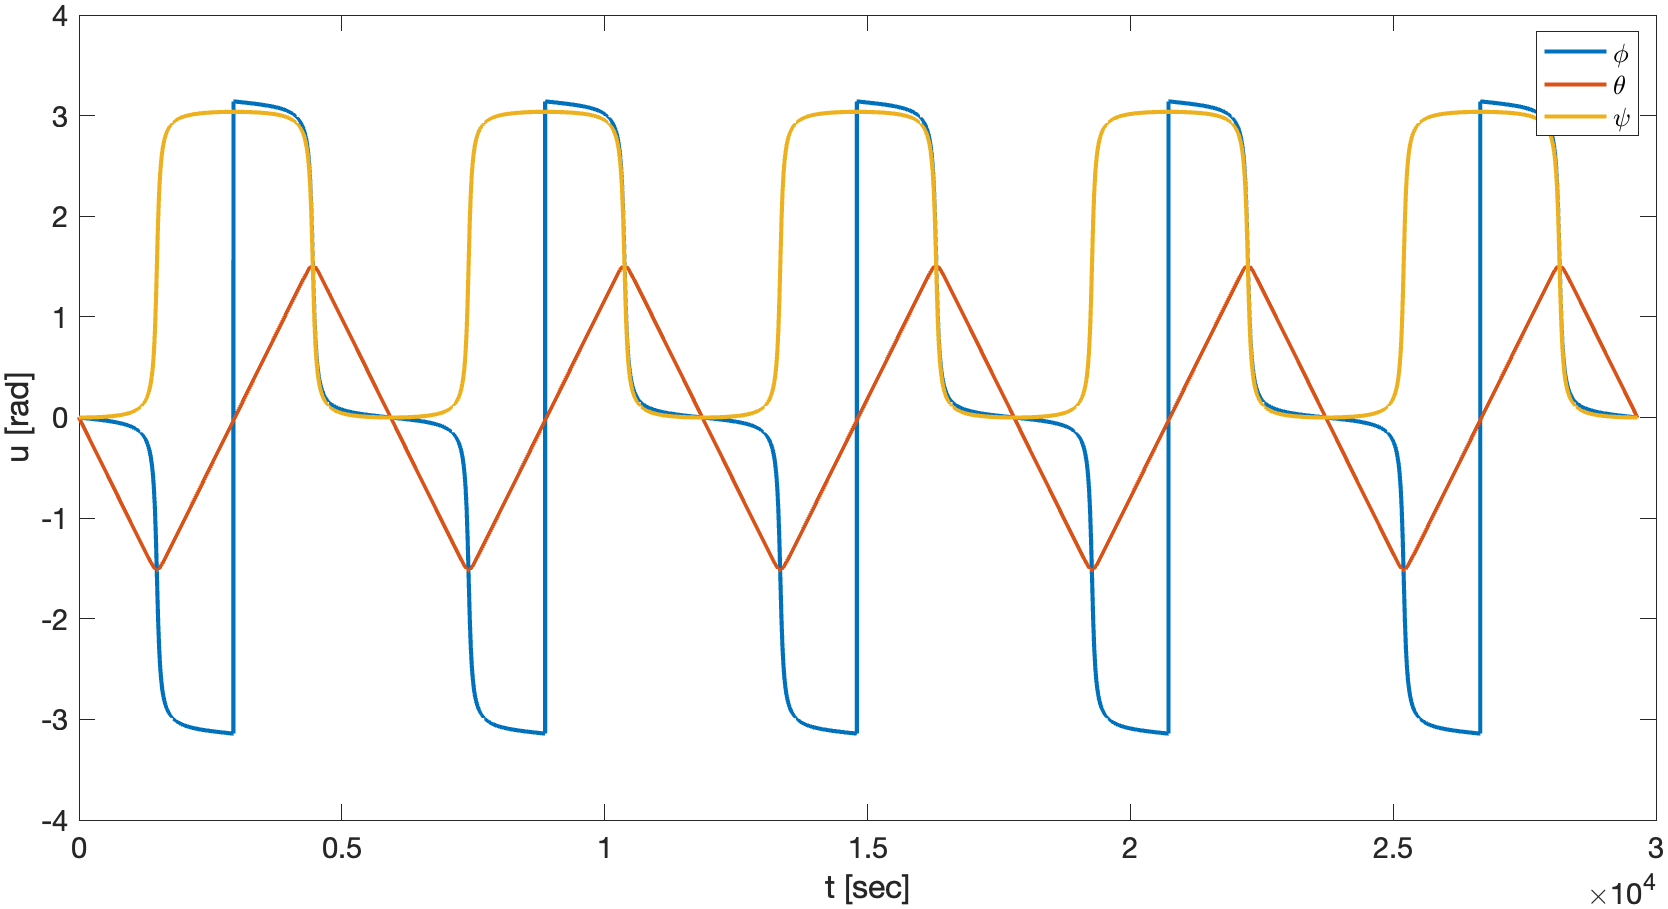
\includegraphics[width = 12cm]{Images/PS6/attitude_error_no_dist.png}
    \caption{312 Euler Angle Parameterization of the Rotation Error in the Absence of Disturbance Torques}
    \label{fig:attitude_error_no_dist}
\end{figure}

\subsection{Problem 3 - Note that the attitude control error represents a rotation matrix (DCM) which quantifies how far the actual attitude is from the true attitude. You can use any parameterization to plot the attitude control errors corresponding to this DCM. Give interpretation of the attitude control errors given the applied disturbances.}

In the presence of disturbances, the motion will be similar during a large portion of the first orbit, but the presence of oscillatory moments throughout each orbit will slowly change the angular velocity vector of the spacecraft, causing the evolution to become less linear and more oscillatory. The period of these oscillations will also grow shorter over time. The simulation results are shown in Figure \ref{fig:attitude_error_dist}.

\begin{figure}[H]
    \centering
    \captionsetup{ justification = centering }
    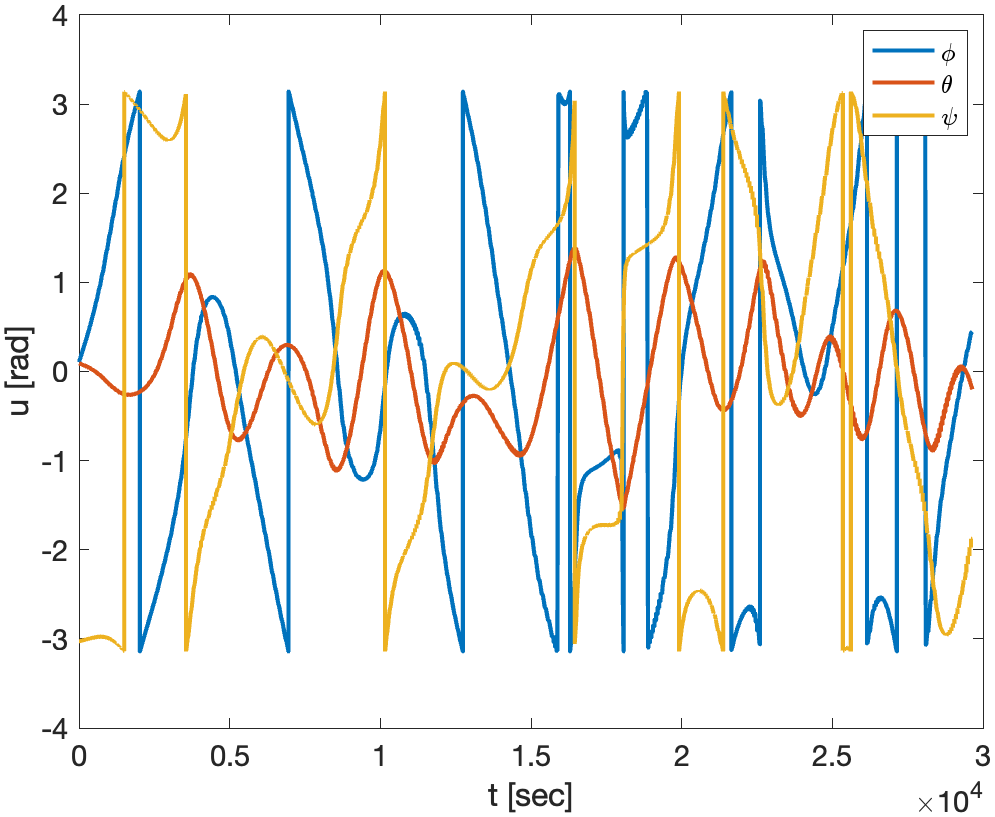
\includegraphics[width = 12cm]{Images/PS6/attitude_error_dist.png}
    \caption{312 Euler Angle Parameterization of the Rotation Error in Presence of Disturbance Torques}
    \label{fig:attitude_error_dist}
\end{figure}

\subsection{Problem 4 - You can now start modeling the Simulink spacecraft subsystem which is what the satellite believes is happening (on-board). Initially, the sensors provide ideal measurements (no bias or noise). Just use an empty box for those. The outputs of the sensors are measurements which are used for attitude determination. These measurements are computed from the reference truth or oracle.}

The sensors onboard the satellite that return reference vectors corresponding the location or direction of physical things in space are star trackers and magnetometers. For the sake of proving the functionality of the deterministic and statistical methods for attitude determination, it was deemed sufficient to only use star tracker measurements. 

The model shown in Figure \ref{fig:star_tracker_meas} depicts the simulated generation of star tracker measurements from a set of randomly selected ground truth unit vectors. In later test cases it will be seen that two sets of such random vectors were generated. One consists only of two ground truth vectors whereas the other consists of 10. The weights associated with these measurements are randomly generated as well, as there is no noise present in this validation stage. Once noise is present, the weights will be chosen much more carefully, especially in the presence of other sensors (e.g. magnetometers). To emulate noise, each component of the measurement vectors are perturbed by a random number ranging from -1 to 1 that is scaled by a so called "noise factor." Here, this factor is chosen to be 0.

\begin{figure}[H]
    \centering
    \captionsetup{ justification = centering }
    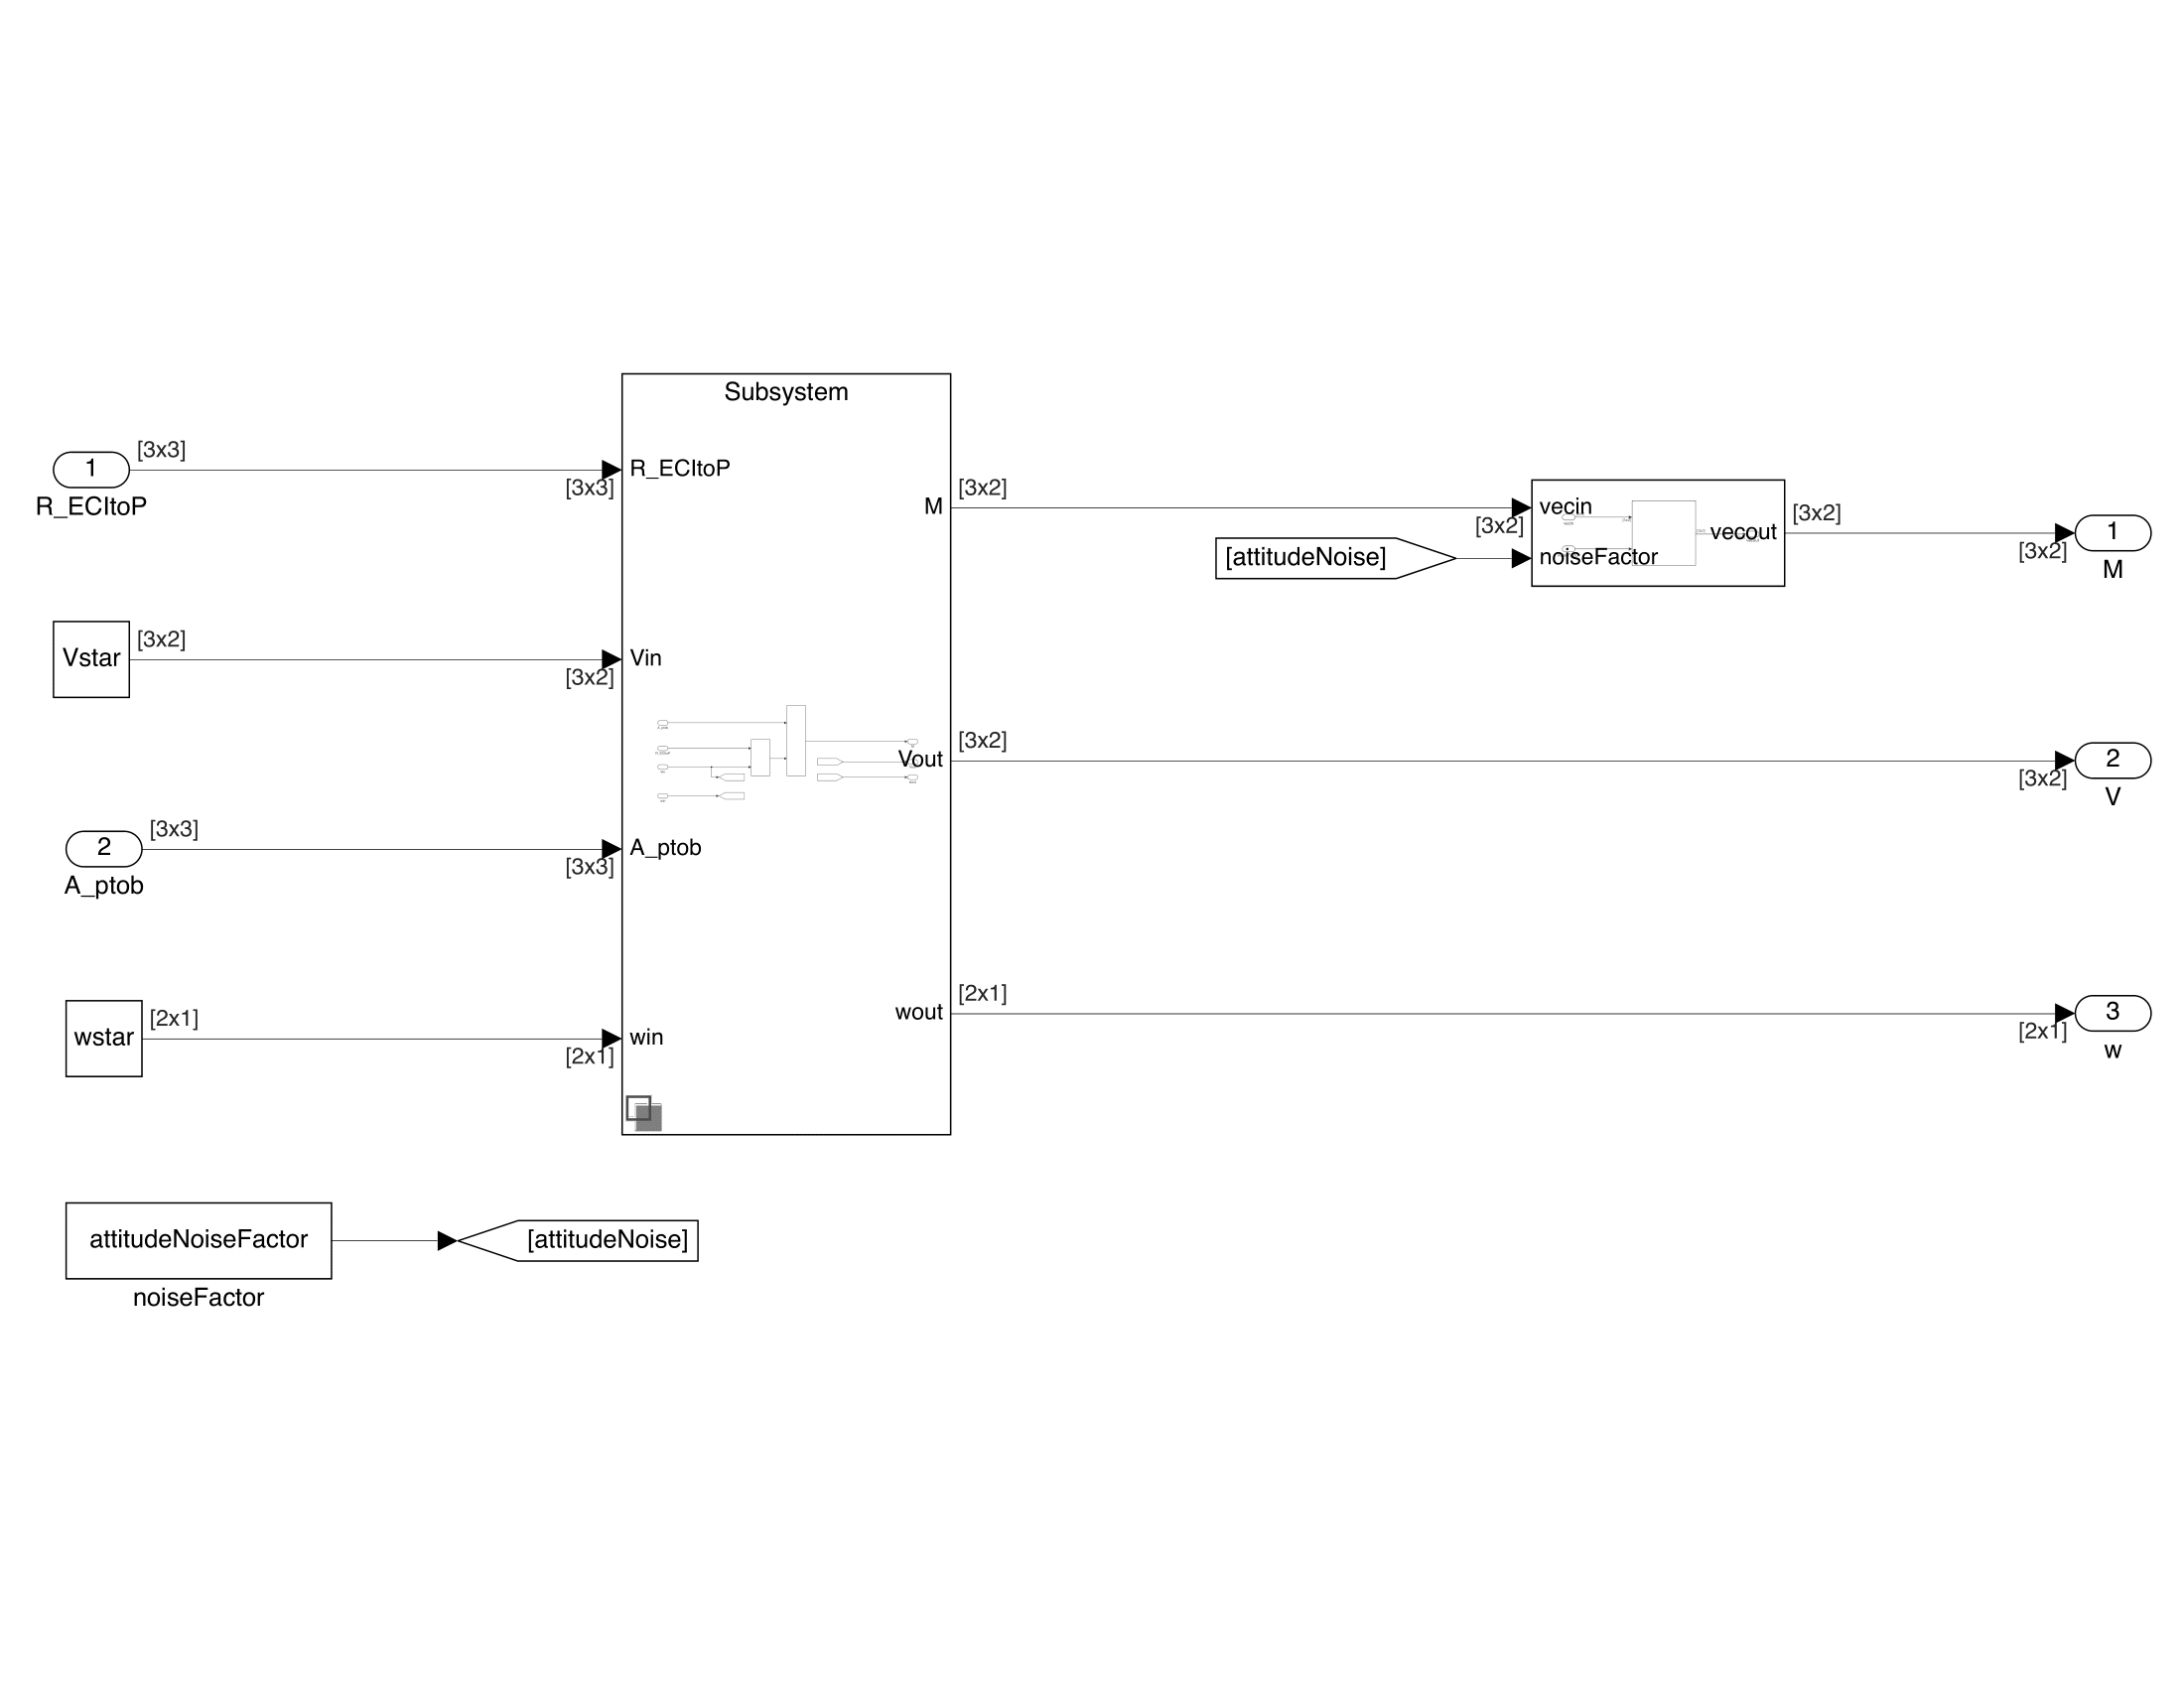
\includegraphics[trim={0.25cm 3cm 0.25cm 3cm},clip,width = 15cm]{Images/PS6/raw_meas_star.png}
    \caption{Model for Star Tracker Measurement Generation}
    \label{fig:star_tracker_meas}
\end{figure}

The model used to rotate the ground truth vectors into the body frame is seen in Figure \ref{fig:ground_truth_to_meas}.

\begin{figure}[H]
    \centering
    \captionsetup{ justification = centering }
    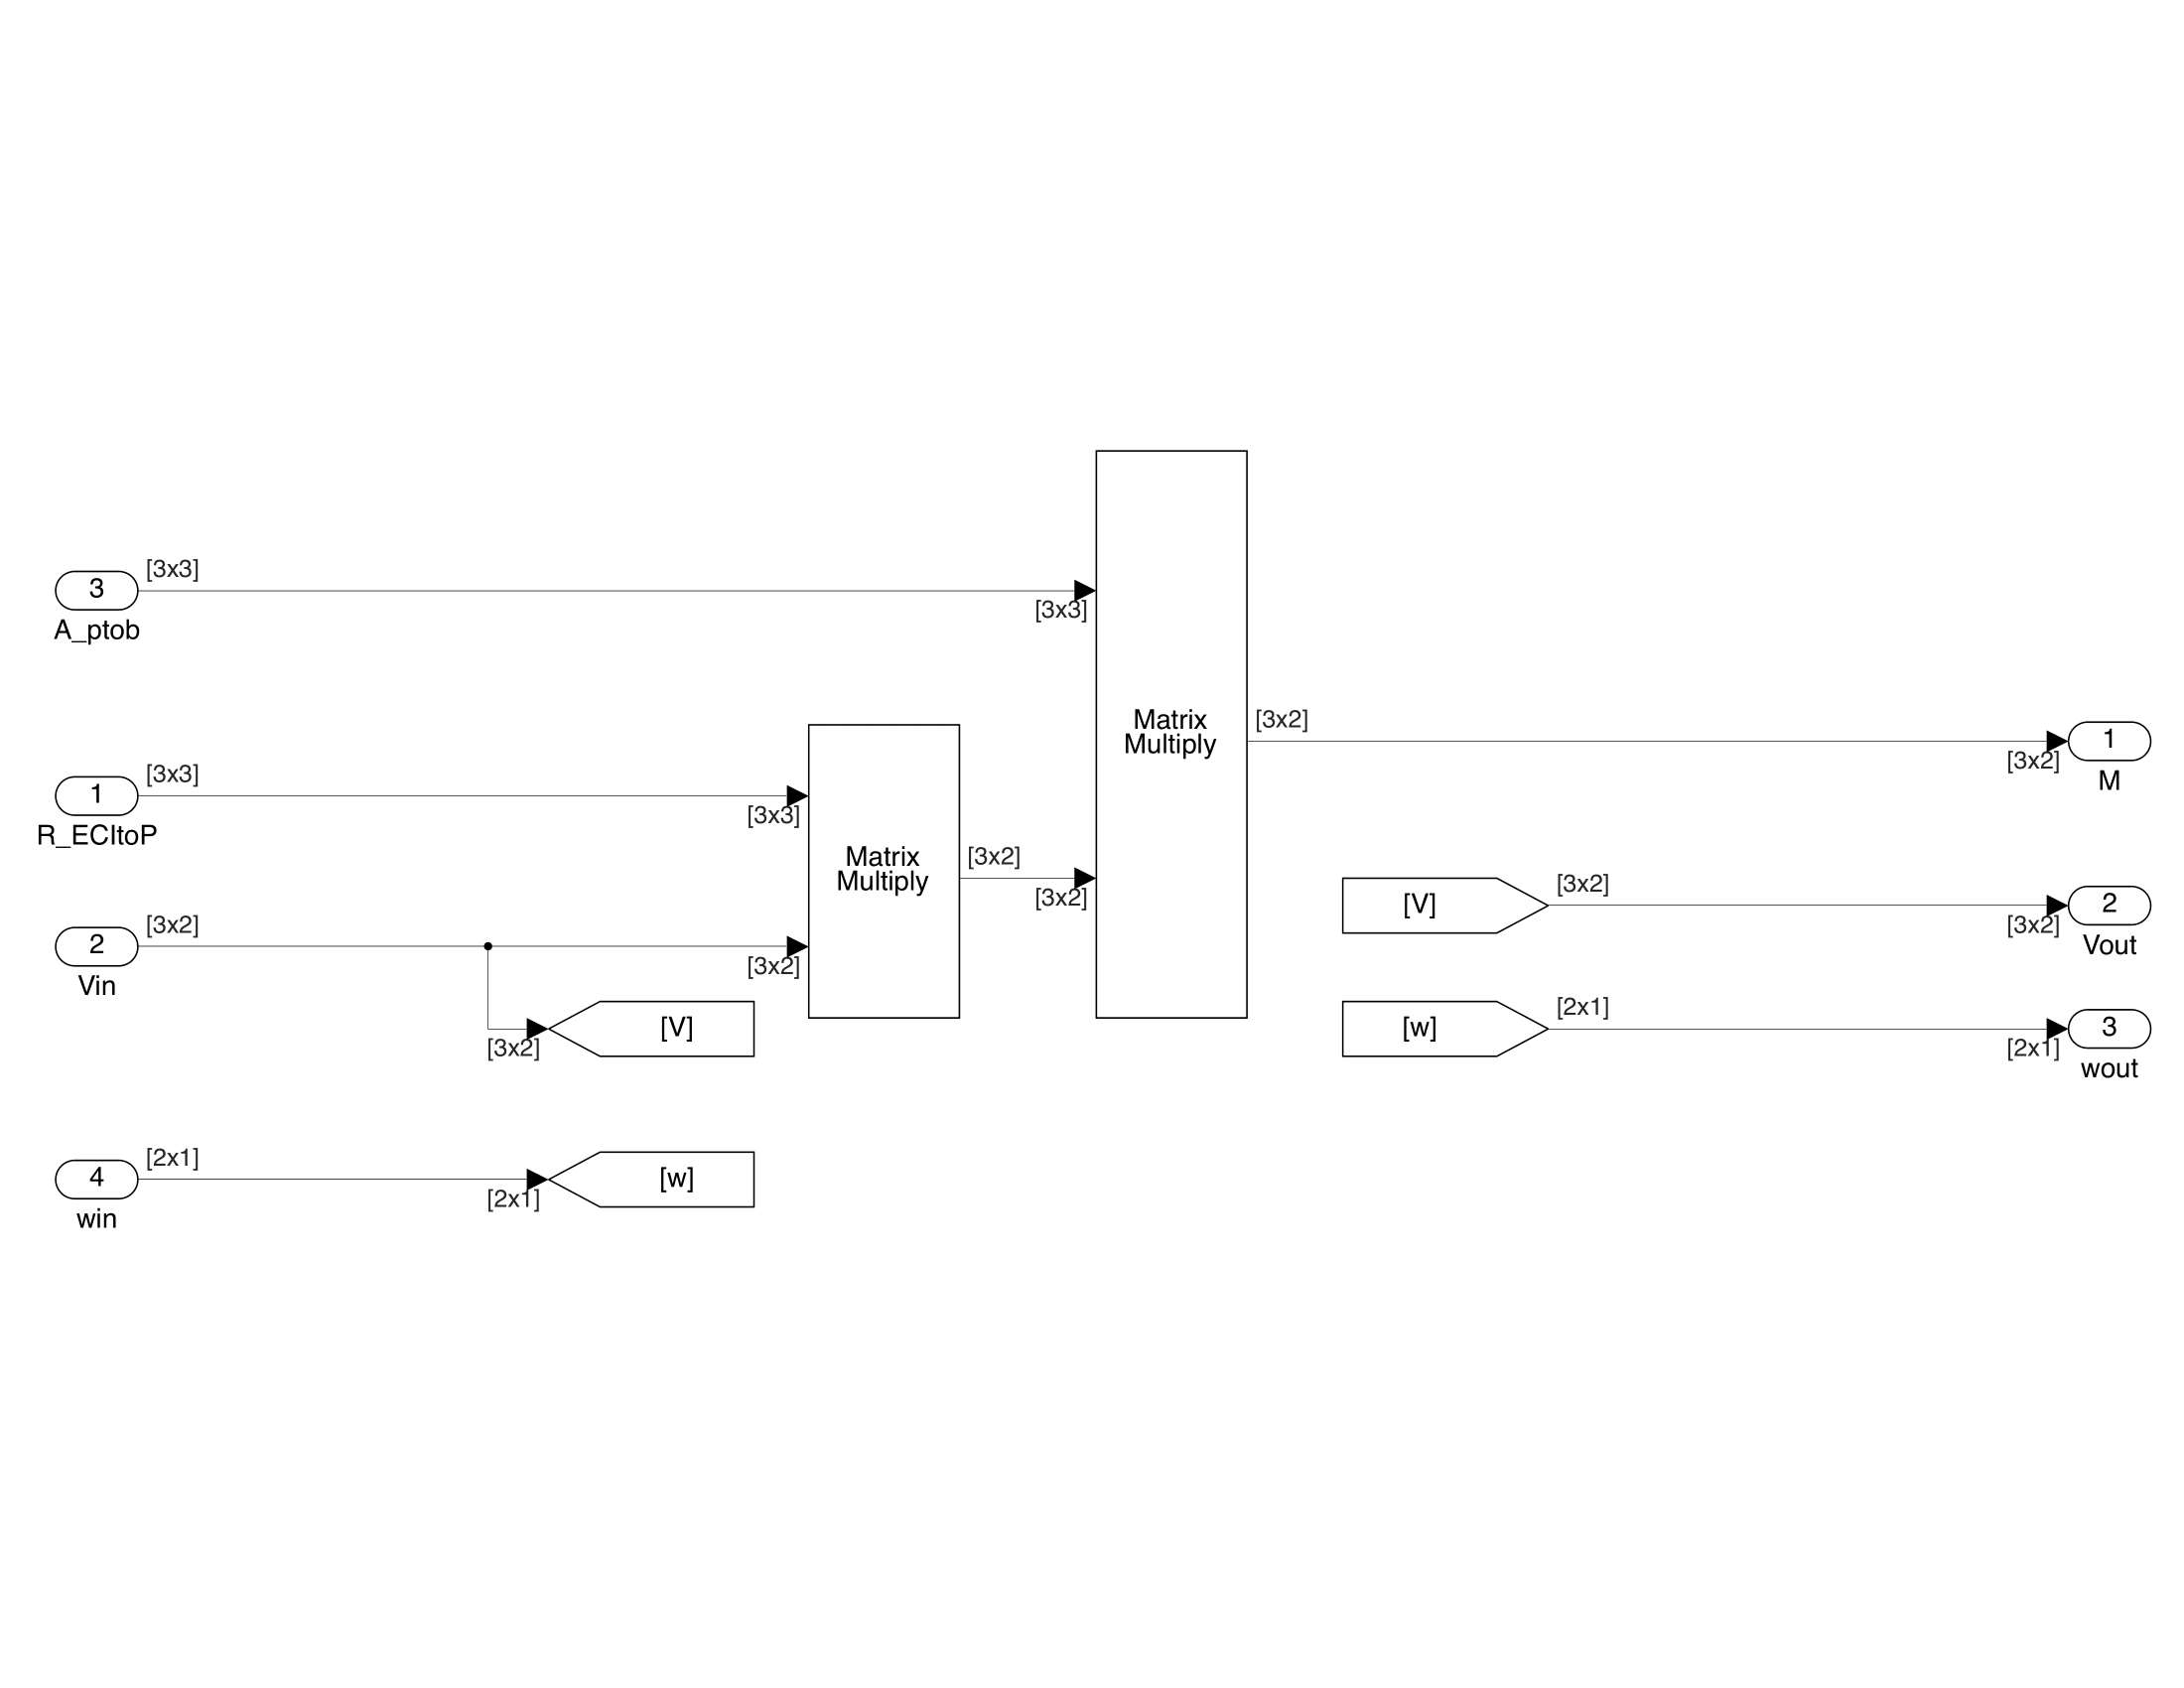
\includegraphics[trim={0.25cm 3cm 0.25cm 3cm},clip,width = 15cm]{Images/PS6/ground_truth_to_meas.png}
    \caption{Ground Truth to Measurement Model}
    \label{fig:ground_truth_to_meas}
\end{figure}

For future work, a catalog of stars would be used. Along with this, the star tracker direction in the body frame would be determined. From this, the stars that lie in the star trackers field of view would be used for the measurements while the others would be unused. This would involve allowing variable port sizes in Simulink which would pose an additional challenge.

In addition to the initialization of measurements, a system was created that would feed through sets of measurements that contain 3 or more vectors, but will create a triad if only two measurements are available. Additionally, for the case where only two measurements are available, the errors can be mitigated by creating two fictitious measurements first before generating the triad that ultimately gets fed into the deterministic determination algorithm. The feed through model can be seen in Figure \ref{fig:feedthrough_meas} whereas the fictitious measurement model can be seen in Figure \ref{fig:fictitious_meas}.

\begin{figure}[H]
    \centering
    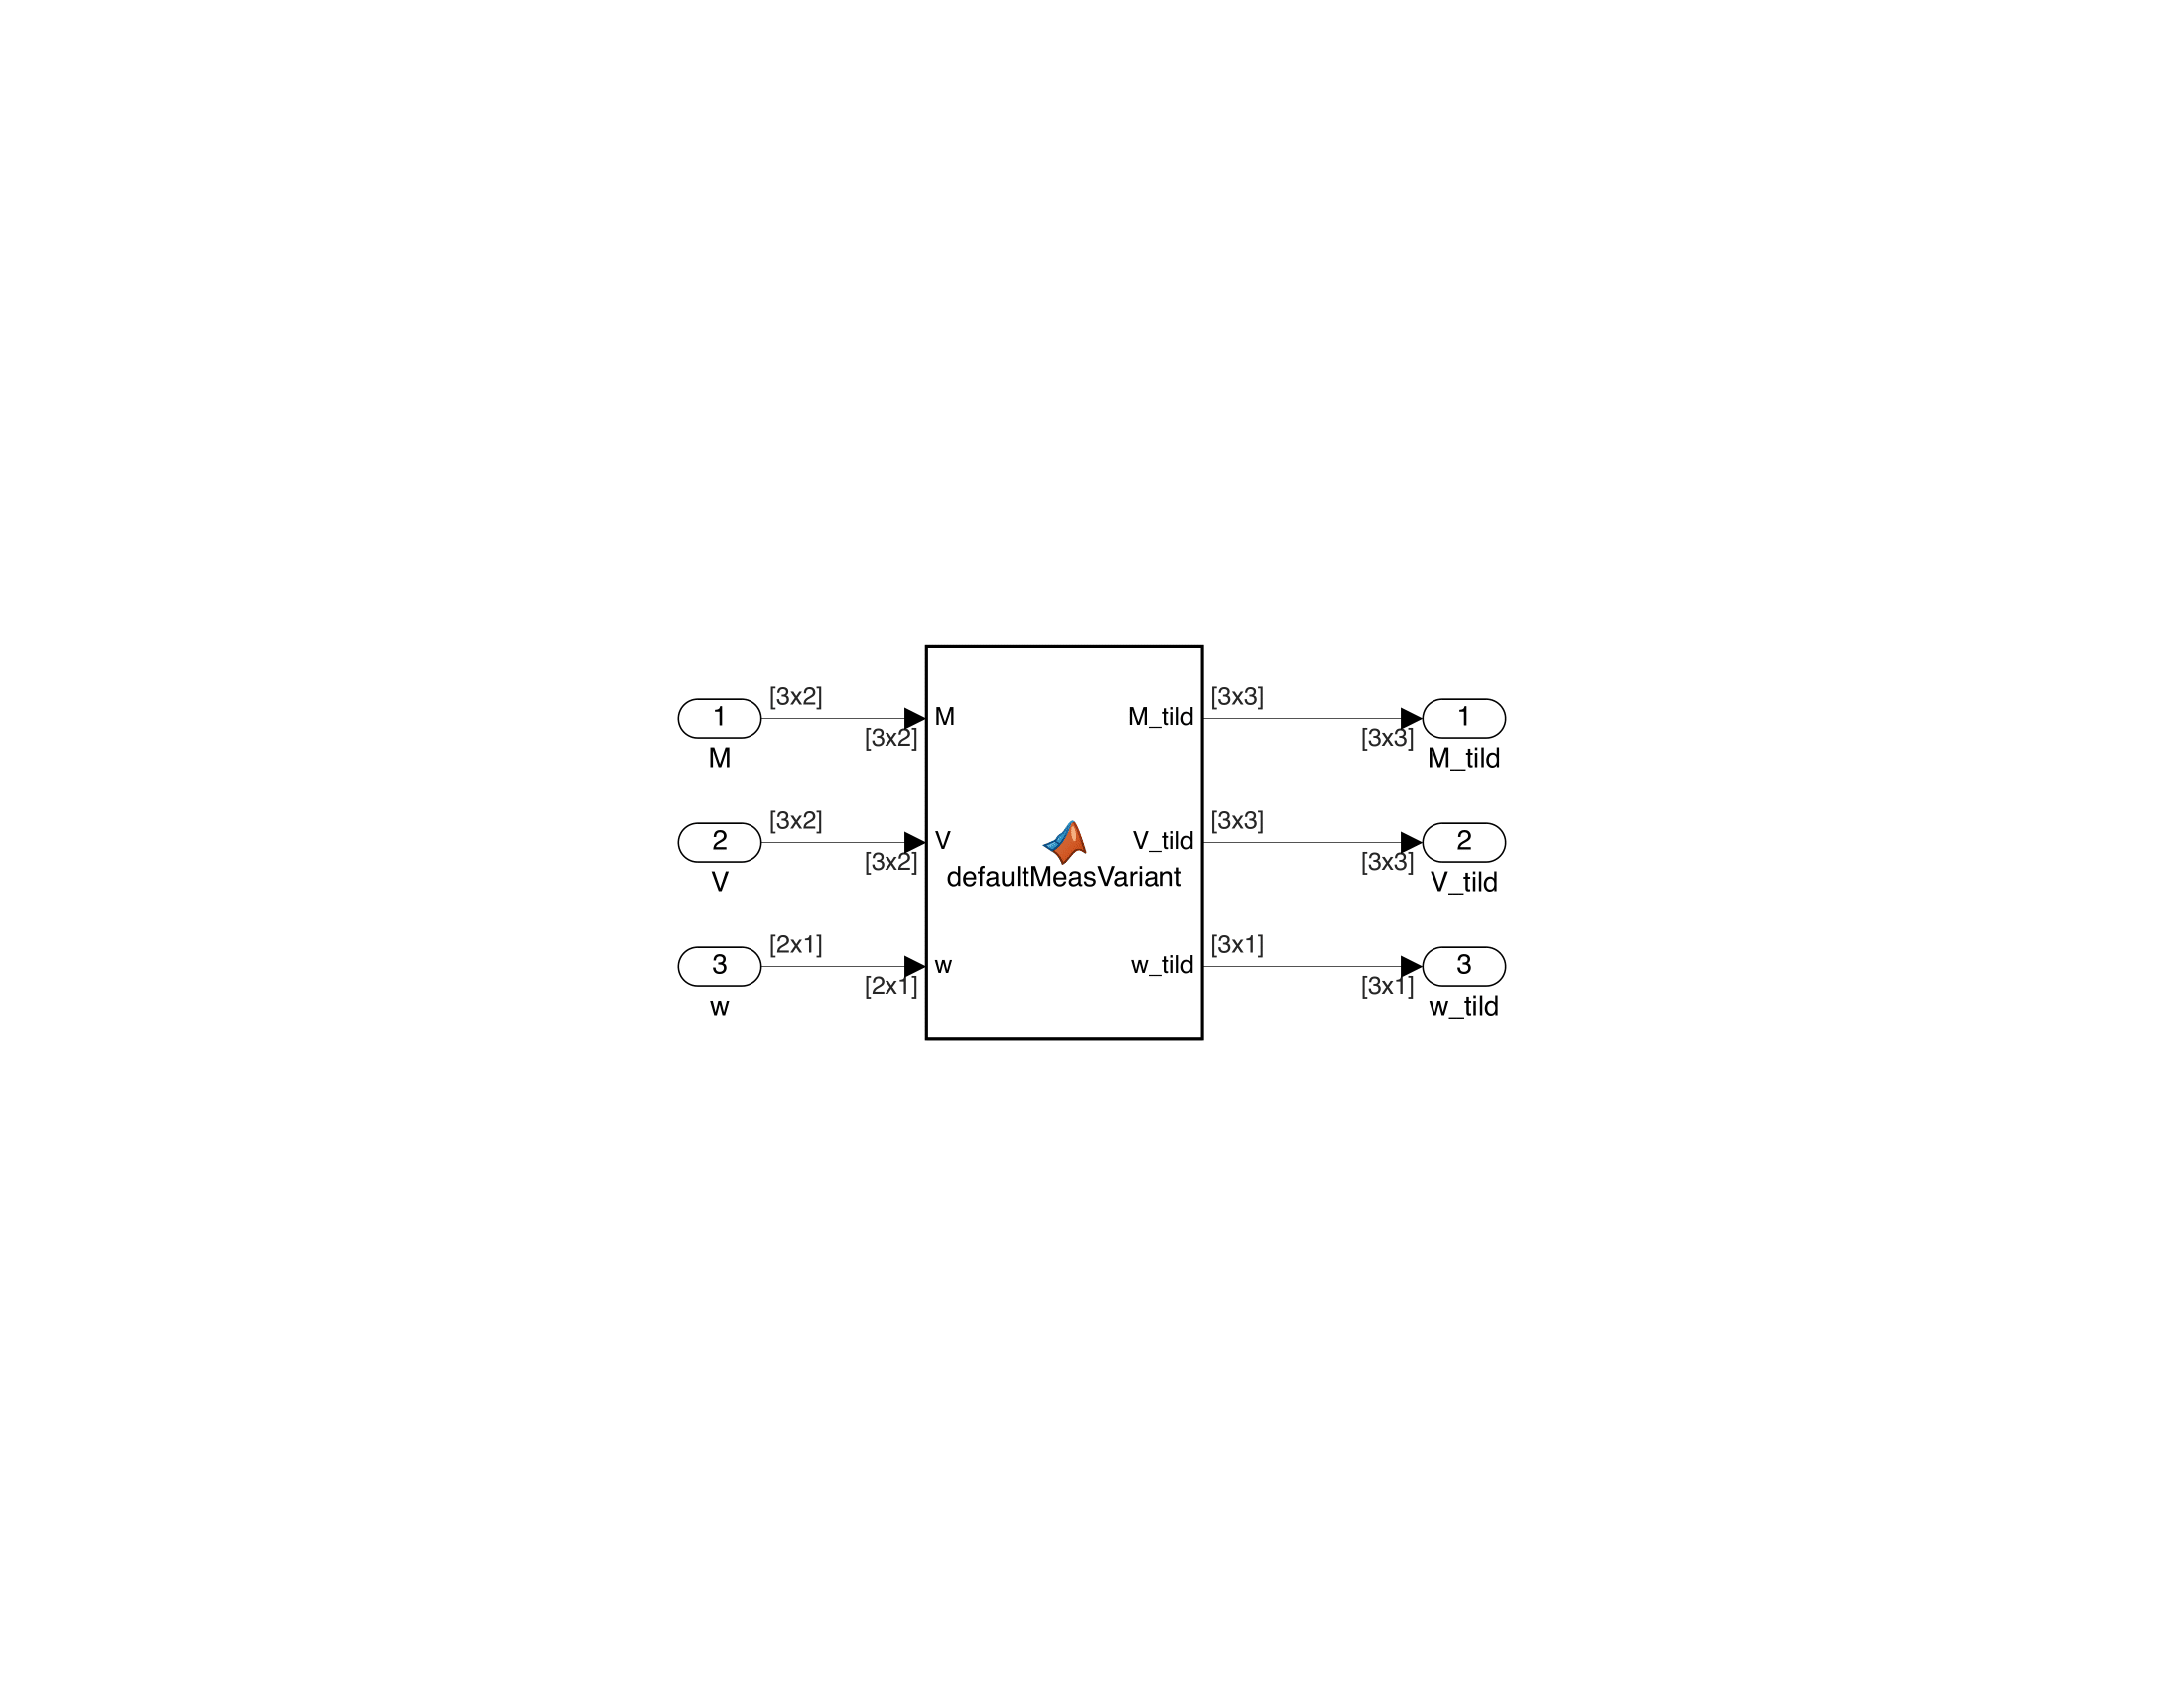
\includegraphics[trim={8cm 5cm 8cm 7cm},clip,width = 12cm]{Images/PS6/feedthrough_meas.png}
\end{figure}

\begin{figure}[H]
    \centering
    \captionsetup{ justification = centering }
    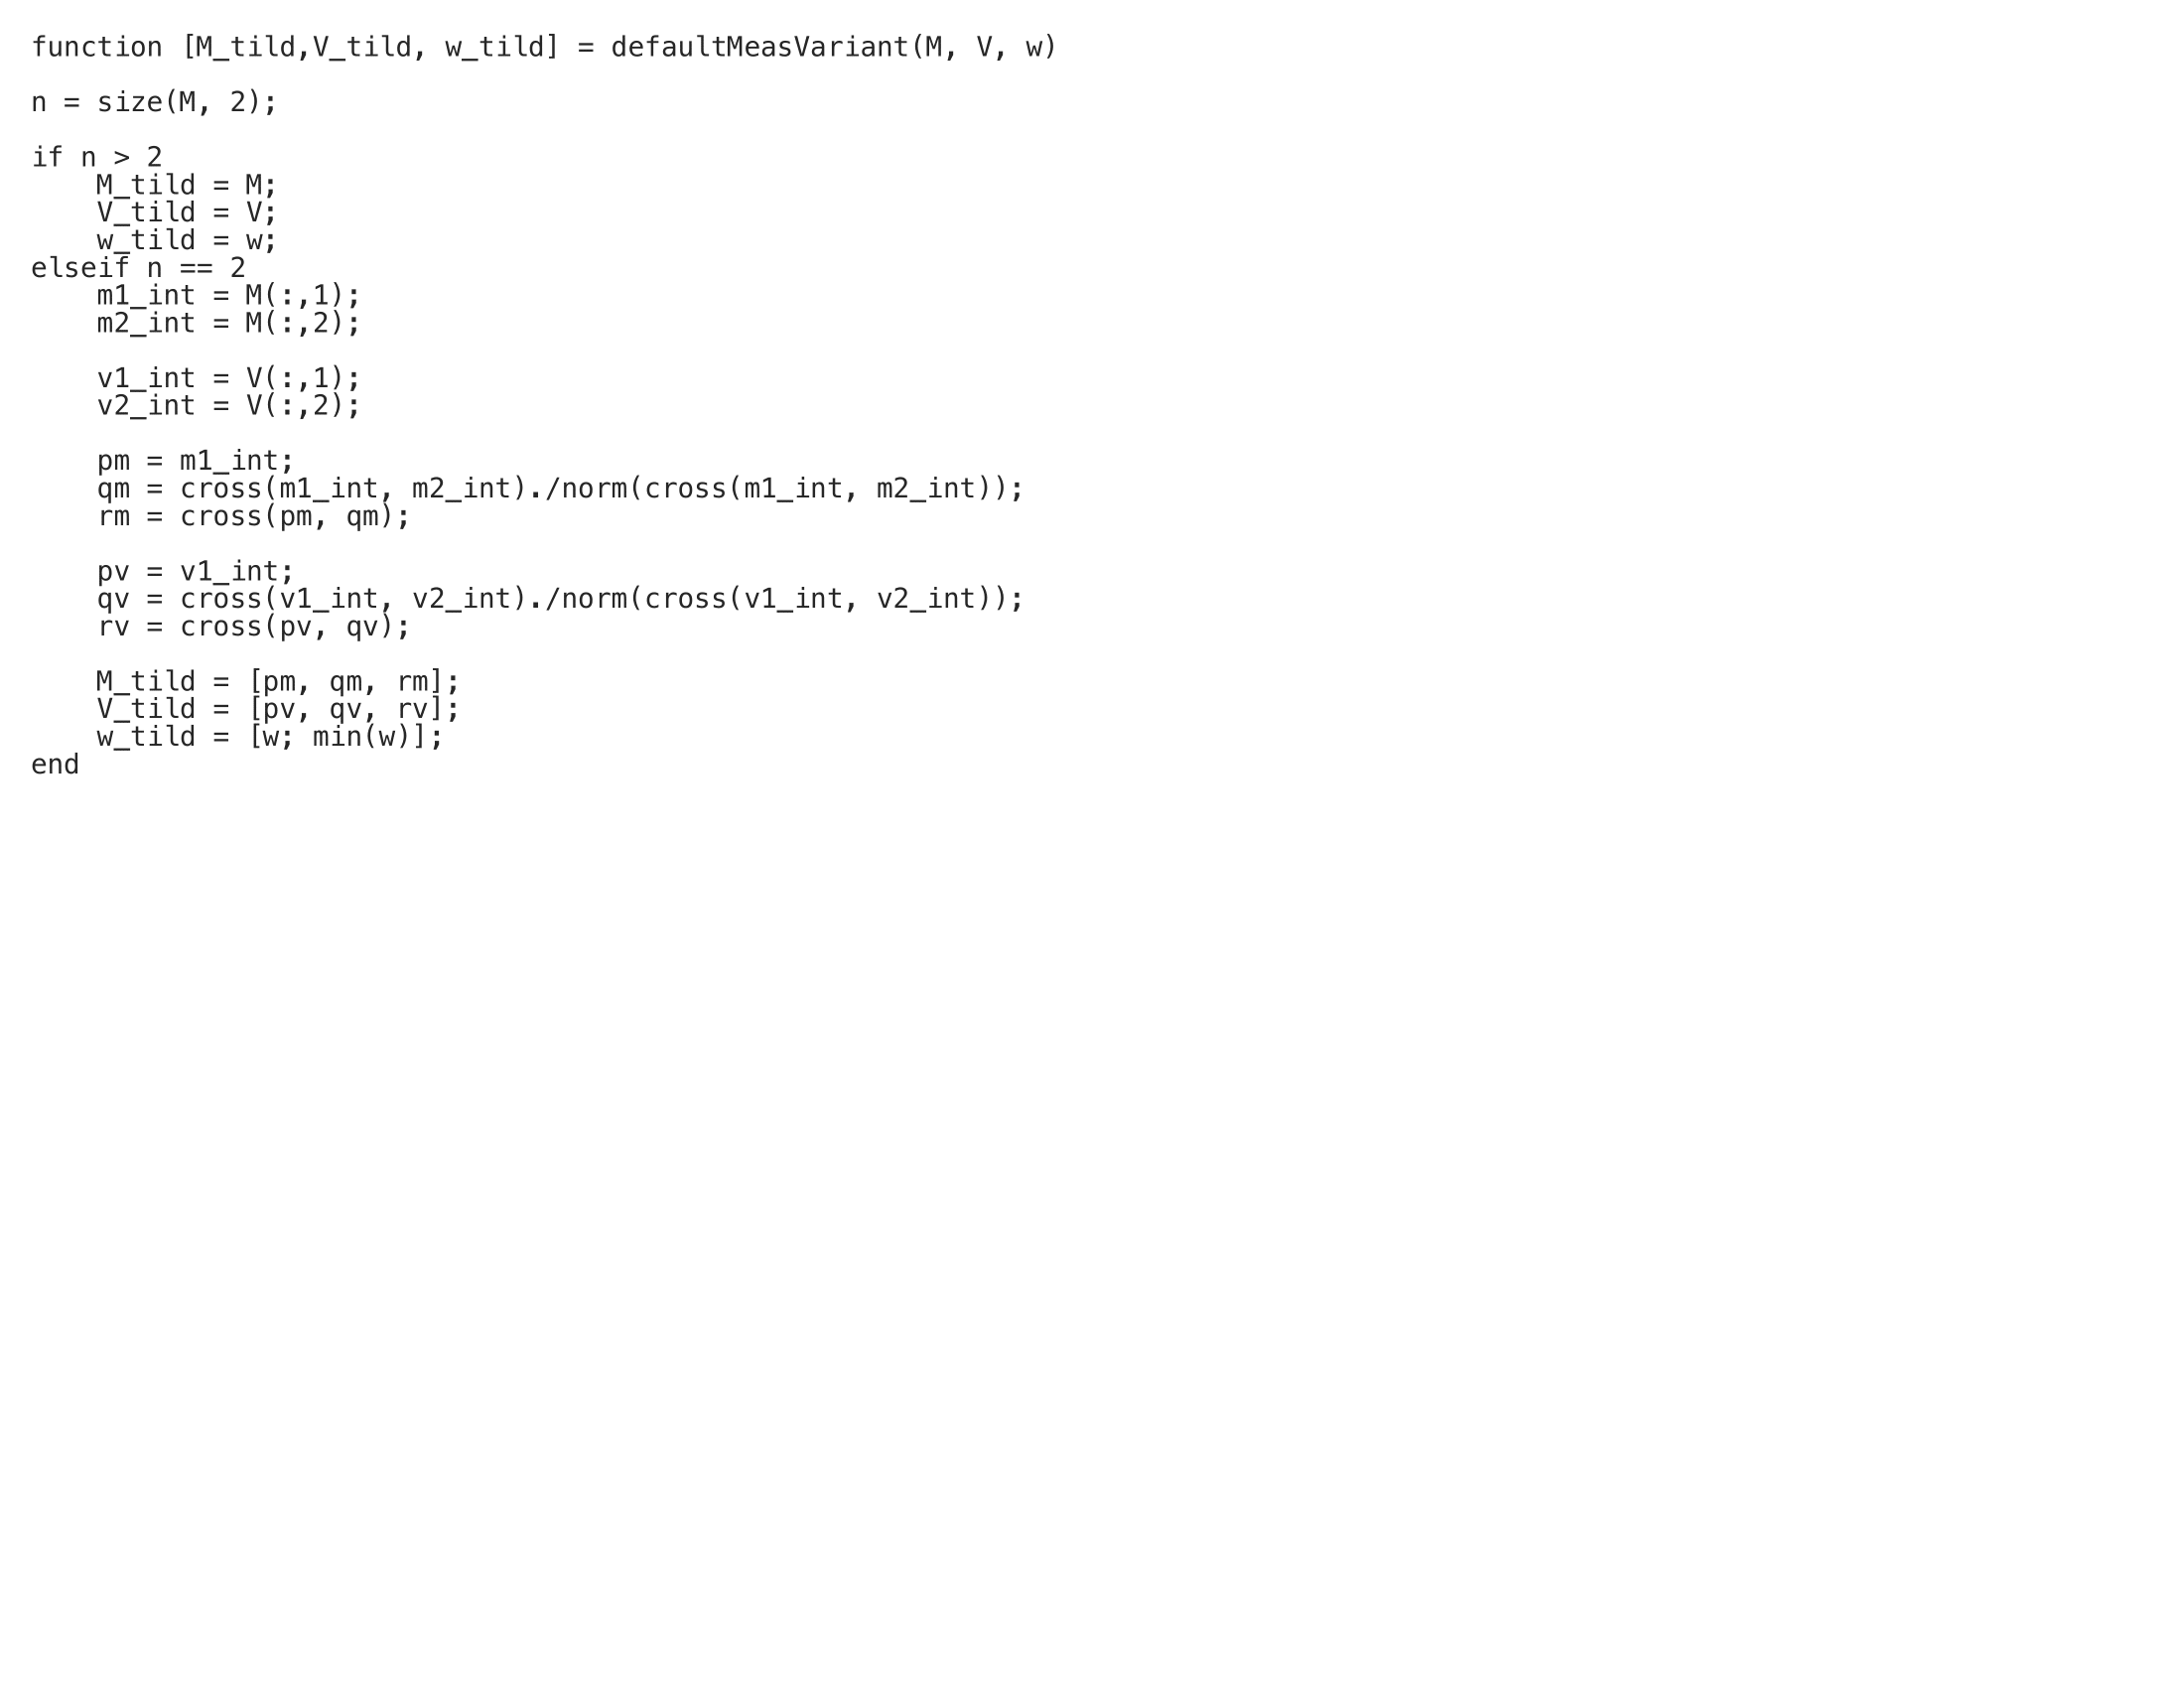
\includegraphics[trim={0cm 10cm 10cm 0cm},clip,width = 15cm]{Images/PS6/feedthrough_meas_code.png}
    \caption{Model for Star Tracker Measurement Generation}
    \label{fig:feedthrough_meas}
\end{figure}

\begin{figure}[H]
    \centering
    \captionsetup{ justification = centering }
    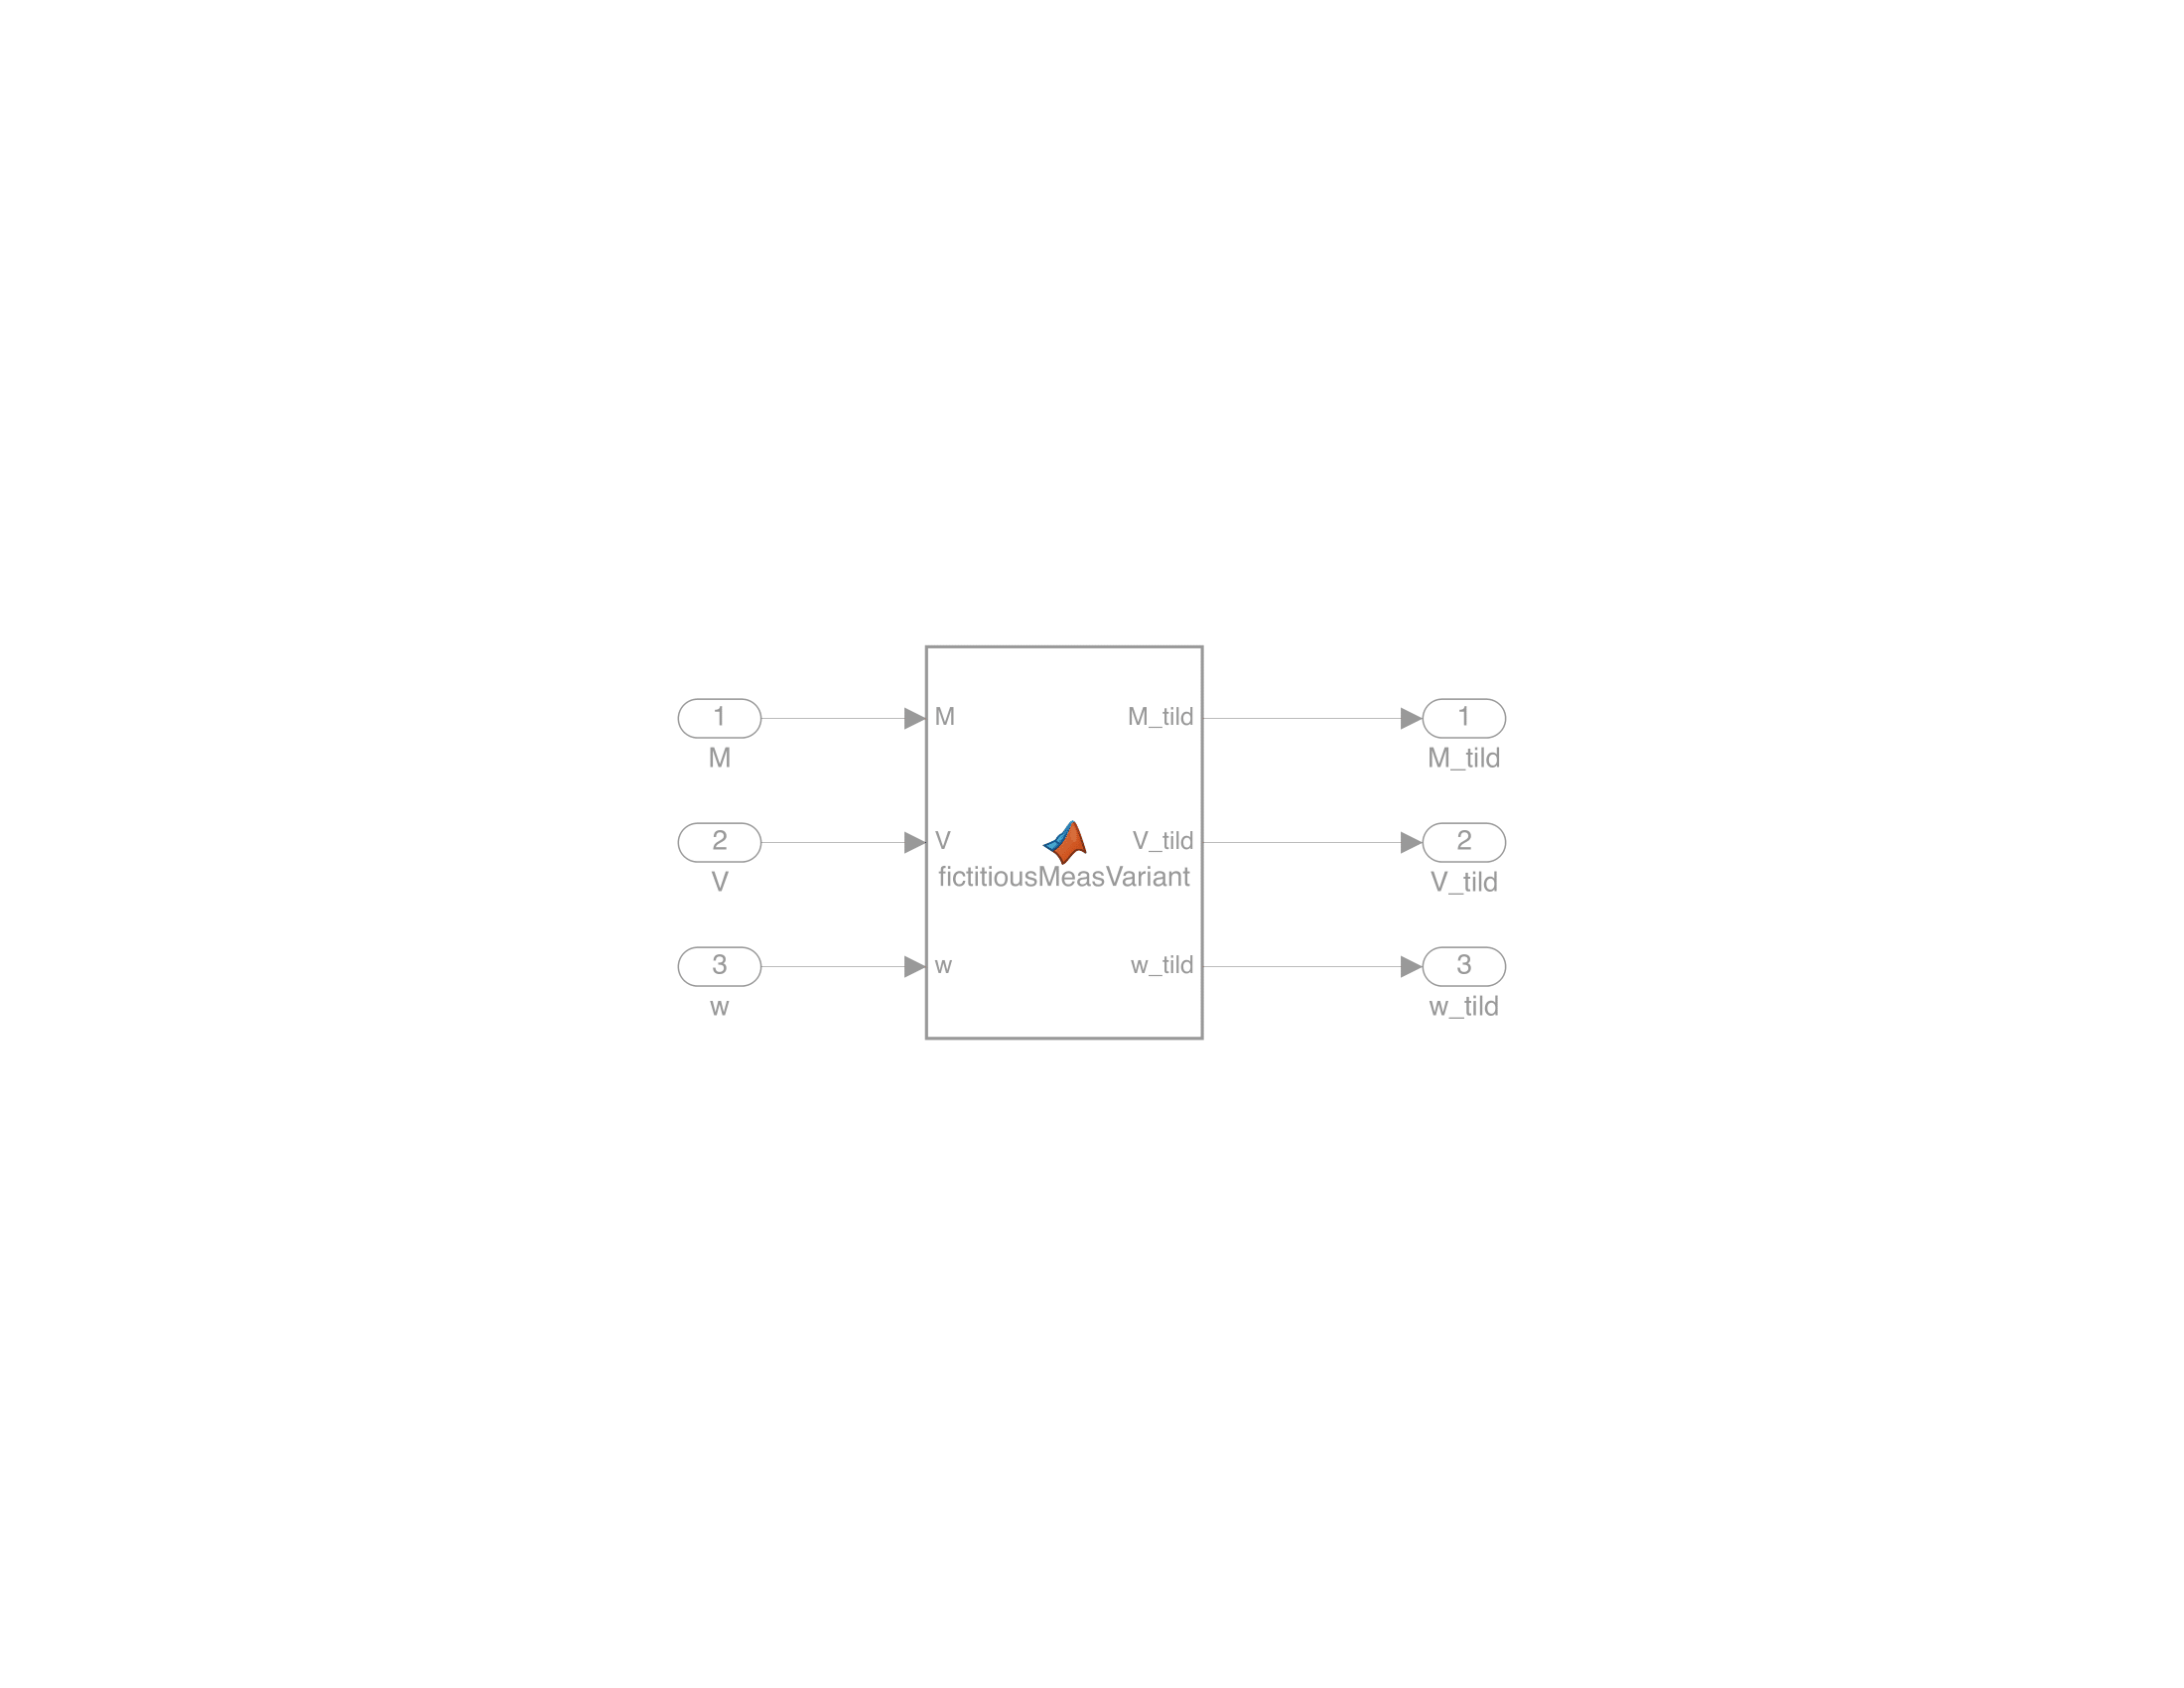
\includegraphics[trim={8cm 8cm 8cm 8cm},clip,width = 12cm]{Images/PS6/fict_meas.png}
\end{figure}

\begin{figure}[H]
    \centering
    \captionsetup{ justification = centering }
    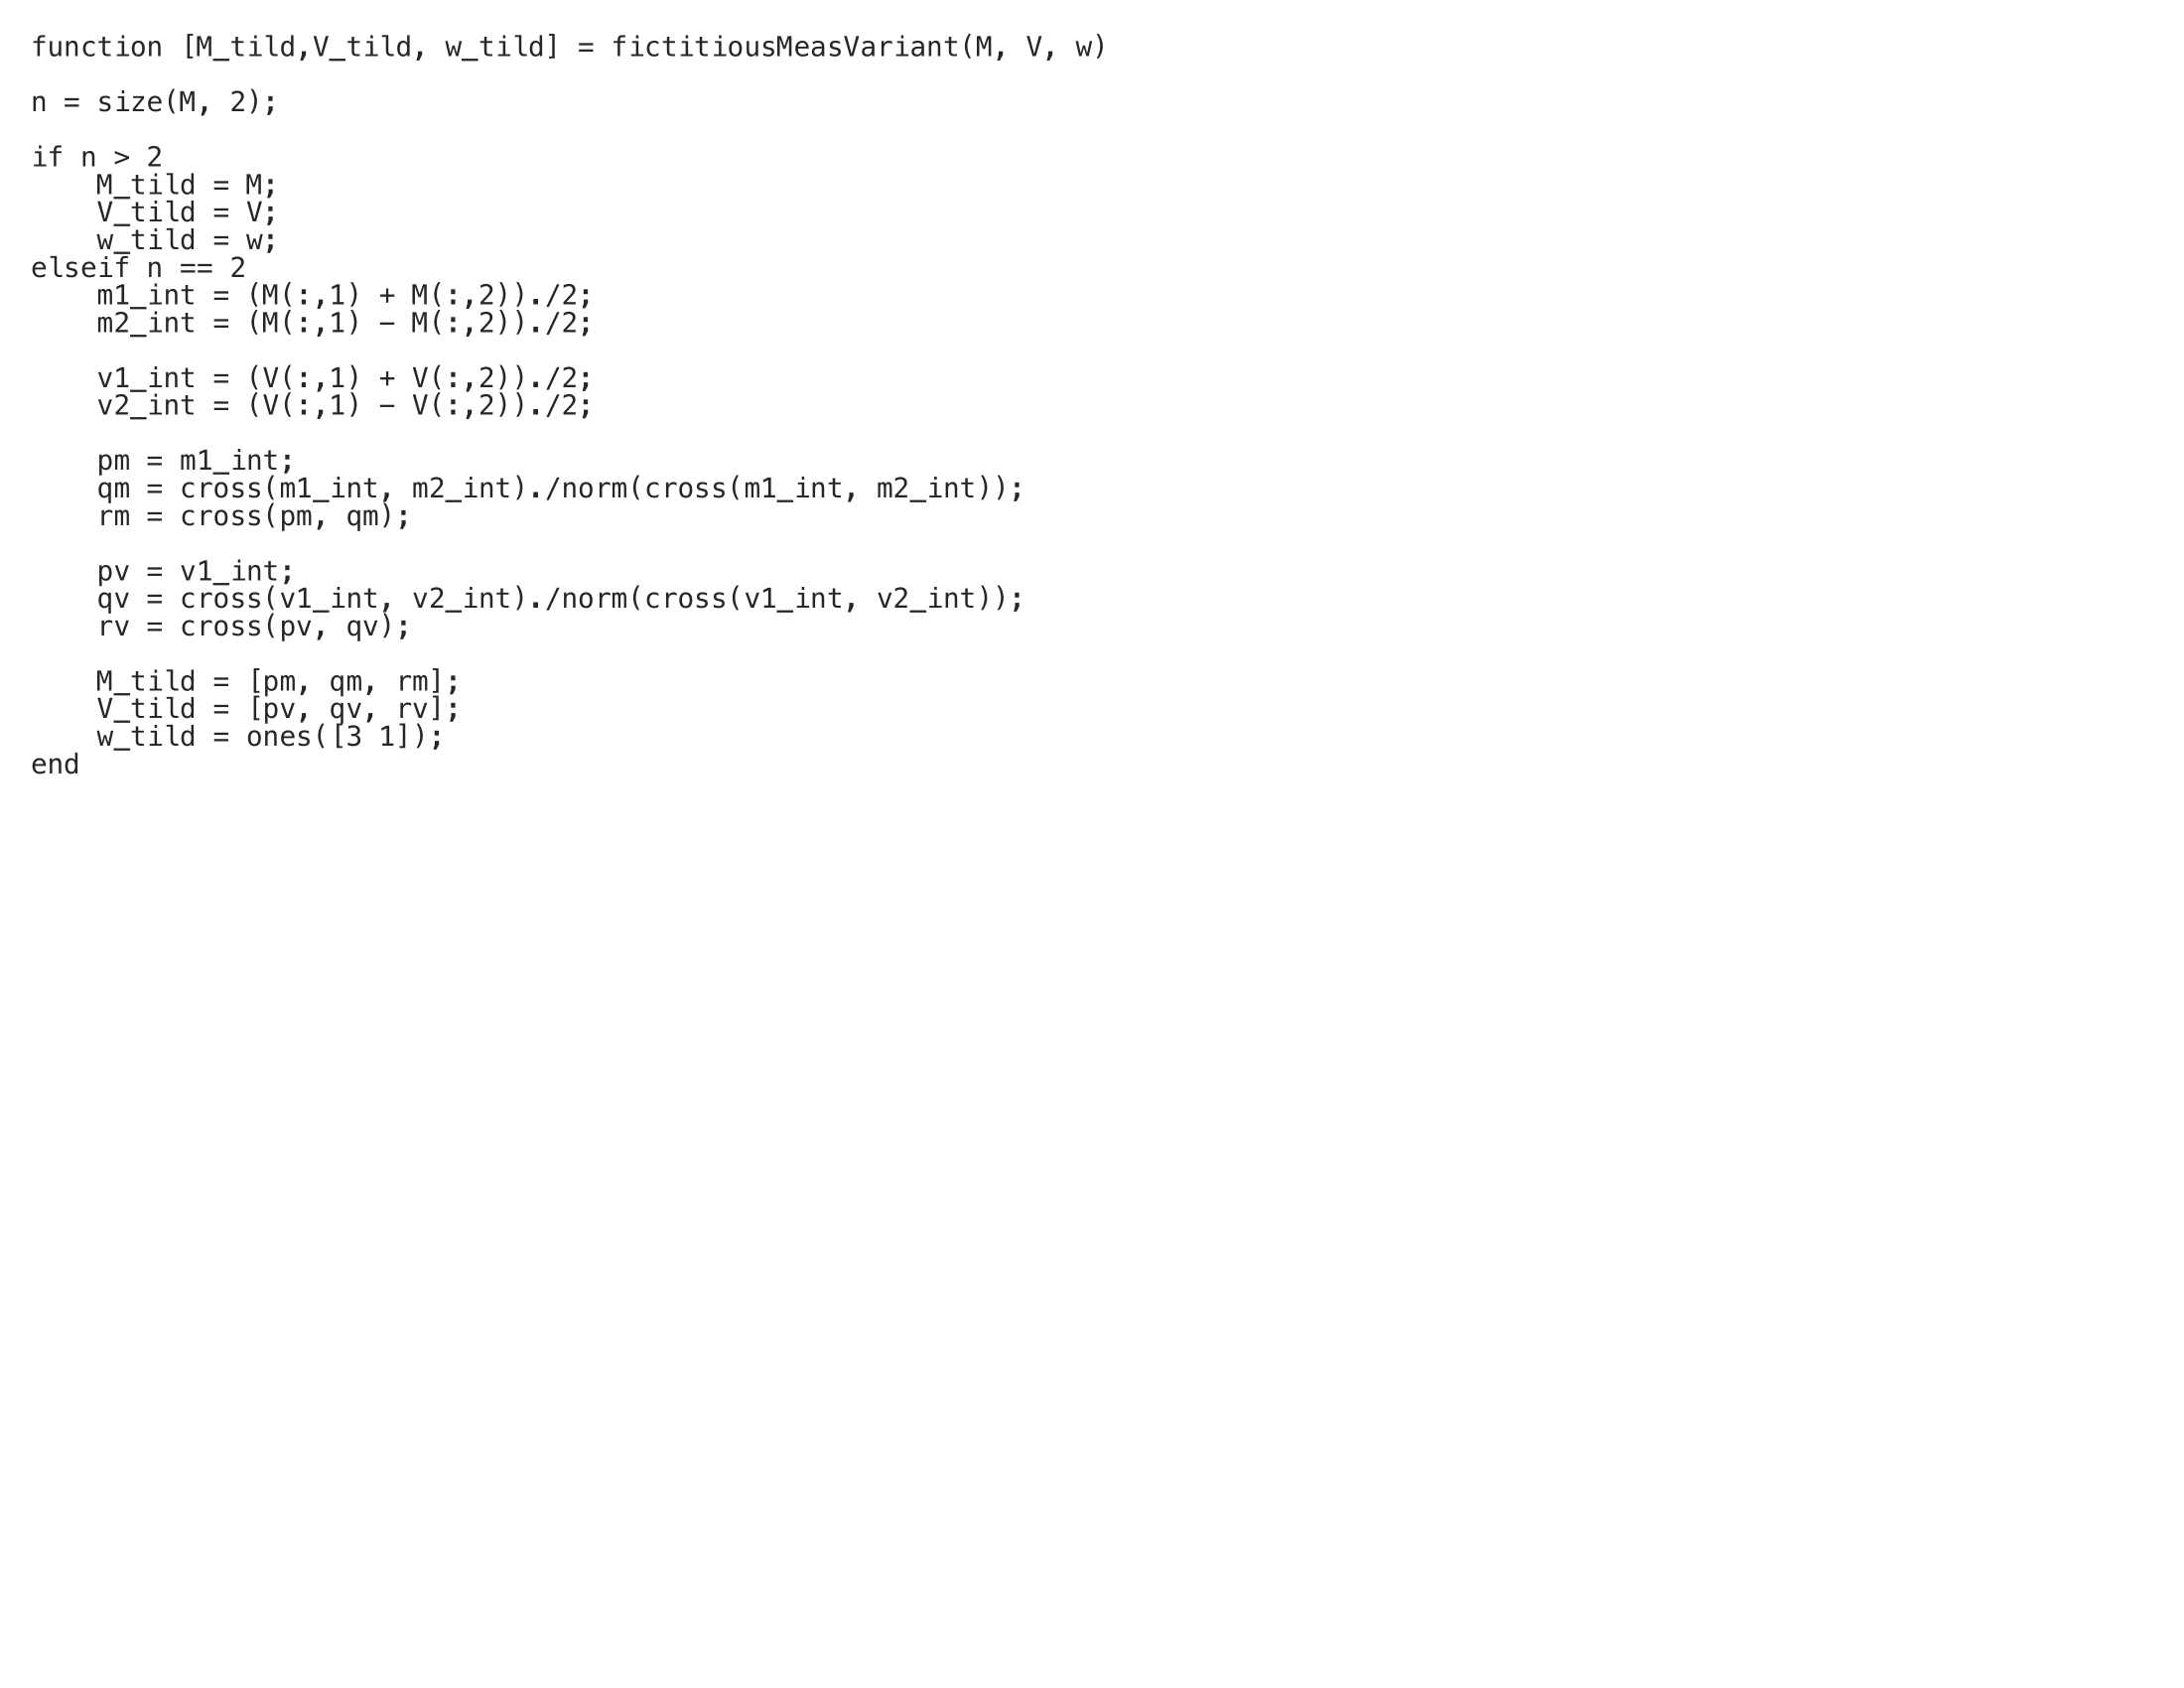
\includegraphics[trim={0cm 10cm 10cm 0cm},clip,width = 15cm]{Images/PS6/fict_meas_code.png}
    \caption{Model for Star Tracker Measurement Generation}
    \label{fig:fictitious_meas}
\end{figure}

\subsection{Problem 5 - Assume a certain set of sensors. In general, a number of unit = vectors and angular velocities can be considered as measurements.}

\subsubsection{Implement the deterministic attitude determination algorithm discussed in class and its variant which uses fictitious measurements to spread the errors across the measurements}

The deterministic attitude determination method was implemented using the model shown in Figure \ref{fig:det_attitude}.

\begin{figure}[H]
    \centering
    \captionsetup{ justification = centering }
    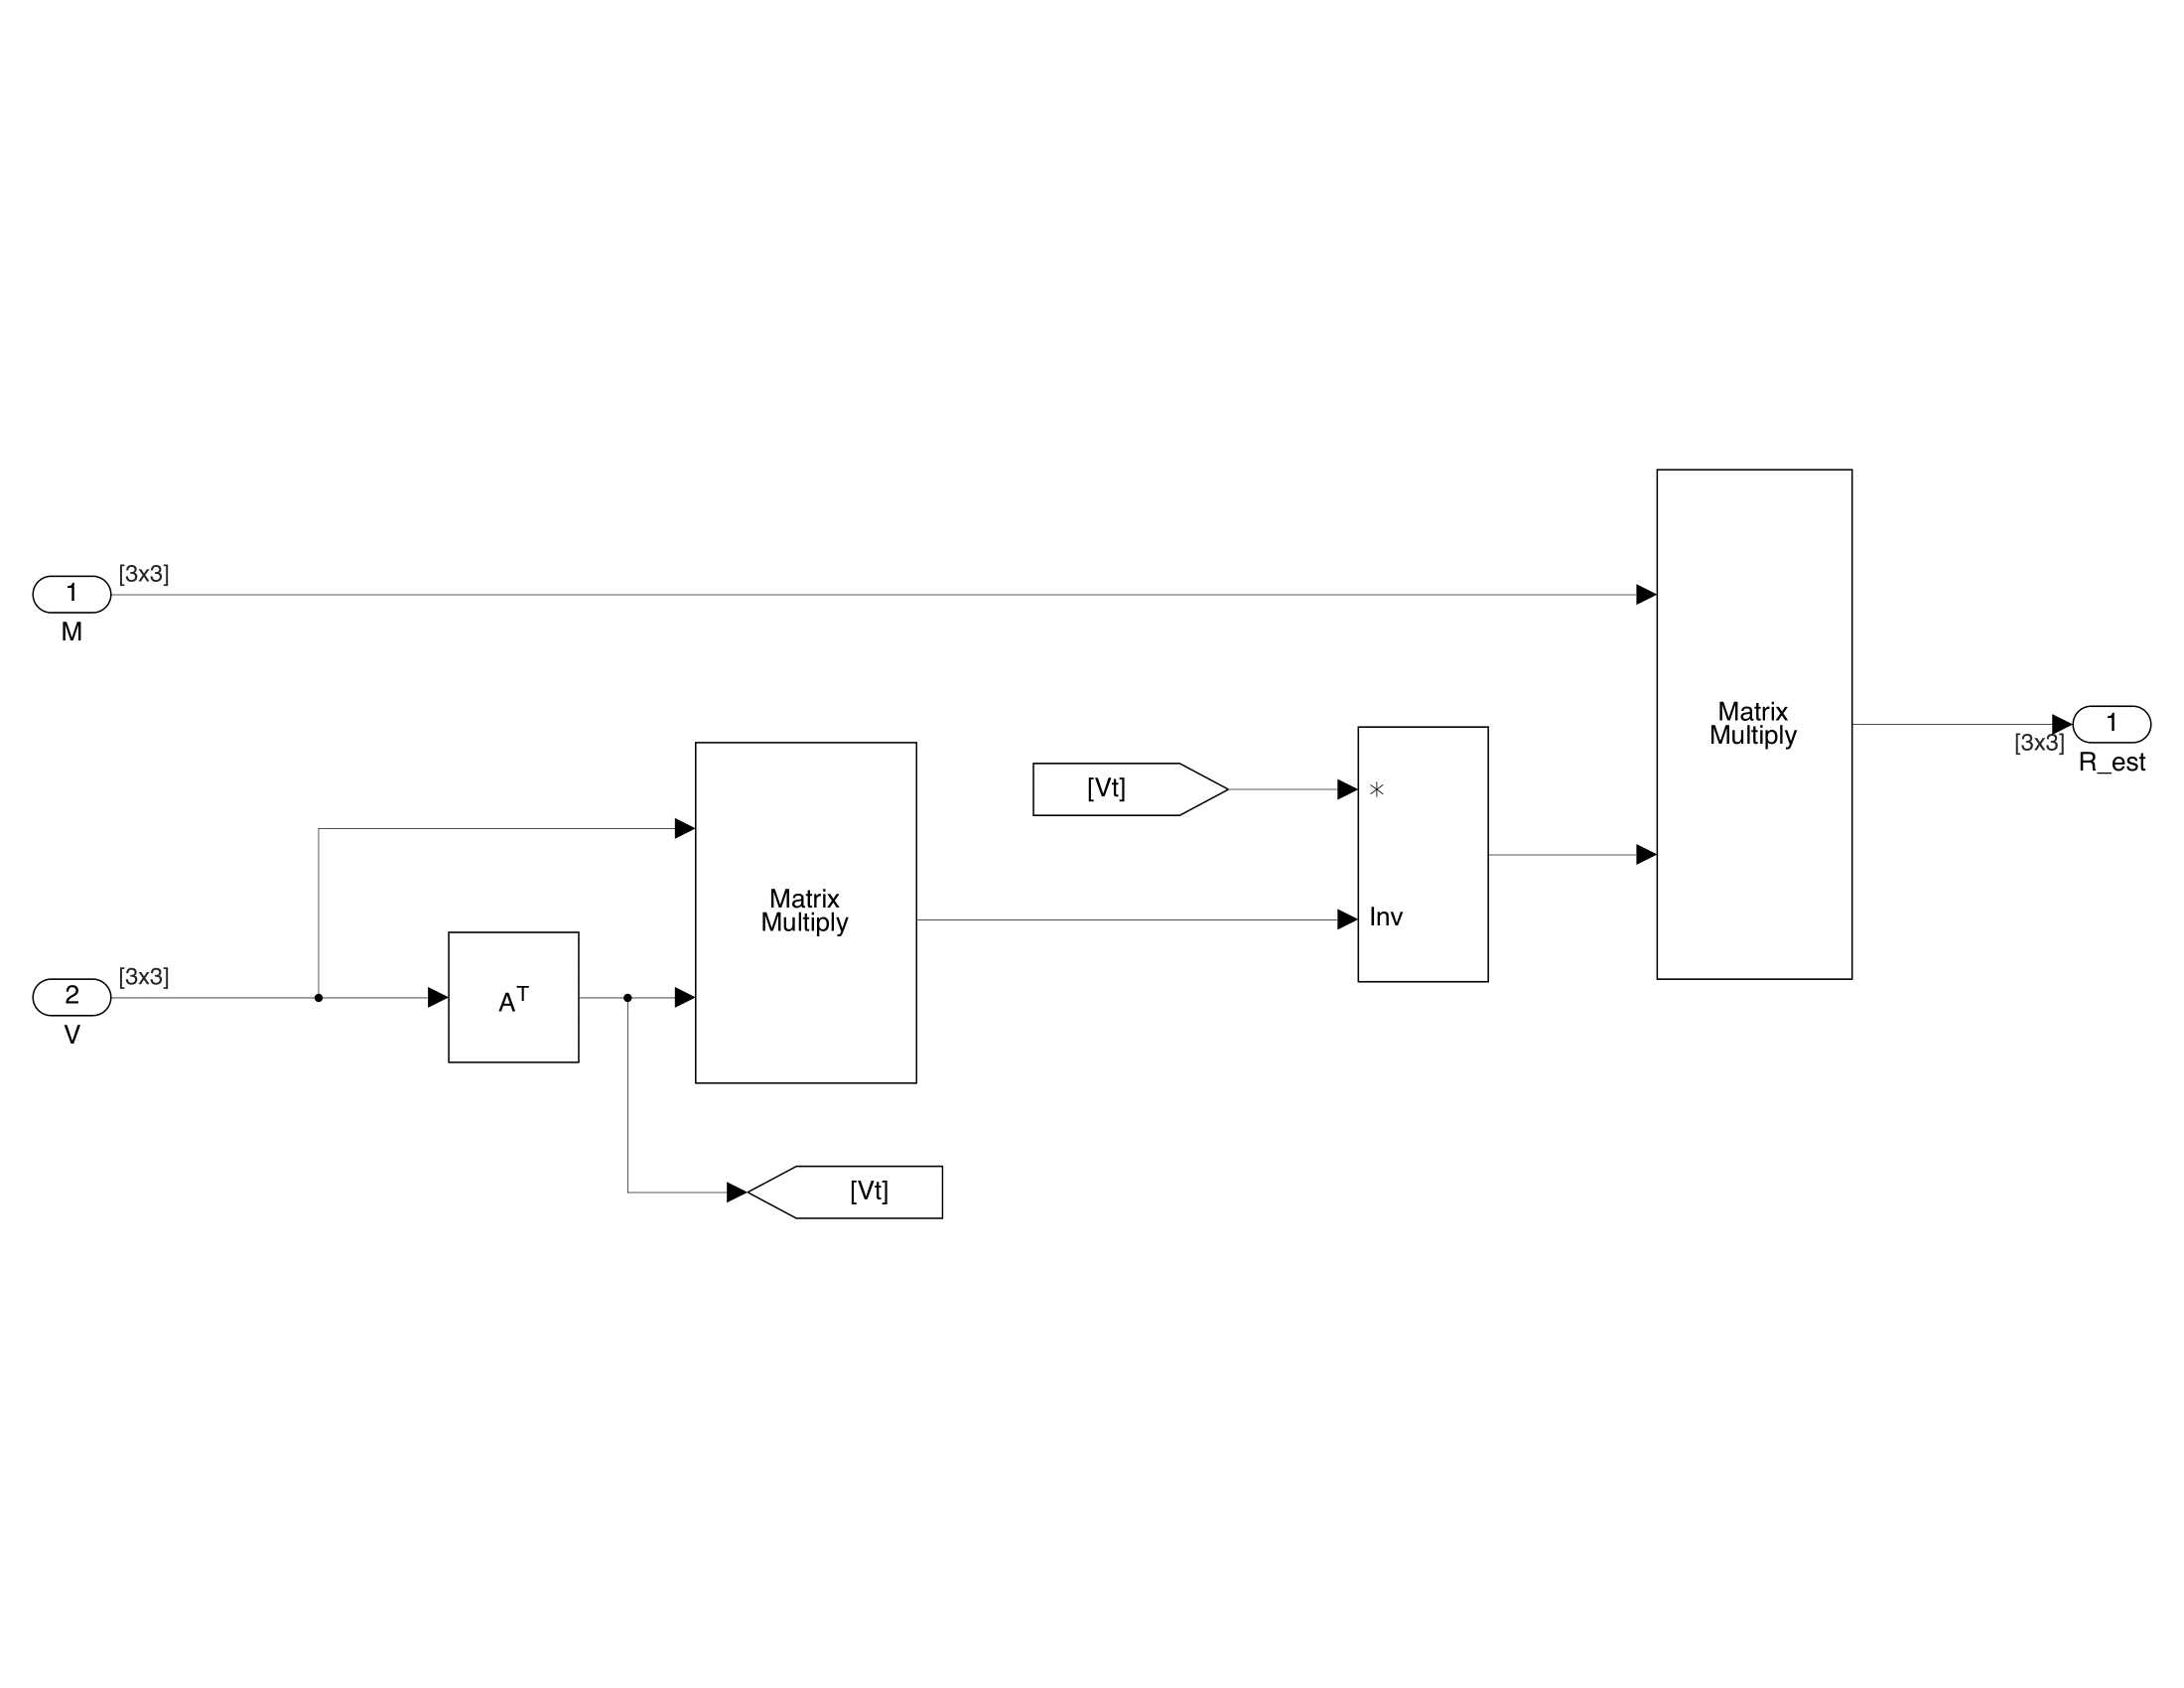
\includegraphics[trim={0.25cm 3cm 0.25cm 5cm},clip,width = 15cm]{Images/PS6/deterministicAttitude-1.png}
    \caption{Deterministic Attitude Determination Model}
    \label{fig:det_attitude}
\end{figure}

\subsubsection{Implement the statistical attitude determination algorithm discussed in class (q-method)}

The statistical attitude determination method, or the so called q-method, was implemented using the model depicted in Figure \ref{fig:stat_attitude}. 

\begin{figure}[H]
    \centering
    \captionsetup{ justification = centering }
    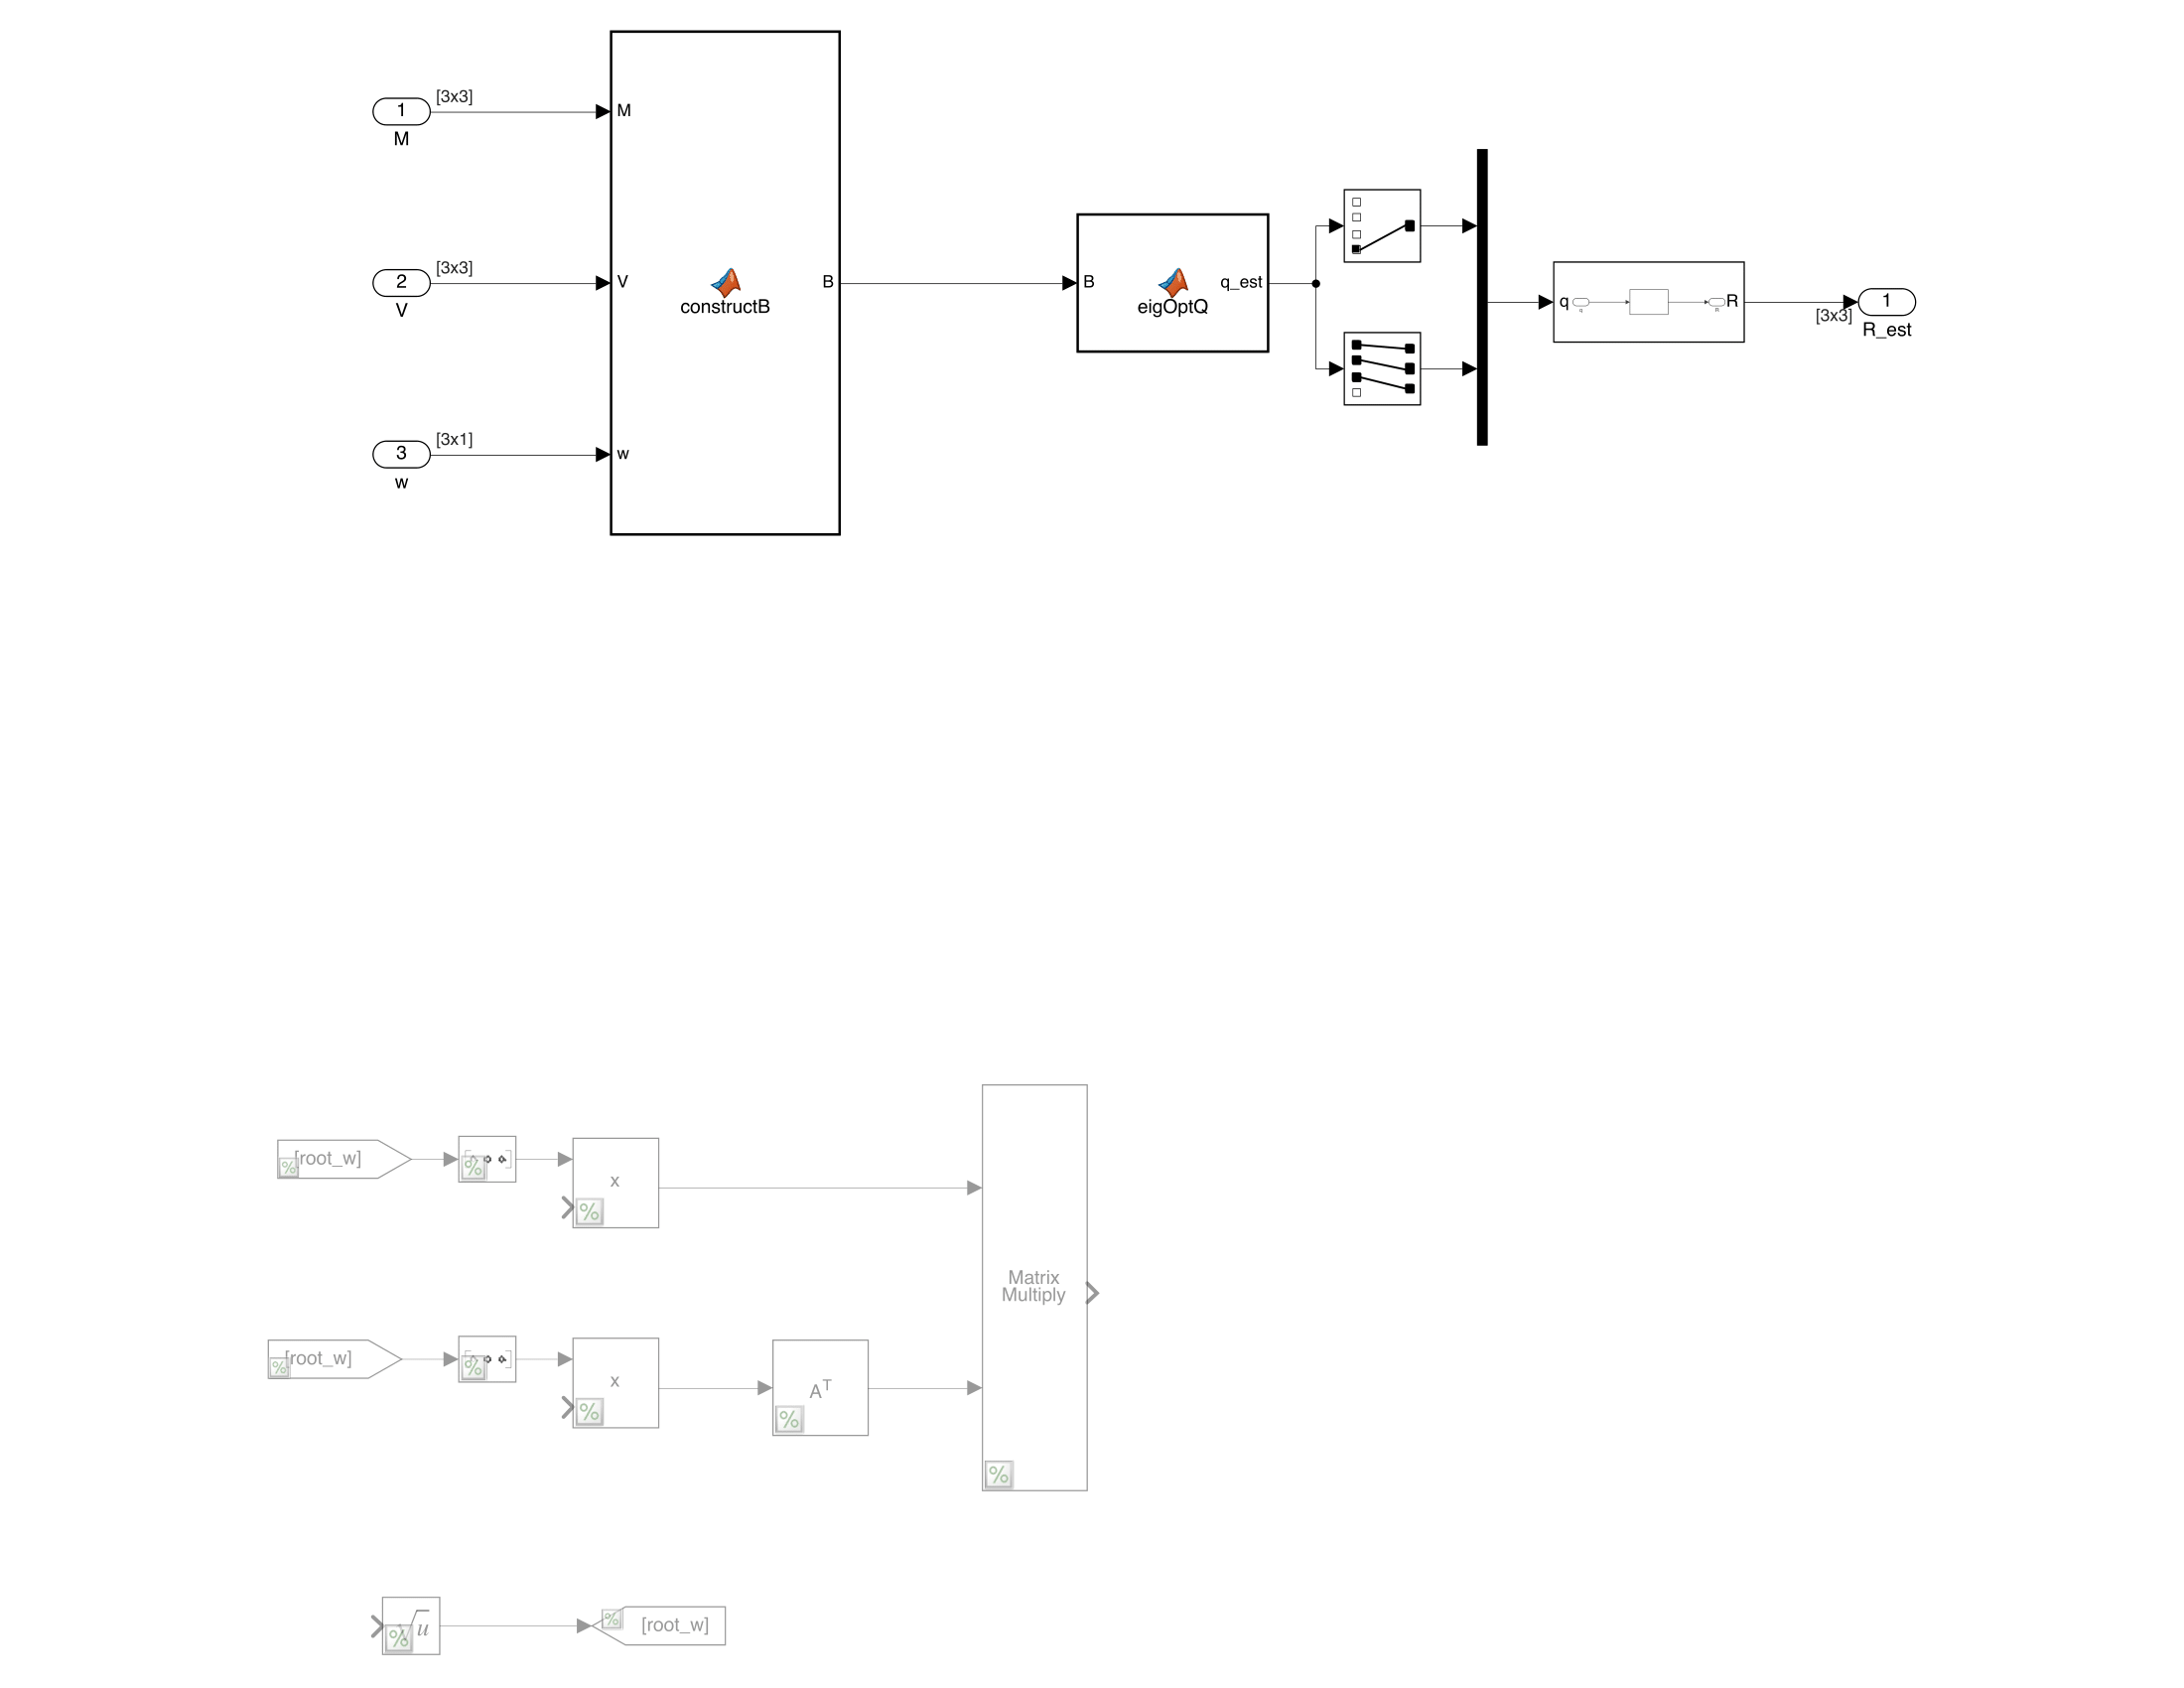
\includegraphics[trim={4cm 13cm 3cm 0cm},clip,width = 15cm]{Images/PS6/statisticalAttitude-1.png}
\end{figure}

\begin{figure}[H]
    \centering
    \captionsetup{ justification = centering }
    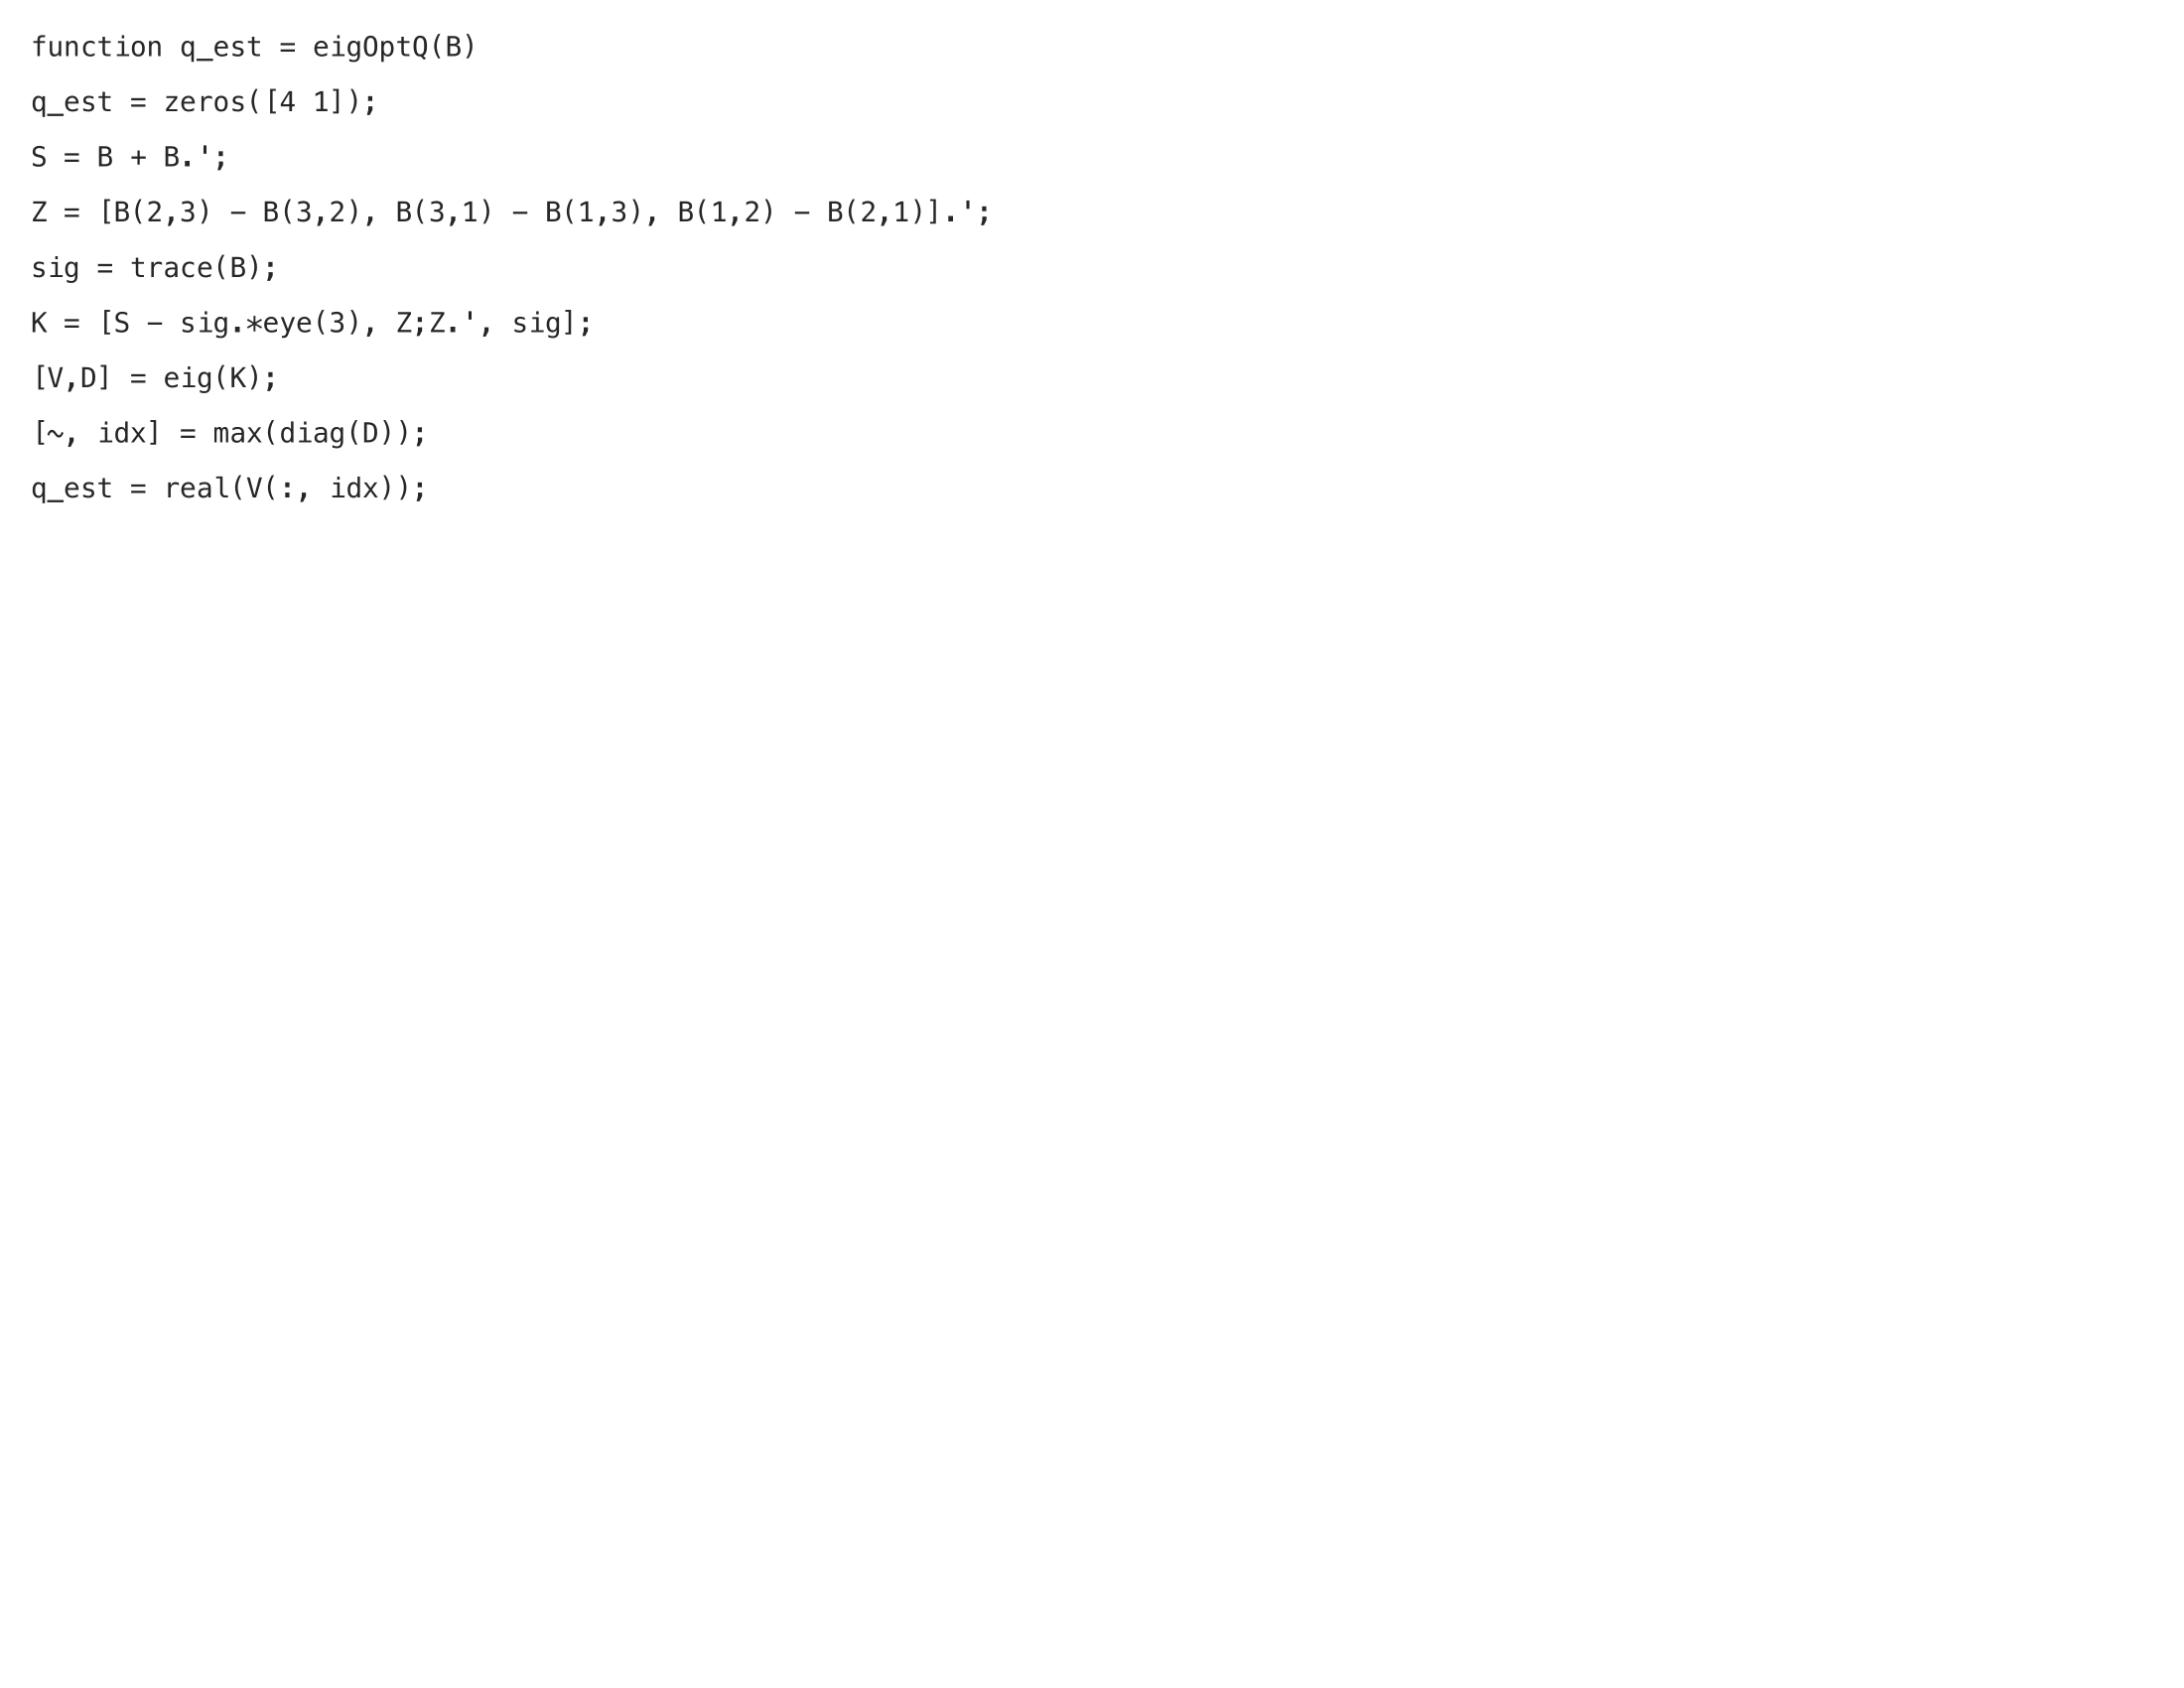
\includegraphics[trim={0cm 15cm 10cm 0cm},clip,width = 15cm]{Images/PS6/statisticalAttitude-2.png}
\end{figure}

\begin{figure}[H]
    \centering
    \captionsetup{ justification = centering }
    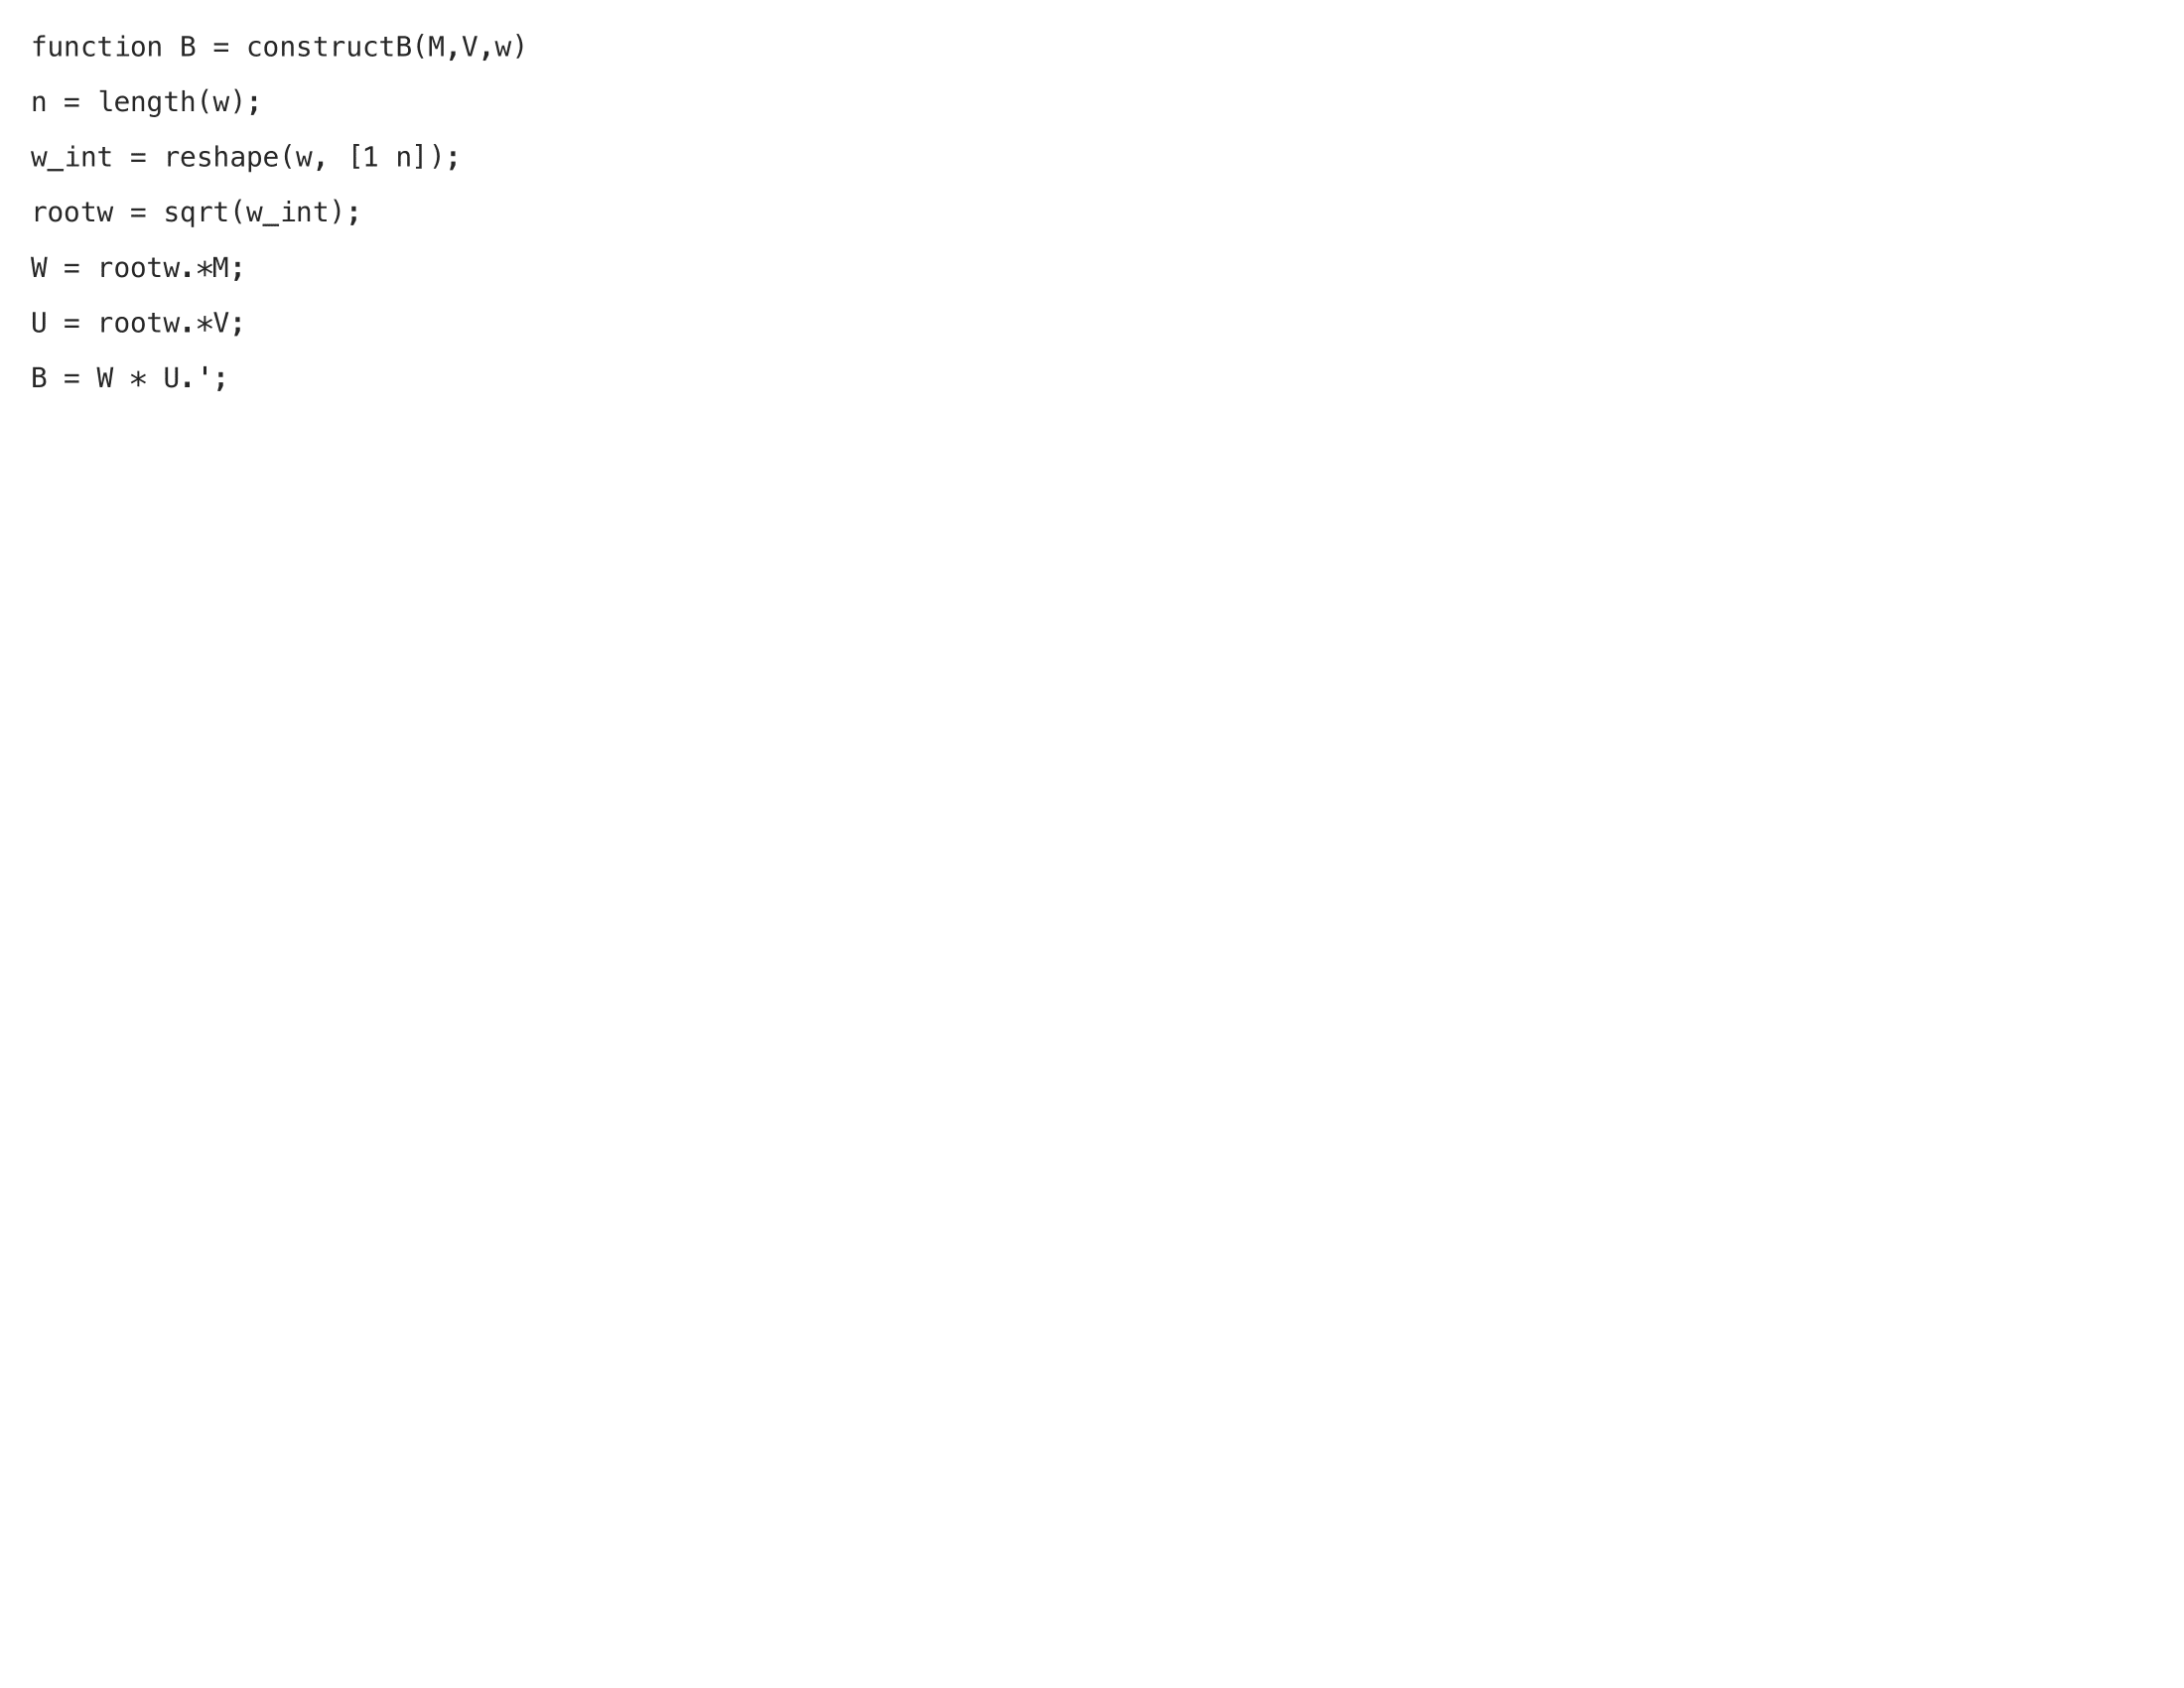
\includegraphics[trim={0cm 15cm 10cm 0cm},clip,width = 15cm]{Images/PS6/statisticalAttitude-3.png}
    \caption{Statistical Attitude Determination Model}
    \label{fig:stat_attitude}
\end{figure}

\subsubsection{Implement angular velocity measurements and the reconstruction of the attitude from those (through kinematic equations coded identically to ground truth but replicated in the spacecraft on- board computer)}

The reconstruction of the attitude from angular velocity measurements was obtained through copying the existing block to integrate the Euler equations into the on board computer (OBC). However, the angular velocity measurements were fed into the plant as opposed to a external torque. The resultant simulink diagrams are shown below.

\begin{figure}[H]
    \centering
    \captionsetup{ justification = centering }
    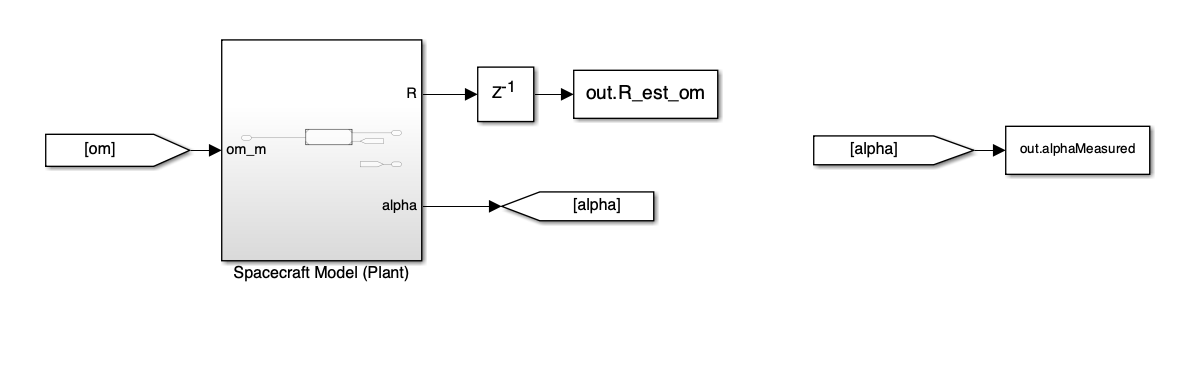
\includegraphics[width = 15cm]{Images/PS6/obc_plant_om.png}
    \caption{OBC Plant for $\omega$ Measurements}
    \label{fig:obc_plant_omega}
\end{figure}

\begin{figure}[H]
    \centering
    \captionsetup{ justification = centering }
    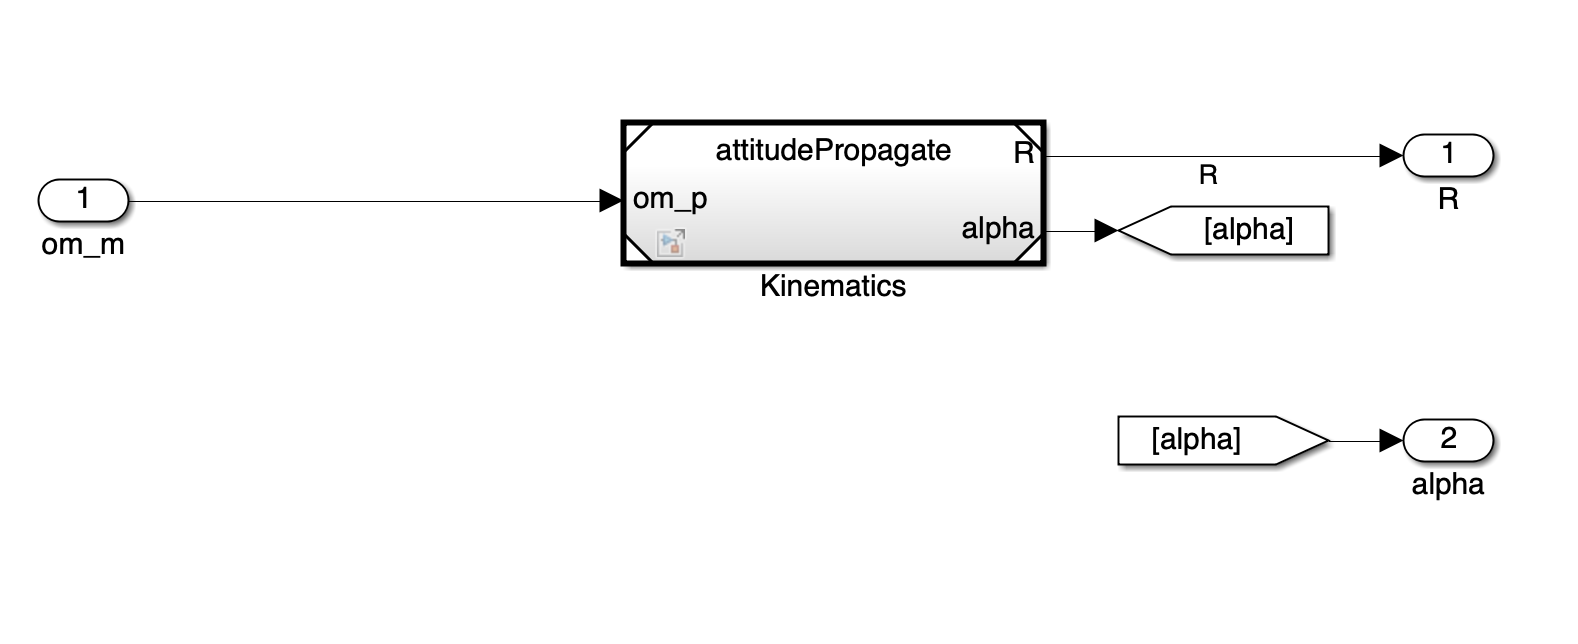
\includegraphics[width = 15cm]{Images/PS6/obc_attitudeProp_om.png}
    \caption{Attitude Propagator for $\omega$ Measurements in OBC}
    \label{fig:obc_prop_omega}
\end{figure}

The attitudePropagate block remained unchanged from previous work.

\subsection{Problem 6 - Plot the resulting estimated attitude in the absence of sensor errors. Show that it is identical to the true attitude (except for numerical errors).}

First, the deterministic attitude method was tested using the "undersampled" (2 available measurement) case. This was down with the feed through model. That is, no fictitious measurements were generated before creating a triad. The results of this simulation are seen in Figure \ref{fig:det_attitude_undersampled_default}.

\begin{figure}[H]
    \centering
    \captionsetup{ justification = centering }
    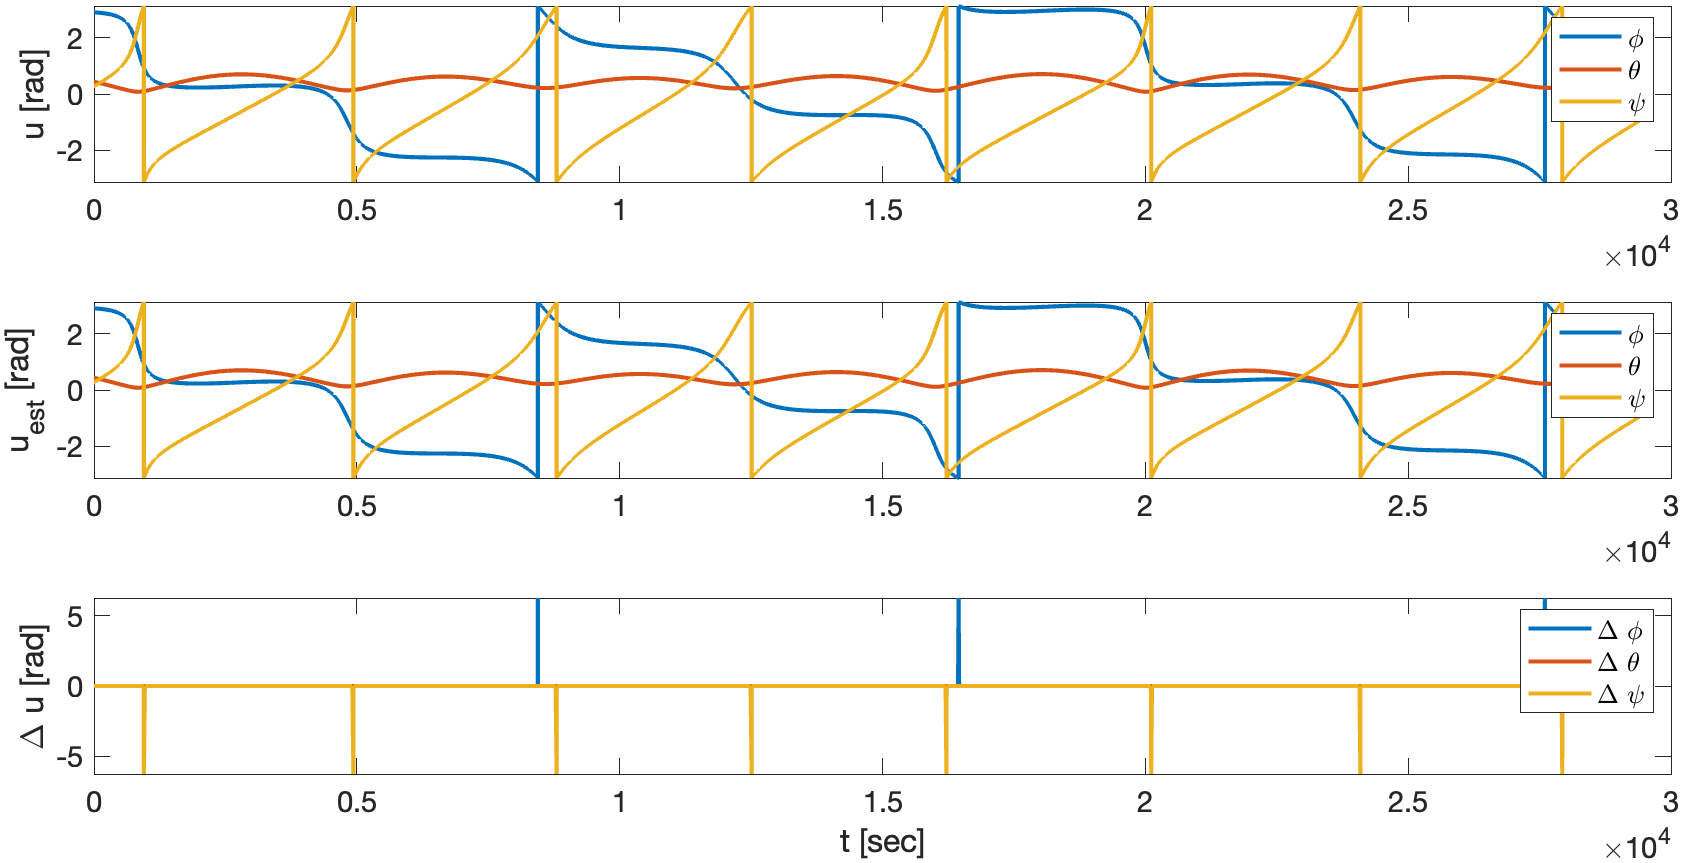
\includegraphics[width = 12cm]{Images/PS6/attitude_estimation_undersampled_det_default.png}
    \caption{Ground Truth vs. Estimated Attitude for Undersampled Deterministic Method with Feed Through Measurements}
    \label{fig:det_attitude_undersampled_default}
\end{figure}

The following test was deterministically performing attitude determination using fictitious measurements on the undersampled case. These results are seen below in Figure \ref{fig:det_attitude_undersampled_fictitious}. 

\begin{figure}[H]
    \centering
    \captionsetup{ justification = centering }
    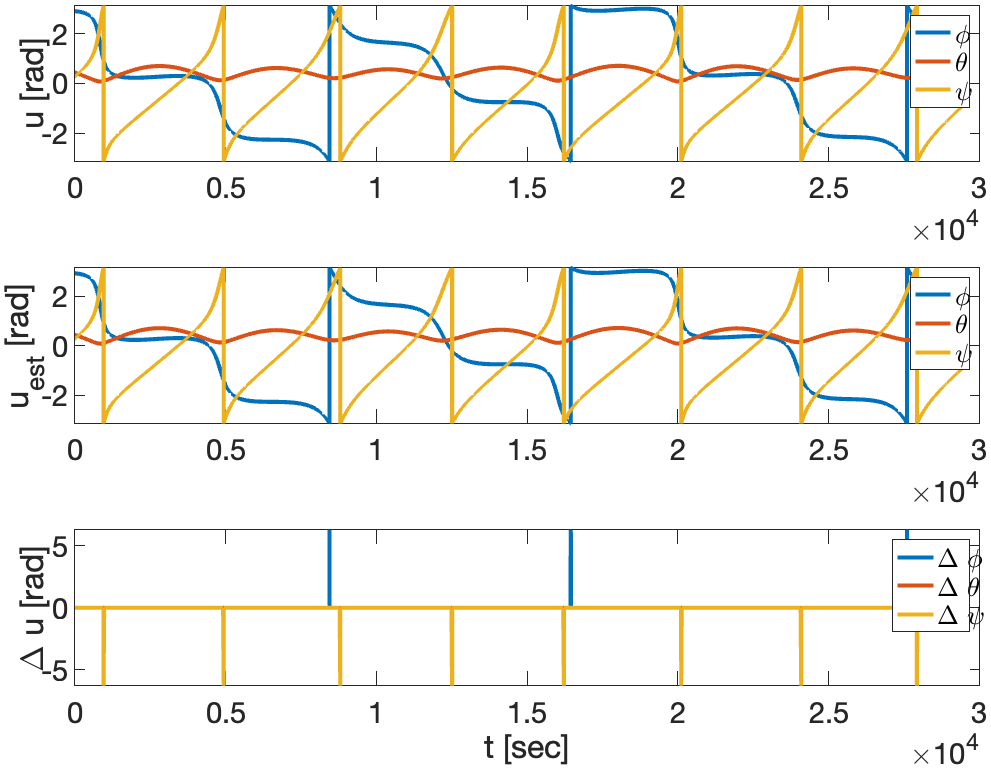
\includegraphics[width = 12cm]{Images/PS6/attitude_estimation_undersampled_det_fictitious.png}
    \caption{Ground Truth vs. Estimated Attitude for Undersampled Deterministic Method with Fictitious Measurements}
    \label{fig:det_attitude_undersampled_fictitious}
\end{figure}

The last undersampled case was on the statistical method with feed through on the measurements. These results are seen in Figure \ref{fig:stat_attitude_undersampled_default}.

\begin{figure}[H]
    \centering
    \captionsetup{ justification = centering }
    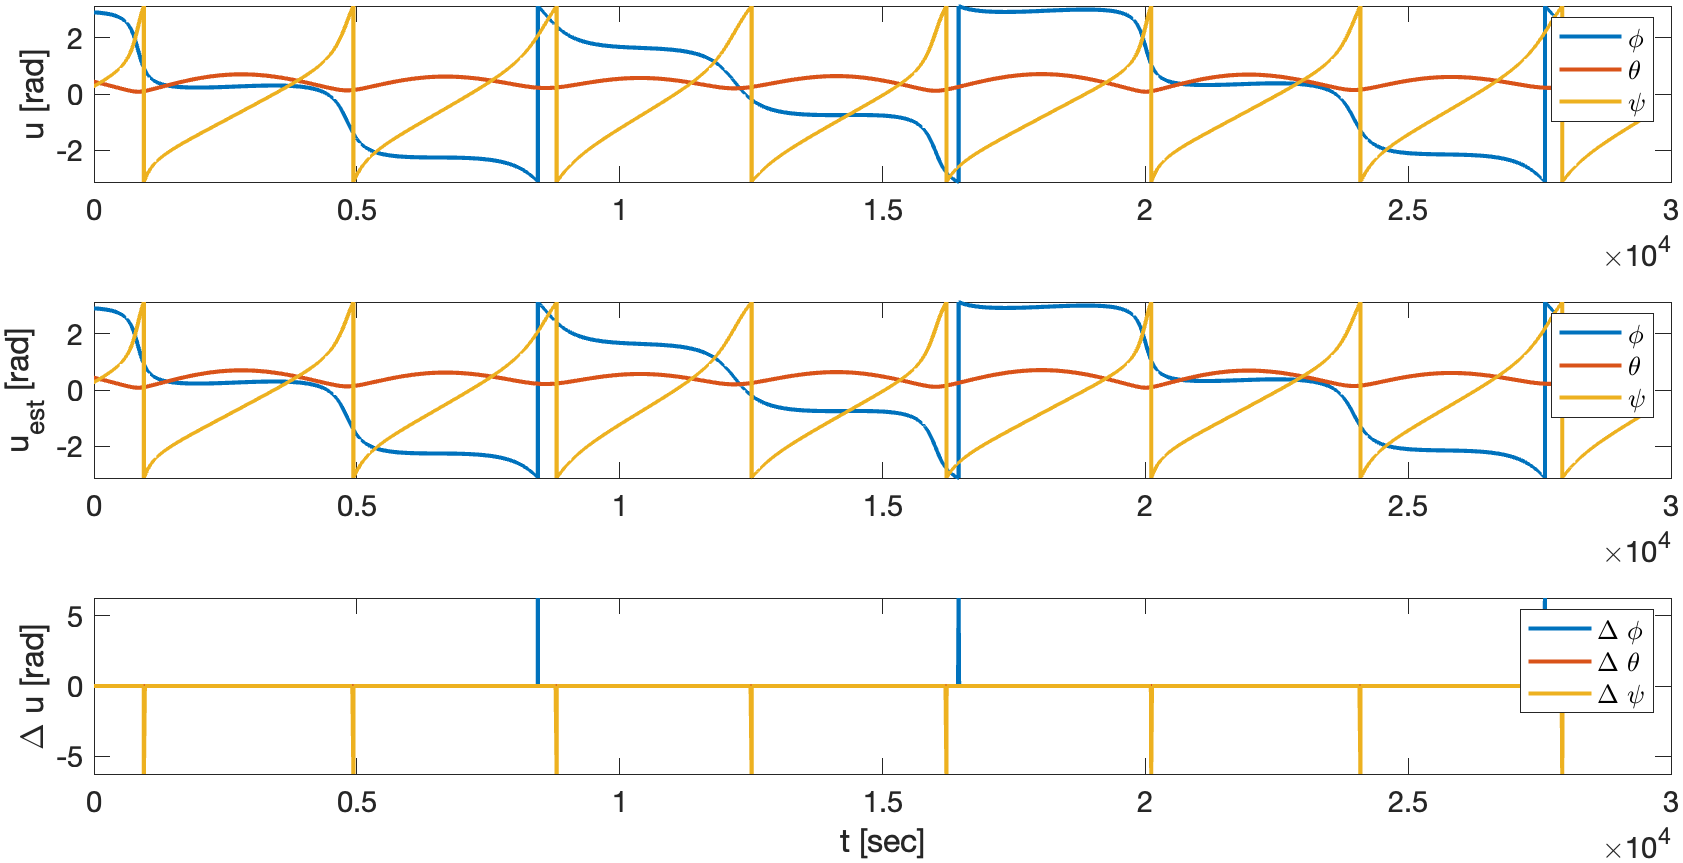
\includegraphics[width = 12cm]{Images/PS6/attitude_estimation_undersampled_q_default.png}
    \caption{Ground Truth vs. Estimated Attitude for Undersampled Statistical Method with Feed Through Measurements}
    \label{fig:stat_attitude_undersampled_default}
\end{figure}

The next step was to validate that both deterministic and statistical attitude determination methods were robust to oversampled measurements (i.e. 10 available measurements). The results of these for each respective method are shown in Figure \ref{fig:det_attitude_oversampled_default} and Figure \ref{fig:stat_attitude_oversampled_default}. 

\begin{figure}[H]
    \centering
    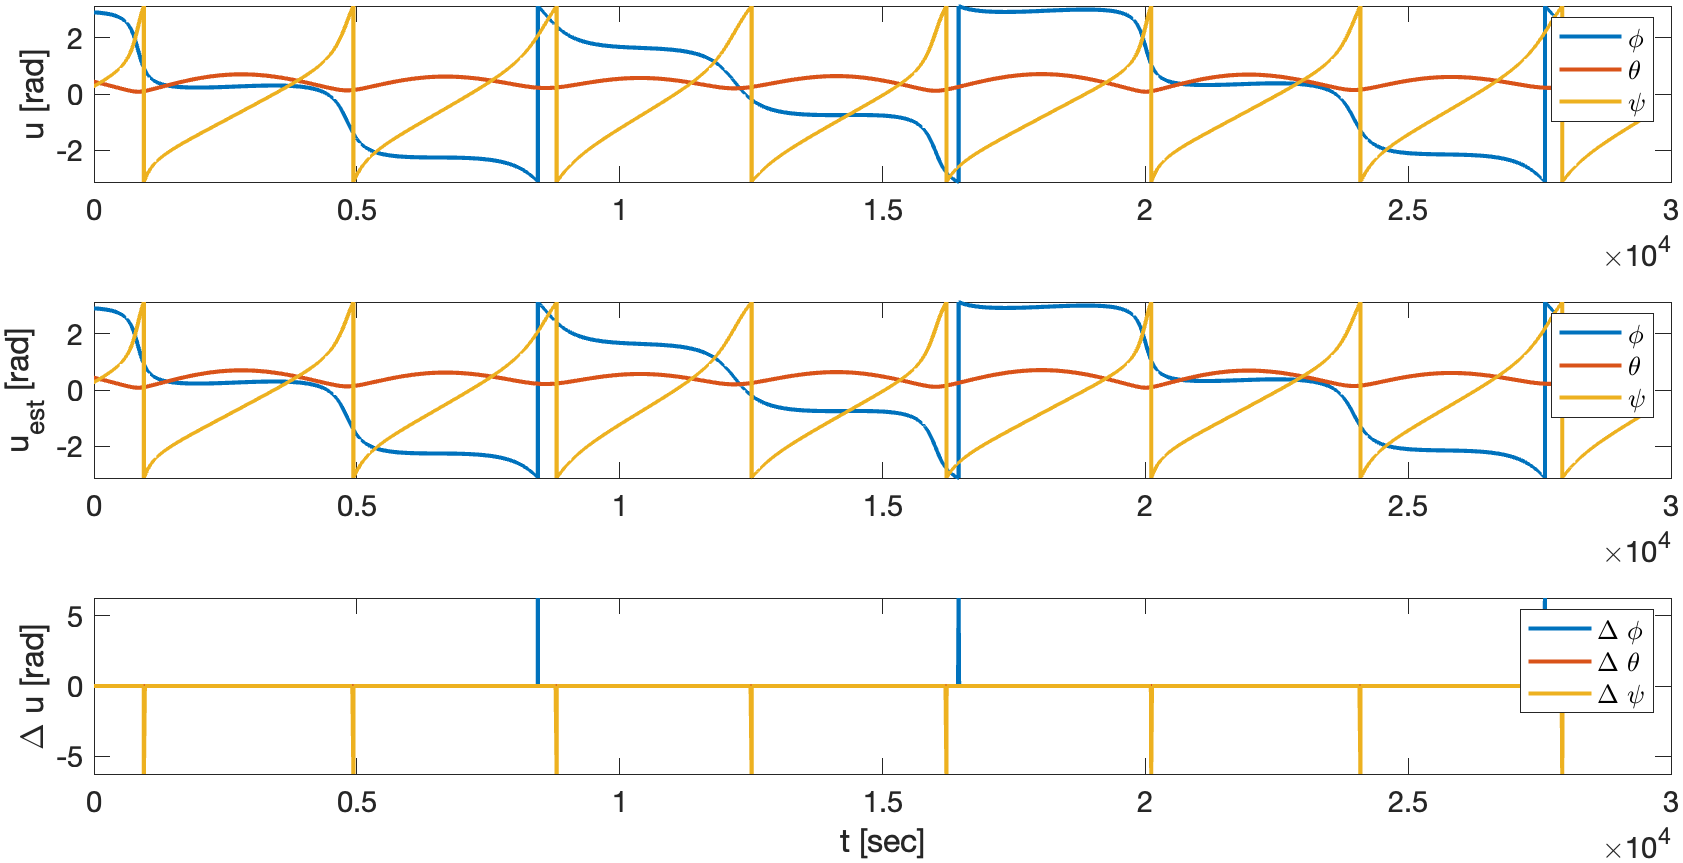
\includegraphics[width = 12cm]{Images/PS6/attitude_estimation_oversampled_det_default.png}
    \caption{Ground Truth vs. Estimated Attitude for Oversampled Deterministic Method with Feed Through Measurements}
    \label{fig:det_attitude_oversampled_default}
\end{figure}

\begin{figure}[H]
    \centering
    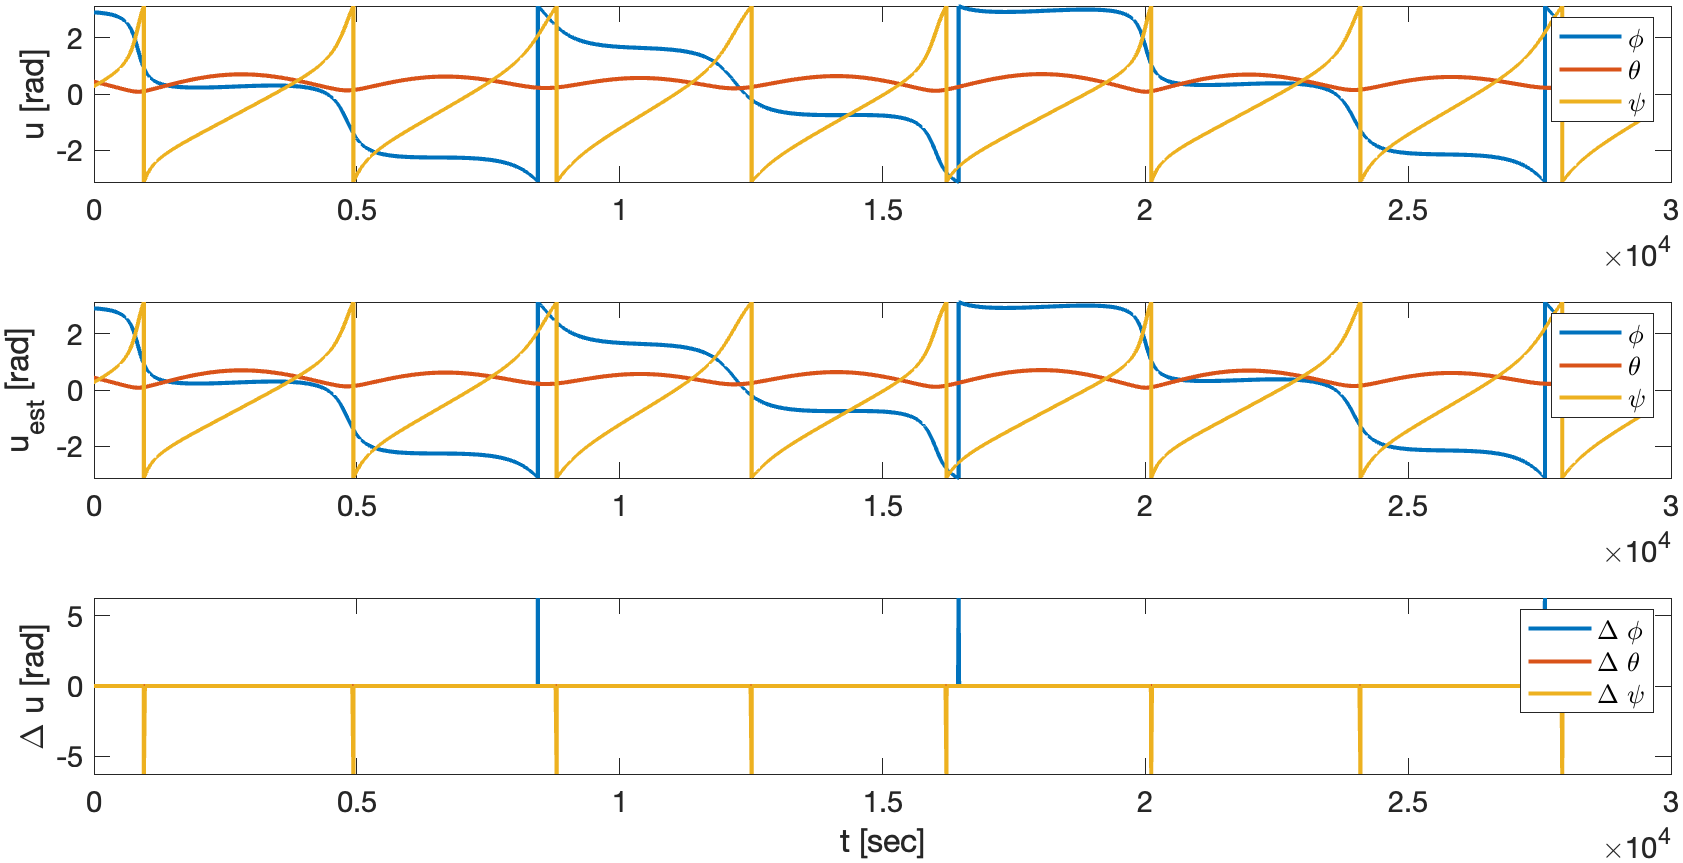
\includegraphics[width = 12cm]{Images/PS6/attitude_estimation_oversampled_q_default.png}
    \caption{Ground Truth vs. Estimated Attitude for Oversampled Statistical Method with Feed Through Measurements}
    \label{fig:stat_attitude_oversampled_default}
\end{figure}

For all cases it is seen that the error between the true state and the estimated state is nearly zero (i.e. on the order of $10^-4$). There are spikes in the error plot where singularities occur. A future fix for this might be to use quaternions or a different Euler angle sequence. 

To validate that the resultant Euler angles from the OBC $omega$ measurements were the same as the ground truth. They were co-plotted and are shown below in Figure \ref{fig:obcVsGroundOmega}.

\begin{figure}[H]
    \centering
    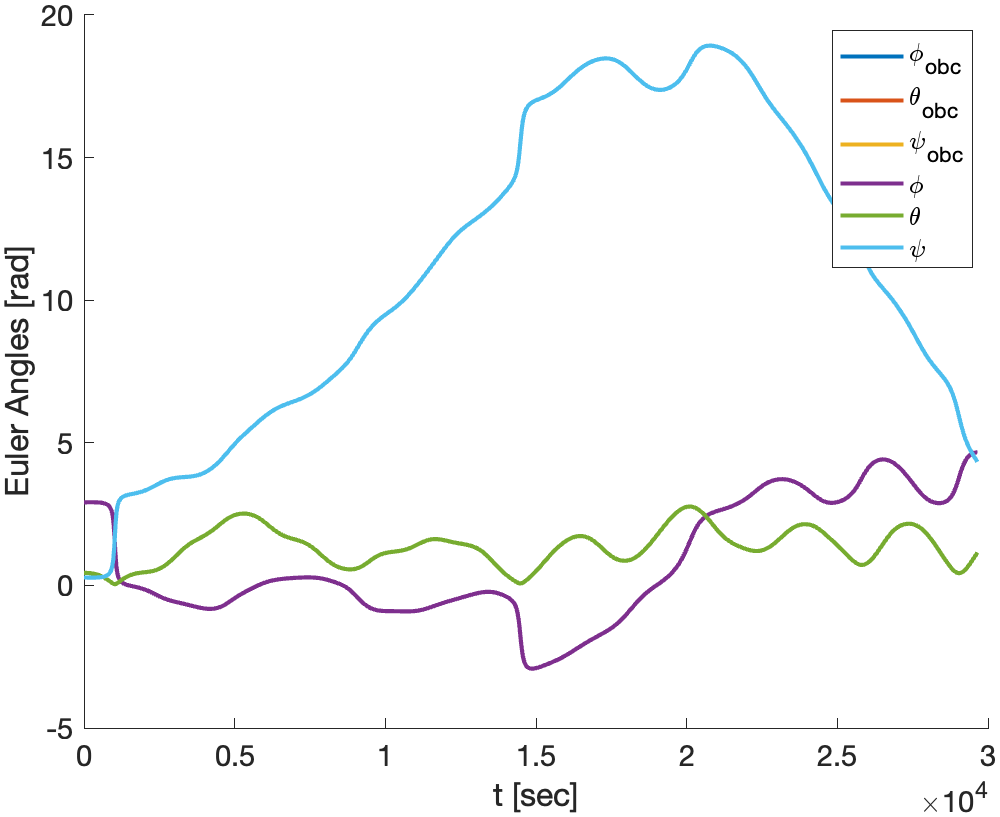
\includegraphics[width = 12cm]{Images/PS6/obcVsGroundOmegas.png}
    \caption{Ground Truth vs. Estimated Attitude for $\omega$ Measurements}
    \label{fig:obcVsGroundOmega}
\end{figure}

The plots for the ground trut perfectly overlayed those from the OBC.
\section{\Large PROBLEM SET 7}

\subsection{Problem 1 - Introduce representative (from manufacturer or Wertz or first lectures) sensor errors in the form of constant bias and Gaussian noise with given standard deviation.}

Bias and Gaussian noise were first introduced to the startracker measurements through adding them to the unit vector that represented the location of an identified star in the ECI frame. Through analyzing star trackers produced by different manufacturers, the constant bias was set to 5 arcseconds and the mean of the Gaussian noise was set to 1 arcsecond based on the values given by Honeywell for their MST satellite. From there, the position vector of the star was converted to spherical coordinates so that the the noise and bias could be added to the angular components, $\theta$ and $\phi$. The bias was directly added to the unit vector, and the noise was added through multiplying the standard deviation by a a normal distribution with mean of zero and a standard deviation of one. The resultant simulink model and code for this are show below.



\begin{figure} [H]
    \centering
    \begin{lstlisting}
function rStarUnitPerturbed = perturbMeasurements(rStarUnitSamples, rStarUnitPerturbed)

% rStarUnitPerturbed = zeros(size(rStarUnitSamples));

% Bias and standard dev from known star tracker data (Honeywell MST)
mu = 5 * (pi / 180 / 3600); % Bias error in radians (converted from 5 arcseconds)
sigma = 1 * (pi / 180 / 3600); % Standard deviation of noise in radians (converted from 1 arcseconds)

nStars = length(rStarUnitSamples(1,:));

for i = 1:nStars

    % Get one star measurement
    rStarUnit = rStarUnitSamples(:,i);

    % Convert to spherical coordinates
    x = rStarUnit(1);
    y = rStarUnit(2); 
    z = rStarUnit(3);
    r = sqrt(x^2 + y^2 + z^2);
    theta = acos(z / r);
    phi = atan2(y, x);
    
    % Calculate the displacement due to bias error
    d_bias = mu;
    
    % Generate Gaussian noise and calculate displacement
    noise = sigma .* randn(1); % Angular noise in radians
    d_noise = noise;
    
    % Add the errors to the sperical coords
    theta_perturbed = theta + d_bias + d_noise;
    phi_perturbed = phi + d_bias + d_noise;
    
    % Convert back to spherical coordinates
    x_perturbed = r * sin(theta_perturbed) * cos(phi_perturbed);
    y_perturbed = r * sin(theta_perturbed) * sin(phi_perturbed);
    z_perturbed = r * cos(theta_perturbed);
    
    u_measured = [x_perturbed; y_perturbed; z_perturbed];
    
    % Normalize the measured vector to ensure it remains a unit vector
    u_measured = u_measured ./ norm(u_measured);

    rStarUnitPerturbed(:,i) = u_measured;
    
end
end
    \end{lstlisting}
    \caption{Star Tracker Noise}
    \label{fig:starTrackerNoise}
\end{figure}

\subsection{Problem 2 - Re-apply the attitude determination algorithms from the previous pset. Plot attitude estimation error. Note that the attitude estimation error represents a rotation matrix (DCM) which quantifies how far the estimated
attitude is from the true attitude. You can use any parameterization to plot the attitude estimation errors corresponding to this DCM. Is the result consistent with the sensor bias and noise you have introduced?}


\subsection{Problem 3 - For small sensor errors, the DCM corresponds to a small rotation. Can you give an interpretation of small angles (e.g., in Euler angles and quaternions) to the obtained error DCM?}

\subsection{Problem 4 - Start modeling actual sensors in dedicated (Simulink or otherwise) subsystems which are part of the spacecraft. These models take inputs from ground-truth simulation and provides output measurements, including systematic and random errors. Take inspiration from overview of sensors discussed in class and
textbook for typical errors.}

\subsection{Problem 5 - Designing and implement the time update of a KF/EKF to obtain the best estimate of the state from the available measurements and models:}

\subsubsection{Search in literature, define, and code a state transition matrix $\Phi$ which provides your state at step k+1 based on the state at step k. Verify that the output of this propagation step is consistent with the rigorous propagation of the attitude (numerical integration). Plot propagation errors as needed.}

\subsubsection{Search in literature, define, and code a control input matrix B which provides the increment to your state at step k+1 due to a control torque at step k. Hint: optional at this stage since you do not have a controller yet.}


\subsubsection{(a) and (b) allow you to propagate the state from k to k+1 including the known control input torques. Hint: Initially you will design the filter by neglecting any control torque from your simulation.}

\subsubsection{Define and code an initial state error covariance matrix P which quantifies the uncertainty of your initial state. This can be picked as diagonal matrix with diagonal elements representing the variance of each state parameter σ2. Initially you can neglect cross-covariance terms assuming that errors of various state components are not correlated.}

\subsubsection{The time update of the EKF needs Φ, B, and P. Hint: You could increment your navigation performance by keeping the filter receptive to new measurements at steady state through the addition of constant process noise Q at each step. Initially you can define Q similar to P but much smaller (e.g., 1/10 or 1/100).}

\subsection{Problem 6 - Produce plots showing true attitude estimation errors (estimate vs truth with statistics), formal or estimated attitude estimation errors (covariance from filter). Discuss the results, do they meet expectations? How well is the true estimation error described by the formal covariance? Note that we are only implementing the time update even if we call them “attitude estimates and estimation errors”.}
\section{\Large PROBLEM SET 8}

\subsection{Problem 1 - The time update should be complete and verified at this stage. We need to include the incoming measurements. Search in literature or derive, define, and code a sensitivity matrix H which provides your state at step k+1 from your measurement vector at step k+1 (i.e., at the same current time, propagation has already been done).}

The sensitivity matrix is defined in Equation \ref{eq:general_sens_matrix} as being the Jacobian of the measurement model, $\vec{h}$, taken with respect to the state variables.

\begin{equation} \label{eq:general_sens_matrix}
    \boldsymbol{H} = \frac{\partial \vec{h}}{\partial \vec{x}}
\end{equation}

If the measurement model yields $N$ unit vectors of known direction in the inertial frame (i.e. star direction, sun direction, etc.) represented by vectors, $\vec{v}_i$, then it follows the form shown in Equation \ref{eq:attitude_meas_model}.

\begin{equation} \label{eq:attitude_meas_model}
    \vec{h}_{\alpha} = \begin{bmatrix}
        \boldsymbol{R}_{t+1 \vert t} \vec{v}_1 \\
        \boldsymbol{R}_{t+1 \vert t} \vec{v}_2 \\
        \vdots \\
        \boldsymbol{R}_{t+1 \vert t} \vec{v}_N
    \end{bmatrix} = \begin{bmatrix}
        \vec{h}_1 \\
        \vec{h}_2 \\
        \vdots \\
        \vec{h}_N
    \end{bmatrix}
\end{equation}

Therefore, the sensitivity matrix that corresponds to this measurement type is defined in Equation \ref{eq:attitude_sens_matrix}.

\begin{equation} \label{eq:attitude_sens_matrix}
    \boldsymbol{H}_{\alpha} = \begin{bmatrix}
        \boldsymbol{ \left[ h_1 \times \right] } & \boldsymbol{ \left[ h_2 \times \right] } & \dots & \boldsymbol{ \left[ h_N \times \right] }
    \end{bmatrix}^T
\end{equation}

In the state space that has been chosen for this Kalman Filter, however, there is also a component of the measurement and the component of the state that describe the angular velocity of the spacecraft about its principal axes. Tor this component of the measurement and state vector, the sensitivity matrix is simply identity, which is seen in Equations \ref{eq:vel_meas_model} and \ref{eq:vel_sens_matrix}.

\begin{equation} \label{eq:vel_meas_model}
    \vec{h}_{\omega} = \begin{bmatrix}
        \omega_x \\
        \omega_y \\
        \omega_z
    \end{bmatrix}
\end{equation}

\begin{equation} \label{eq:vel_sens_matrix}
    \boldsymbol{H}_{\omega} = \boldsymbol{I}
\end{equation}

Now constructing a block sensitivity matrix to span the full measurement model and state space, the full sensitivity matrix is shown in Equation \ref{eq:full_sens_matrix}.

\begin{equation} \label{eq:full_sens_matrix}
    \boldsymbol{H} = \begin{bmatrix}
        \boldsymbol{H}_{\alpha} & \boldsymbol{0} \\
        \boldsymbol{0} & \boldsymbol{H}_{\omega}
    \end{bmatrix} = \begin{bmatrix}
        \begin{bmatrix}
        \boldsymbol{ \left[ h_1 \times \right] } & \boldsymbol{ \left[ h_2 \times \right] } & \dots & \boldsymbol{ \left[ h_N \times \right] }
    \end{bmatrix}^T & \boldsymbol{0} \\
        \boldsymbol{0} & \boldsymbol{I}
    \end{bmatrix}
\end{equation}

The MATLAB Function within the Simulink model that is used to compute this is seen in Figure \ref{fig:sens_matrix_function}.

\begin{figure} [H]
    \centering
    \captionsetup{ justification = centering }
    \begin{lstlisting}
function H = constructH(h)

h_att = h(1:end-3);
% h_om = h(end-2:end);

n = uint32(length(h_att));

H_att = zeros([3, n]);

iters = n/3;

for i=1:iters
    H_att(:, (3*(i-1) + 1):(3*(i-1) + 1 + 2)) = vcross( h( (3*(i-1) + 1):(3*(i-1) + 1 + 2) ) ).';
end

H = [H_att.', zeros(size(H_att.'));
    zeros([3 3]), eye(3)];

    function V = vcross(v)
        V = [0, -v(3), v(2);
            v(3), 0, -v(1);
            -v(2), v(1), 0];
    end

end
    \end{lstlisting}
    \caption{Sensitivity Matrix Function}
    \label{fig:sens_matrix_function}
\end{figure}

\subsection{Problem 2 - Define and code your constant measurement error covariance matrix R which quantifies the uncertainty of your measurements. This can be picked as diagonal matrix with diagonal elements representing the variance of each parameter $\sigma^2_m$. Hint: If your instrument is well characterized you can use $\sigma_m$ applied in your simulation to generate the measurements from your ground-truth.}

For the error covariance matrix R, the manufacturer data for the standard deviation of the noise for each of the sensors was used. As stated in the previous homework, the standard deviations for each of the sensors are as follows.

\begin{align*}
    \sigma_{StarTracker} &= 0.000277778 \degree\\
    \sigma_{Magnetometer} &= 0.0011459 \degree\\
    \sigma_{Gyro} &= 0.014 \degree / s\\
\end{align*}

The standard deviation for the noise introduced by each of the sensors was converted to be in radians as opposed to degrees and squared before going into $\boldsymbol{R}$.

\begin{equation*}
    \boldsymbol{R} = \begin{bmatrix} 
        4e-10 & 0 & 0 & 0 & \dots & 0 & 0 & 0 & 0\\
        0 & 4e-10 & 0 & 0 &  & \vdots & \vdots & \vdots & \vdots \\
        0 & 0 & 4e-10 & 0 &  & \vdots & \vdots & \vdots & \vdots \\
        0 & 0 & 0 & 2.35e-11 &  & \vdots & \vdots & \vdots & \vdots \\
        \vdots & \vdots & \vdots & &  \ddots &\vdots &\vdots&\vdots & \vdots\\
        0 & 0 & 0 & 0 &  & 2.35e-11 & 0 & 0 & 0 \\
        \vdots & \vdots & \vdots & \vdots & & 0 & 5.97e-8 & 0 & 0 \\
        \vdots & \vdots & \vdots & \vdots & & 0 & 0 & 5.97e-8 & 0  \\
        \vdots & \vdots & \vdots & \vdots &  & 0 & 0 & 0 & 5.97e-8\\
    \end{bmatrix} 
\end{equation*}
\begin{equation*}
    \boldsymbol{R} 
    = 2 \boldsymbol{I}
\end{equation*}

\subsection{Problem 3 - Compute your modelled measurement vector at step k+1 from your state at step k+1. This transformation can be rigorous (non-linear, EKF) or approximate (linear, KF).}

The full concatenated measurement model is computed using both Equations \ref{eq:attitude_meas_model} and \ref{eq:vel_meas_model}. This full measurement model, seen in Equation \ref{eq:full_meas_model}, at this stage in simulation is supposed be be used at every time step. The model that computes this measurement model is seen in Figure \ref{fig:simulink_meas_model}.

\begin{equation} \label{eq:full_meas_model}
    \vec{h} = \begin{bmatrix}
        \vec{h}_{\alpha} \\ \vec{h}_{\omega}
    \end{bmatrix} = \begin{bmatrix}
        \boldsymbol{R}_{t+1 \vert t} \vec{v}_1 \\
        \boldsymbol{R}_{t+1 \vert t} \vec{v}_2 \\
        \vdots \\
        \boldsymbol{R}_{t+1 \vert t} \vec{v}_N \\
        \omega_x \\
        \omega_y \\
        \omega_z
    \end{bmatrix}
\end{equation}

\begin{figure}[H]
    \centering
    \captionsetup{ justification = centering }
    \includegraphics[width = 12cm]{}
    \caption{Simulink Model for Measurement Model Computation}
    \label{fig:simulink_meas_model}
\end{figure}

The assumption that this full model will be used at is not necessarily true for real space systems. This is due to varying availability of measurements from different sensors. Thus, a typical Kalman Filter on-board a spacecraft will handle measurements sequentially as they are made available. This functionality may be explored further in future work.

\subsection{Problem 4 - Compute your pre-fit residuals z by differencing modelled and actual measurement vector at k+1.}

The residual $\vec{z}$ is computed using Equation \ref{eq:meas_residual}.

\begin{equation} \label{eq:meas_residual}
    \vec{z} = \vec{y} - \vec{h}
\end{equation}

\subsection{Problem 5 - The measurement update of the EKF needs H, P, R, and z to compute the Kalman gain K, the new estimated state and its associated covariance matrix.}

The Kalman gain is computed using Equation \ref{eq:kalman_gain}.

\begin{equation} \label{eq:kalman_gain}
    \boldsymbol{K}_t = \boldsymbol{\Sigma}_{t+1 \vert t} \boldsymbol{H}_t^T \left( \boldsymbol{H} \boldsymbol{\Sigma}_{t \vert t-1} \boldsymbol{H}_t^T + \boldsymbol{R}_t \right)^{-1}
\end{equation}

The measurement update for the state mean and covariance are computed using Equations \ref{eq:state_mean_update} and \ref{eq:state_covariance_update}.

\begin{equation} \label{eq:state_mean_update}
    \vec{x}_{t+1 \vert t+1} = \vec{x}_{t+1 \vert t} + \boldsymbol{K}_t \vec{z}_t
\end{equation}

\begin{equation} \label{eq:state_covariance_update}
    \boldsymbol{\Sigma}_{t+1 \vert t+1} = \boldsymbol{\Sigma}_{t+1 \vert t} - \boldsymbol{K}_t \boldsymbol{H}_t \boldsymbol{\Sigma}_{t+1 \vert t}
\end{equation}

The following MATLAB function, shown in Figure \ref{fig:meas_update_matlab_func}, uses the current sensitivity matrix, state covariance, measurement noise covariance, and the residual to compute an updated state mean and covariance estimate.

\begin{figure}
    \centering
    \captionsetup{ justification = centering}
    \begin{lstlisting}
function [mu_plus, Sig_plus] = measUpdate(mu_minus, Sig_minus, z, H, R_noise)

K = (Sig_minus * H.')/(H * Sig_minus * H.' + R_noise);

mu_plus = mu_minus + K * z;
Sig_plus = Sig_minus - K * H * Sig_minus;
    \end{lstlisting}
    \caption{Measurement Update Function}
    \label{fig:meas_update_matlab_func}
\end{figure}

\subsection{Problem 6 - Compute your post-fit residuals z by differencing modelled and actual measurement vector at k+1 using your new state. These should be smaller than the pre-fit residuals and should capture the standard deviation of your measurements at steady state.}

Following the measurement update, for a MEKF, the reset step must take place before the post fit residuals are computed. This update step follows Equation \ref{eq:quat_reset_step}.

\begin{equation} \label{eq:quat_reset_step}
    \vec{q}_{t+1 \vert t+1} = \begin{bmatrix}
        1 & -\alpha_1/2 & -\alpha_2/2 & -\alpha_3/2 \\
        \alpha_1/2 & 1 & \alpha_3/2 & -\alpha_2/2 \\
        \alpha_2/2 & -\alpha_3/2 & 1 & \alpha_1/2 \\
        \alpha_3/2 & \alpha_2/2 & -\alpha_1/2 & 1
    \end{bmatrix} \vec{q}_{t+1 \vert t}
\end{equation}

The model that computes this update step is shown in Figure \ref{fig:quat_reset_step}.

\begin{figure}[H]
    \centering
    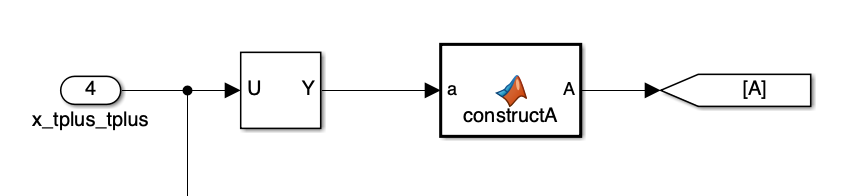
\includegraphics[width = 10cm]{Images/PS8/quat_update_2.png}
    \includegraphics[width = 8cm]{Images/PS8/quat_update_1.png}
\end{figure}

\begin{figure}[H]
    \centering
    \captionsetup{ justification = centering }
    \begin{lstlisting}
function A = constructA(a)

ax = a(1);
ay = a(2);
az = a(3);

A = eye(4) + (1/2).*[0, -ax, -ay, -az;
                    ax, 0, az, -ay;
                    ay, -az, 0, ax;
                    az, ay, -ax, 0];
    \end{lstlisting}
    \caption{Simulink Model for Reset Step}
    \label{fig:quat_reset_step}
\end{figure}

Once this is computed, a rotation matrix can be obtained from the post-reset quaternion and used to recompute the measurement model. Now the residual can be computed using again Equation \ref{eq:meas_residual}.

For any plots and analysis regarding these residuals, the norm of this residual vector will be taken.

\subsection{Problem 7 - Produce plots showing true attitude estimation errors (estimate vs truth with statistics at steady state), formal or estimated attitude estimation errors (covariance from filter), pre- and post-fit residuals (with statistics at steady state), etc. Discuss the results, do they meet expectations? Is the true estimation error well described by the formal covariance? Are the measurements residuals consistent with the applied measurement errors? Hint: show estimation errors, do not overlap state estimate with reference truth.}

\subsection{Problem 8 - Start thinking/planning possible upgrades for the final project deliverable. Upgrades can go in several directions tailored to your project needs. For example, define different modes for attitude estimation using different sensors and algorithms based on your concept of operations. What would it take to implement a UKF instead of an EKF? Can you improve your dynamics and measurement models? Can you use measurements that are more representative of what your sensors are going to actually provide you?}

In the previous homework, the sensors were only modelled to the depth of assuming that they output unit vector measurement of the star location or gravitational field. 
\section{\Large PROBLEM SET 9}

\subsection{Problem 1 - Start selecting and sizing your actuators using the basic dimensional formulas provided in class (Wertz, SMAD) based on your perturbation environment and attitude slew objectives. Provide rationale for choice.}

As shown in Section \ref{sec:pertTorques}, the total torque from aerodynamic drag, solar radiation, gravity, and magnetic disturbances are shown in Figure \ref{fig:all_torque} and again below in Figure \ref{fig:all_torque_hw9} for completeness.

\begin{figure}[H]
    \centering
    \captionsetup{ justification = centering }
    \includegraphics[width = 12cm]{Images/PS6/all_torque.png}
    \caption{Total Torque}
    \label{fig:all_torque_hw9}
\end{figure}

In this plot it can be seen that the maximum torque is about 0.035 Nm. Due to the criticality of the actuators to the mission, a safety factor of 2.5 was selected to ensure that the selected actuators would be well equipped to handle perturbations well outside of the expected range. Multiplying the safety factor by the maximum perturbation torque resulted in a required maximum torque of 0.0875 Nm. Due to the nature of the mission, it isn't required for the satellite to complete fast slew maneuvers to switch between different modes of operation. Because the satellite is in a sun-synchronous orbit, and the sensors will always be earth pointing, there isn't a need to quickly slew between the science mode of operation where the data collection is prioritized to the charging mode of operation where the solar arrays must be pointed towards the sun. Because of this, it is sufficient to size the actuators to handle the manuevers that are needed to correct for perturbations torques and not for fast slew maneuvers.

In order to ensure that the chosen actuators were able to produce the required maximum torque, available data sheets for momentum/reaction wheels and magnetorquers were analyzed. For reaction wheels, the Rocket Lab 12.0 Nms RW4 [Rad-Hard] and RW5 [Standard] were analyzed as well as the Bradford Aerospace High Torque Reaction Wheel for Satellites. Their maximum angular momentum and torque outputs are tabulated in Table \ref{table:rw}.

\begin{table}
\begin{tabular}{c|c|c}
    & Maximum Angular Momentum (Nms) & Maximum Torque (Nm) \\
    \hline 
    Bradford & 45 & 0.265 \\
    \hline 
    Rocket Lab & 12 & 0.2 \\
\end{tabular}
\caption{Reaction Wheel Data}
\label{table:rw}
\end{table}

It can also be noted that for the Bradford reaction wheel the torque rise/fall time was listed as 80 ms. Because of this short rise time, the initial angular momentum of the reaction wheel can be approximated as being anything between zero and the maximum value. For the magnetorquer, the maximum and nominal dipole moments were collected for the AAC Clyde Space MTQ800 magnetorquer and are tabulated in Table \ref{table:magnetorquer}.

\begin{table}
\begin{tabular}{c|c|c}
    & Maximum Dipole Moment (Am$^2$) & Nominal Dipole Moment (Am$^2$) \\
    \hline 
    AAC & 30 & 15 \\
\end{tabular}
\caption{Magnetorquer Data}
\label{table:magnetorquer}
\end{table}

While the exact torque output wasn't given in the specifications for the magnetorquer, it can be assumed that it is between 5e-4 and 5e-1 Nm for the given specifications. 

Due to the reaction wheels being large enough to handle the perturbation torques and the magnetorquers being better suited for fine tuning, we decided to use a combination of a set of reaction wheels and magnetorquers for the satellite.

\subsection{Problem 2 - Start modeling actuators in dedicated (Simulink) subsystems which are part of the spacecraft. These models take inputs from ground-truth simulation and provides output control torques to be directly fed into the Euler equations, including systematic and random errors. Plot output vs input of actuator model. Hint: for the rest of this problem set you should remove all sensing and actuation errors for verification purposes.}

For our actuators, we modelled a reaction wheel, momentum wheel, and a magnetorquer. For the reaction wheel and momentum wheel, we started with the Euler equation shown below.

\begin{equation}
    \Vec{\dot L}_t + \Vec{\omega} \times \Vec{L}_t = \Vec{M}
\end{equation}

Substituting in $\Vec{L}_t = \Vec{I} \Vec{\omega} + \Vec{A} \Vec{L}_w$ where $\Vec{A}$ is used to bring the angular momentum of the wheels into the principle axes into the above equation gives the full Euler equation.

\begin{equation}
    \Vec{I} \Vec{\dot \omega} + \Vec{\dot I} \Vec{\omega} + \Vec{A} \Vec{\dot L}_w + \Vec{\dot A} \Vec{L}_w + \Vec{\omega} \times \Vec{I} \Vec{\omega} + \Vec{\omega} \times \Vec{A} \Vec{L}_w = \Vec{M}
\end{equation}

For one reaction wheel and one momentum wheel, the equation can be simplified to the form shown below.

\begin{equation}
    \Vec{\dot L}_w = \Vec{A}^* \left( - \Vec{M}_c - \Vec{\omega} \times \Vec{A} \Vec{L}_w \right)
\end{equation}

From substituting in moment of inertias and angular velocities and linearizing, we obtain the following set of equations.

\begin{align}
    I_x (\Ddot{\alpha}_x - n \dot \alpha_y ) + (I_z - I_y) ( n \dot \alpha_y + n^2 \alpha_x ) + I_{wz}\Bar{\omega}_{wz} ( \dot \alpha_y + n \alpha_x) - I_{wy} \omega_{wy} n = 0
\end{align}

\begin{align*}
    I_x (\Ddot{\alpha}_y - n \dot \alpha_x ) + (I_z - I_y) ( n \dot \alpha_x - n^2 \alpha_y ) - I_{wz}&\Bar{\omega}_{wz} ( \dot \alpha_x + n \alpha_y) + I_{wy} \omega_{wy} - 3 n^2 (I_x - I_z) \alpha_y = 0 \\
    I_z \Ddot{\alpha}_z + I_{wz} \dot \omega_{wz} +& 3n^2\left( I_y - I_x \right) \alpha_z = 0 \\
    I_{wy} \dot \omega_{wy} = M_{cy} ;& I_{wz} \dot \omega_{wz} = M_{cz}
\end{align*}


The simulink model that was used to implement this is shown below in Figures \ref{fig:simulink_mw} and \ref{fig:rwCode}.

\begin{figure}[H]
    \centering
    \captionsetup{ justification = centering }
    \includegraphics[width = 15cm]{Images/PS9/momentumWheelModel.png}
    \caption{Simulink Model for Momentum Wheel}
    \label{fig:simulink_mw}
\end{figure}

\begin{figure}[H]
    \centering
    \captionsetup{ justification = centering}
    \begin{lstlisting}
function Lwdot = Mc2Lwdot(Mc, omega, A, Lw)

Lwdot = pinv(A) * (- Mc - cross(omega, A * Lw));
    \end{lstlisting}
    \caption{Reaction Wheel Function}
    \label{fig:rwCode}
\end{figure}

For the magnetorquer, the following Euler equation was used to get output torque where $A$ = [0 0 1]$^T$.

\begin{equation}
    \Vec{M}_c = \Vec{m} \times \Vec{B} + \Vec{A} \Vec{\dot L}_w
\end{equation}

The same simulink model used to obtain the magnetic field for both the magnetic disturbances and magnetometer was used, and the new overall simulink model is shown below.

\begin{figure}[H]
    \centering
    \captionsetup{ justification = centering }
    \includegraphics[width = 15cm]{Images/PS9/magnetorquerModel.png}
    \caption{Simulink Model for Magnetorquer}
    \label{fig:simulink_magnetorquer}
\end{figure}

\begin{figure}[H]
    \centering
    \captionsetup{ justification = centering}
    \begin{lstlisting}
function Mout = fcn(m, Ldot, B)

Mout = cross(m,B) + [0;0;1] * Ldot;
    \end{lstlisting}
    \caption{Magnetorquer Function}
    \label{fig:mtCode}
\end{figure}

The input and output of both of these actuators are shown below in Figures \ref{} and \ref{}.

\begin{figure}[H]
    \centering
    \captionsetup{ justification = centering }
    \includegraphics[width = 15cm]{Images/PS9/reaction_wheel_model_output.png}
    \caption{Output for Reaction Wheel}
    \label{fig:rwOutput}
\end{figure}

\begin{figure}[H]
    \centering
    \captionsetup{ justification = centering }
    \includegraphics[width = 15cm]{Images/PS9/simple_magnetorquer_plus_wheel_model_output.png}
    \caption{Output for Reaction Wheel and Magnetorquer}
    \label{fig:mtOutput}
\end{figure}

\subsection{Problem 3 - Start designing and implementing a linear control law which provides the desired behavior of the dynamic system (damping and frequency) by a feedback done on the control tracking errors. Try using both a small angle approximation and a non-linear approach in defining the control tracking errors used in the control law. Hint: this task requires that you linearize the Euler equations and that you show how the gains of the linear control law are derived, also start applying the control law by assuming that the actuators are doing their job ideally (no actuation equations, no saturation or other limits). Selection of gains can be done through standard PD, pole placement or LQR approaches.}

A PD controller was used for this task. The nonlinear approach was done by taking the error produced from the sensor measurements, $R$, and producing the inverse skew matrix through the function shown in Figure \ref{fig:smallThetaCode}.

\begin{figure}[H]
    \centering
    \captionsetup{ justification = centering}
    \begin{lstlisting}
function alpha = inv_skw(R)

alpha = zeros([3 1]);

alpha(1) = (R(2,3) + (-R(3,2)))/2;
alpha(2) = (R(3,1) + (-R(3,1)))/2;
alpha(3) = (R(1,2) + (-R(2,1)))/2;
    \end{lstlisting}
    \caption{Small Angle Approximation Function}
    \label{fig:smallThetaCode}
\end{figure}

The small angle approximation was also attempted, but since the nonlinear approximation was functioning and the two approaches behaved the same in the relevant regime, it wasn't explored further. From here, $\alpha$ and the angular velocity errors from the gyroscope were fed into the following equation for the PD control law as $e_\theta$ and $e_\omega$.

\begin{equation}
    \Vec{I} \Vec{\dot \omega} = \Vec{\tau} - \Vec{\omega} \times (\Vec{I} \Vec{\omega})
\end{equation}

\begin{equation}
    - \dot \omega_{desired} = -K_p e_\theta - K_d e_\omega
\end{equation}

The simulink implementation of this is shown below.

\begin{figure}[H]
    \centering
    \captionsetup{ justification = centering }
    \includegraphics[width = 15cm]{Images/PS9/controllerModel.png}
    \caption{Simulink Model for Controller}
    \label{fig:controllerSimulink}
\end{figure}

\begin{figure}[H]
    \centering
    \captionsetup{ justification = centering }
    \includegraphics[width = 15cm]{Images/PS9/PDController.png}
    \caption{Simulink Model for PD Gains}
    \label{fig:PDsimulink}
\end{figure}

The design the $k_p$ and $k_d$ gains, the euler equations were linearized to follow the form shown below.

\begin{equation}
    I \Vec{\Ddot{\alpha}} + k_d  \Vec{\dot \alpha} + k_p \alpha = 0
\end{equation}

Additionally, the desired characteristic equation for the closed-loop transfer function is $s^2 + 2\zeta\omega_n s +\omega_n^2$ where $\zeta$ is the damping ratio and $\omega_n$ is the natural frequency. Because of this, $K_p = \omega_n^2 I_{axis}$ and $K_d = 2\zeta\omega_n I_{axis}$. From this, a damping ratio of $\sqrt{2}/2$ and a frequency of 50n were chosen to obtain $k_p$ and $k_d$.

It is also important to note that since there are currently bugs in our Kalman filter, the controller is currently getting fed ground truth to aboid residual errors.


\subsection{Problem 4 - Start plotting all the relevant quantities of your simulation, including attitude determination errors, attitude control errors, control actions (along all axes), etc. Hint: stress difference between what the ADCS believes, and what the spacecraft is actually doing. This affects estimation, control errors, and control actions.}

Due to bugs in our Kalman filter, the current attitutude determination error is getting plotted using the q-method as opposed to the MEKF.

%%%%%%%%%%%%%%%%%%%%%%%%%%%%%%%%%%%%%%%%%%%%%%%%%%%%%%%%%%%%%%%%%%%%%%%%%%%%%%%%%%%%%%%%%%%%%%%%%%%%%%%%%%%%%%%%%%%%%%%%%%%%%%%%%%%%%%%%%%%%%%%%%%%%%%%%%%%%%%%%%%%%%%%%%%%%%%%%%%%%%%%%%%%%%%%%%%%%%%%%%%%%%%%%%%%%%%%%%%% 
\section{\Large CONCLUSION}

\bibliographystyle{IEEEtran}
\bibliography{refs}


\end{document}